%! Author = Omar Iskandarani
%! Title = Swirl Clock Appendices
%! Date = May 23, 2025
%! Affiliation = Independent Researcher, Groningen, The Netherlands
%! License = CC-BY 4.0
%! ORCID = 0009-0006-1686-3961
%! DOI = 10.5281/zenodo.15707931

\documentclass[a4paper,12pt]{article}
\usepackage{../vamstyle}
\usepackage{tikz}
\usepackage{amsmath}
\usepackage{amssymb}
\usepackage{hyperref}
\usetikzlibrary{arrows.meta, positioning, shapes.multipart}
\usepackage{amsthm}
\newtheorem{theorem}{Theorem}[section]
\newtheorem{lemma}[theorem]{Lemma}
\usepackage{booktabs}
\usepackage{array}
\usepackage{bm}

\title{Swirl Clock Appendices\\[0.5em]}
\author{
    Omar Iskandarani\thanks{
        Independent Researcher, Groningen, The Netherlands.\\
        Email: \texttt{info@omariskandarani.com}\\
        ORCID: \href{https://orcid.org/0009-0006-1686-3961}{0009-0006-1686-3961}\\
        DOI: \href{https://doi.org/10.5281/zenodo.15707931}{10.5281/zenodo.15707931}
    }
}
\date{\today}


\begin{document}
    \maketitle
    \vspace{-2ex}


\begin{abstract}
This appendix supplements the main Swirl Clocks paper within the Vortex \AE{}ther Model (VAM) framework by presenting detailed derivations, interpretations, and physical consequences of vortex-induced temporal dynamics. It formally defines and interrelates the layered time constructs—Aithēr-Time \( \mathcal{N} \), Chronos-Time \( \tau \), Swirl Clock phase \( S(t) \), Vortex Proper Time \( T_v \), and the Kairos transition moment \( \kappa \)—as distinct but interacting manifestations of causal flow in a structured æther. Building on the premise that time dilation emerges not from spacetime curvature but from local swirl energy and circulation, we derive dilation formulas from first principles in vortex hydrodynamics, Bernoulli pressure gradients, and tangential \ae{}ther velocities. The clock slowdown is shown to follow an exponential decay with radial distance from the vortex core, recovering gravitational time delay analogs without invoking general relativity.

Multiple derivation paths—energetic, topological, and angular momentum based—are explored and numerically validated. We further examine temporal phase accumulation \( S(t) \), its role in quantum coherence, and its significance in low-energy nuclear reactions and spontaneous topological transitions. The document concludes with conversion relations between time layers, scattering-based time effects, and proposed experimental validations. These appendices reinforce Swirl Clocks as fundamental energetic clocks embedded in knotted vortices, forming the backbone of VAM’s alternative theory of time and gravitation~\cite{iskandarani2025vam0, iskandarani2025vam1,iskandarani2025vam2,iskandarani2025VAM3}.
\end{abstract}



    \vfill

\newpage
\tableofcontents
\newpage

%\section*{Æther Revisited: From Historical Medium to Vorticity Field}

The concept of \textit{æther} traditionally referred to an all-pervasive medium, necessary for wave propagation. In the late nineteenth century Kelvin and Tait already proposed to model matter as nodal vorticity structures in an ideal fluid~\cite{thomson1867treatise}. After the null results of the Michelson--Morley experiment and the rise of Einstein's relativity, the æther concept disappeared from mainstream physics, replaced by curved spacetime. Recently, however, the idea has subtly returned in analogous gravitational theories, in which superfluid media are used to mimic relativistic effects~\cite{barcelo2011analogue,volovik2009universe}.

The \textit{Vortex Æther Model} (VAM) explicitly reintroduces the æther as a topologically structured, inviscid superfluid medium, in which gravity and time dilation do not arise from geometric curvature but from rotation-induced pressure gradients and vorticity fields. The dynamics of space and matter are determined by vortex nodes and conservation of circulation.

\subsection*{Postulates of the Vortex Æther Model}

\begin{table}[h!]
    \centering
    \begin{tabular}{rl}
        \midrule
        \hline
        \textbf{1. Continuous Space} & Space is Euclidean, incompressible and inviscid. \\
        \textbf{2. Knotted Particles} & Matter consists of topologically stable vortex nodes. \\
        \textbf{3. Vorticity} & The vortex circulation is conserved and quantized. \\
        \textbf{4. Absolute Time} & Time flows uniformly throughout the æther. \\
        \textbf{5. Local Time} & Time is locally slower due to pressure and vorticity gradients. \\
        \textbf{6. Gravity} & Emerges from vorticity-induced pressure gradients. \\
        \hline
        \bottomrule
    \end{tabular}
    \caption{Postulates of the Vortex Æther Model (VAM).}
    \label{tab:postulates}
\end{table}

The postulates replace spacetime curvature with structured rotational flows and thus form the foundation for emergent mass, time, inertia, and gravity.

\subsection*{Fundamental VAM constants}

\begin{table}[htbp]
    \centering
    \begin{tabular}{llc}
        \hline
        \toprule
        \textbf{Symbol} & \textbf{Name} & \textbf{Value (approx.)} \\
        \hline
        \midrule
        $C_e$ & Tangential eddy core velocity & $1.094 \times 10^6$ m/s \\
        $r_c$ & Vortex core radius & $1,409 \times 10^{-15}$ m \\
        $F_\text{max}$ & Maximum eddy force & $29.05$ N \\
        $\rho_\text{\ae}$ & Æther density & $3,893 \times 10^{18}$ kg/m$^3$ \\
        $\alpha$ & Fine structure constant ($2 C_e/c$) & $7,297 \times 10^{-3}$\\
        $G_\text{swirl}$ & VAM gravity constant & Derived from $C_e$, $r_c$\\
        $\kappa$ & Circulation quantum ($C_e r_c$) & $1.54 \times 10^{-9}$ m$^2$/s \\
        \hline
        \bottomrule
    \end{tabular}
    \caption{Fundamental VAM constants~\cite{vam2025field}.}
    \label{tab:VAMconstants}
\end{table}

\subsection*{Planck scale and topological mass}

Within VAM, the maximum vortex interaction force is derived explicitly from Planck-scale physics:
\begin{equation}
    F_\text{max} = \left(\frac{c^4}{4G}\right) \alpha \left(\frac{R_c}{L_p}\right)^{-2}
\end{equation}

where $\frac{c^4}{4G}$ is the Maximum Force in nature, the stress limit of the æther found from General Relativity.
The mass of elementary particles follows directly from topological vortex nodes, such as the trefoil node ($L_k=3$):
\begin{equation}
    M_e = \frac{8\pi \rho_\text{\ae} r_c^3}{C_e}\, L_k
\end{equation}

This explains mass and inertia from topological nodal structures in the æther.

\subsection*{Emergent quantum constants and Schrödinger equation}

Planck's constant $\hbar$ arises from vortex geometry and eddy force limit:
\begin{equation}
    \hbar = \sqrt{\frac{2M_e F_{\max} r_c^3}{5 \lambda_c C_e}}
\end{equation}

The Schrödinger equation follows directly from vortex dynamics:
\begin{equation}
    i \hbar \frac{\partial \psi}{\partial t} = -\frac{F_{\max} r_c^3}{5 \lambda_c C_e}\nabla^2 \psi + V\psi
\end{equation}


\subsection*{LENR and eddy quantum effects}

Created in VAM low-energy nuclear reactions (LENR) from resonant pressure reduction by vorticity-induced Bernoulli effects. Electromagnetic interactions and QED effects are reduced to vortex helicity and induced vector potentials.

\subsection*{Summary of GR and VAM observables}

\begin{table}[h!]
    \centering
    \begin{tabular}{lll}
        \toprule
        \textbf{Observable} & \textbf{GR expression} & \textbf{VAM expression} \\
        \midrule
        Time dilation & $\sqrt{1-\frac{2GM}{rc^2}}$ & $\sqrt{1-\frac{\Omega^2 r^2}{c^2}}$\\[0.5em]
        Redshift & $z=\left(1-\frac{2GM}{rc^2}\right)^{-1/2}-1$ & $z=\left(1-\frac{v_\phi^2}{c^2}\right)^{-1/2}-1$\\[0.5em]
        Frame-dragging & $\frac{2GJ}{c^2 r^3}$ & $\frac{2G\mu I\Omega}{c^2 r^3}$\\[0.5em]
        Light diffraction & $\frac{4GM}{Rc^2}$ & $\frac{4GM}{Rc^2}$\\
        \bottomrule
    \end{tabular}
    \caption{Comparison of GR and VAM observables.}
    \label{tab:equations}
\end{table}
%\section{Time Dilation from Vortex Dynamics}\label{sec:Part-1}

    We consider an inviscid, irrotational superfluid æther with stable topological vortex knots. Absolute time $t_{\text{abs}}$ flows at a constant rate, while local clocks might experience slowed rates due to pressure gradients and knot energetics. The Vortex Æther Model posits that the rate at which time flows in the local frame (near the knot) depends on the internal angular frequency $\Omega_k$. In this section, we derive time dilation analogues inspired by the predictions of general relativity (GR), based solely on pressure and vorticity gradients in the fluid.

\begin{figure}[htbp]
    \centering
    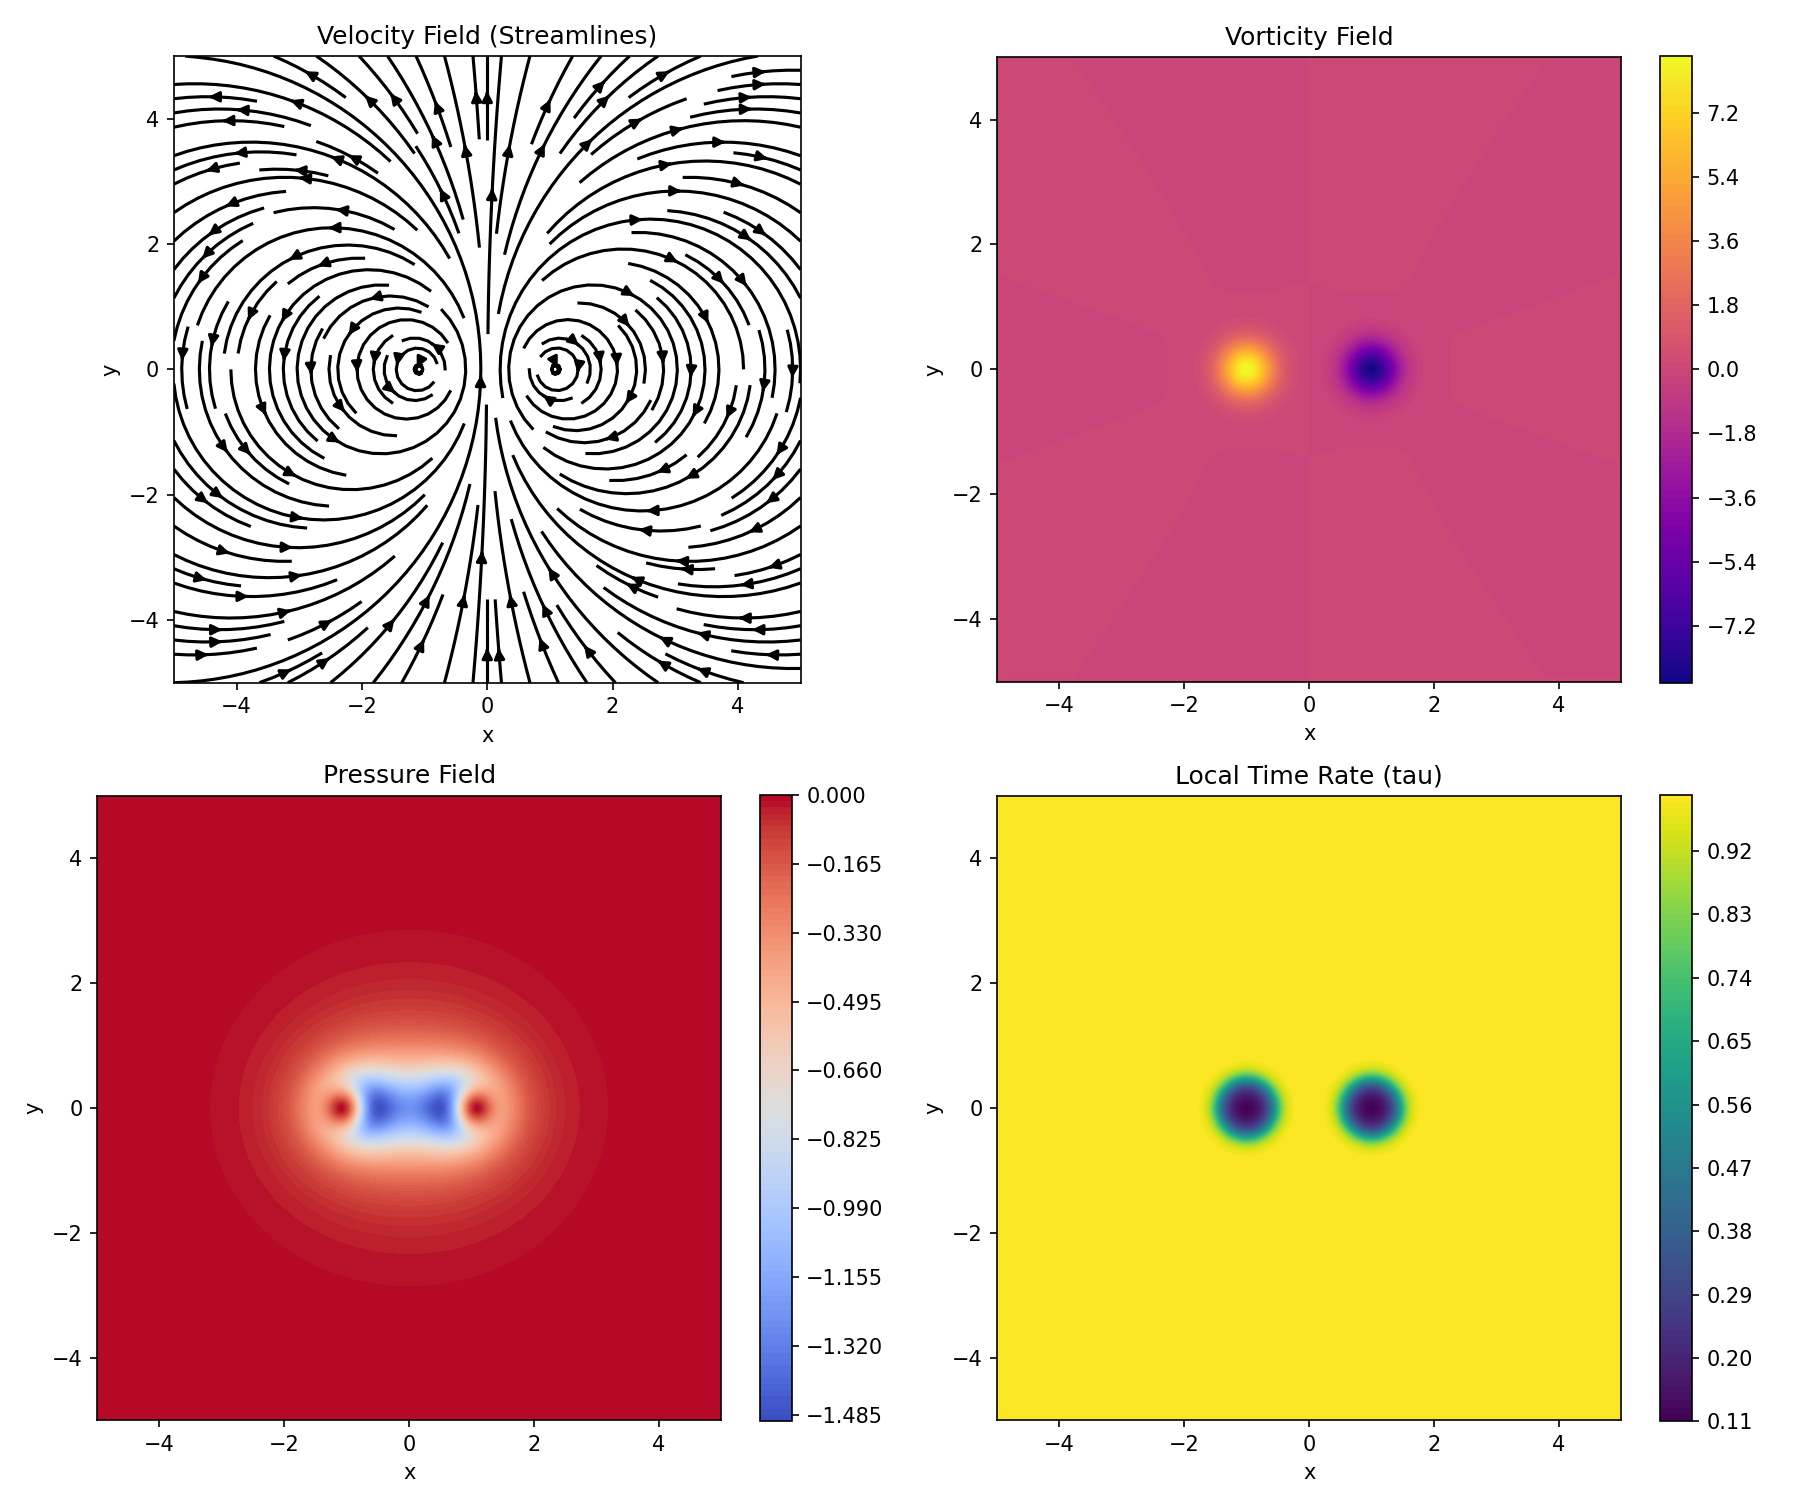
\includegraphics[width=0.85\textwidth]{streamlinesDiPole}
    \caption{Velocity streamlines, vorticity, pressure, and local time rate $\tau$ for a simulated vortex pair. The pressure minimum and time slow-down clearly align with the regions of high vorticity. This directly illustrates the æther model's central claim: time dilation follows from vortex energetics and pressure depletion.}
    \label{fig:vortexfields}
\end{figure}

\subsection{Bernoulli Flow and Local Time Depletion}

In a classical, inviscid, incompressible fluid, Bernoulli's equation describes the conservation of energy in a flow:

\begin{equation}
    \frac{1}{2} \rho_{\text{\ae}}  v^2 + p = p_0 \Rightarrow p = p_0 - \frac{1}{2} \rho_{\text{\ae}} v^2\label{eq:bernoulli}
\end{equation}

Here:
\begin{itemize}
    \item $p_0$ is the background reference pressure,
    \item $\rho_{\text{\ae}}$ is the constant æther density,
    \item $v$ is the local velocity of the æther near the vortex.
\end{itemize}

Assuming that clock rate is proportional to pressure (i.e., time slows in low-pressure regions), we relate the local clock frequency to the background as:

\begin{equation}
    \frac{f_{\text{local}}}{f_0} = 1 - \frac{\rho_{\text{\ae}} v^2}{2 p_0}\label{eq:local_clock_frequency}
\end{equation}

Hence, time dilation is:

\begin{equation}
    \frac{t_{\text{local}}}{t_0} = \left(1 - \frac{\rho_{\text{\ae}} v^2}{2 p_0}\right)^{-1}\label{eq:time_dilation}
\end{equation}

For rotational flow, with $v = \Omega r$,

\begin{equation}
    \frac{t_{\text{local}}}{t_0} = \left(1 - \frac{\rho_{\text{\ae}} \Omega^2 r^2}{2 p_0} \right)^{-1} \approx 1 + \frac{\rho_{\text{\ae}}\Omega^2 r^2}{2 p_0}\label{eq:time_dilation_rotational}
\end{equation}

This expression recovers the first-order time dilation analog if we define the dimensionless coupling:

\begin{equation}
    \frac{\rho_{\text{\ae}}}{p_0} \sim \frac{1}{c^2}\label{eq:dimensionless_coupling}
\end{equation}

This motivates the analogy to relativistic time dilation:

\begin{equation}
    \frac{t_{\text{moving}}}{t_\text{rest}} \approx 1 + \frac{v^2}{2 c^2}\label{eq:relativistic_time_dilation}
\end{equation}

\begin{figure}[htbp]
    \centering
    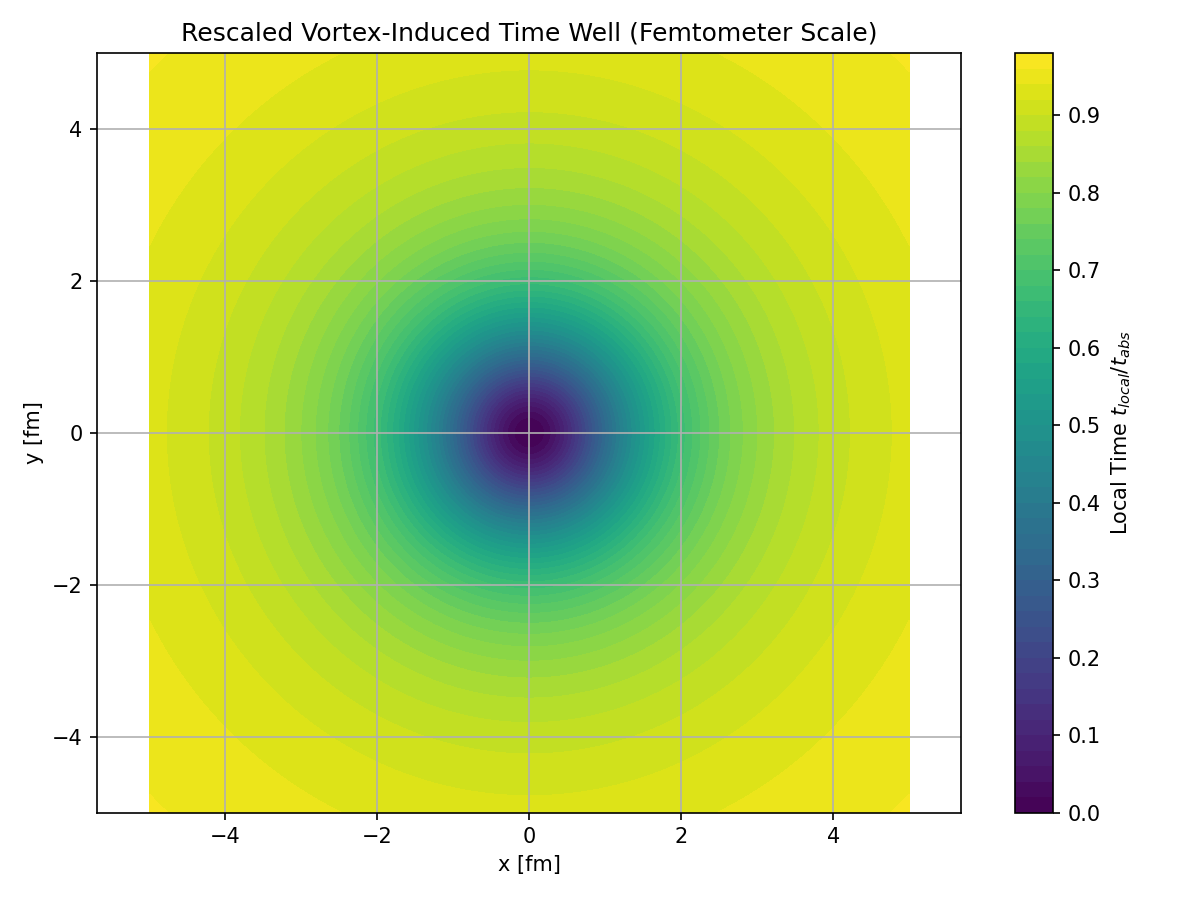
\includegraphics[width=0.8\textwidth]{RadialProfileOfLocalTimeDilation_Vortex-Induced_Time_Well}
    \caption{Schematic of a vortex-induced time well in the æther. Local time $t_{\text{local}} / t_{\text{abs}}$ is shown as a color gradient in 2D space. The central vortex region exhibits the most time slowing due to high $\Omega_k$, forming a well-like structure.}
    \label{fig:vortex_time_well}
\end{figure}


\subsection{Heuristic Knot-Based Time Modulation}

Topological vortex knots have intrinsic angular frequency $\Omega_k$, conserved due to vorticity confinement. We introduce a first-principles motivated
time dilation expression:

\begin{equation}
\frac{t_{\text{local}}}{t_{\text{abs}}} = \left(1 + \alpha \Omega_k^2 \right)^{-1}\label{eq:angular_time_dilation}
\end{equation}

where $\alpha$ is a coupling parameter with dimensions $[\alpha] = \text{s}^2$. Expanding for small $\Omega_k$:

\begin{equation}
\frac{t_{\text{local}}}{t_{\text{abs}}} \approx 1 - \alpha \Omega_k^2 + \mathcal{O}(\Omega_k^4)\label{eq:angular_time_dilation_expansion}
\end{equation}

This form parallels the Lorentz factor expansion:

\begin{equation}
\frac{t_{\text{moving}}}{t_{\text{rest}}} \approx 1 - \frac{v^2}{2 c^2}\label{eq:lorentz_time_dilation}
\end{equation}

\begin{figure}[htbp]
    \centering
    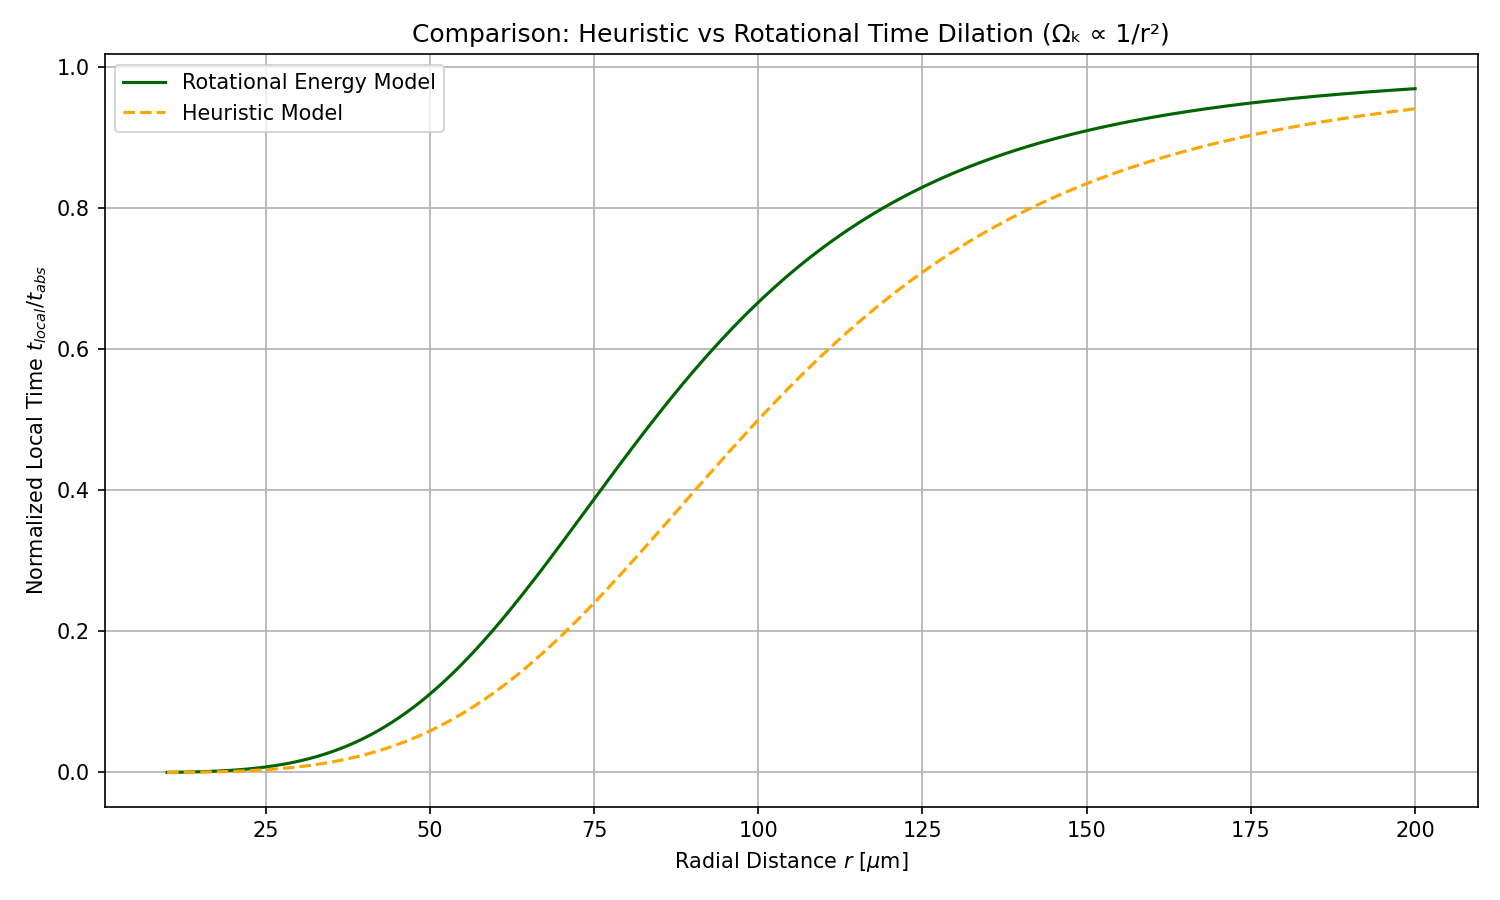
\includegraphics[width=0.8\textwidth]{RotationalVsHeuristicTimeDilation}
    \caption{\textbf{Comparison: Heuristic vs Rotational Time Dilation (\(\Omega_k \propto 1/r^2\))}.
    This graph compares two models of time modulation within the Vortex Æther framework.
    The heuristic model (green) assumes time rate reduction proportional to \((1 + \alpha \Omega_k^2)^{-1}\),
        while the rotational model (dark blue) incorporates rotational energy \(E_{\text{rot}} = \frac{1}{2} I \Omega_k^2\) and suppresses local time via
        \((1 + \frac{1}{2} \alpha I \Omega_k^2)^{-1}\). Both curves exhibit strong time dilation near the vortex core (\(r \sim 10^{-15}\) m),
        approaching absolute time flow only at extended distances. The rotational model yields a steeper suppression,
        highlighting the energetic cost of maintaining high angular momentum in fluid-based time curvature.
    }
    \label{fig:radial_time_profile}
\end{figure}

\subsection{Time Dilation from Rotational Inertia}

We now ground the heuristic form in physical energetics. For a knot with moment of inertia $I$, the rotational energy is:

\begin{equation}
E_{\text{rot}} = \frac{1}{2} I \Omega_k^2\label{eq:rotational_energy}
\end{equation}

Thus, the time dilation becomes:

\begin{equation}
\frac{t_{\text{local}}}{t_{\text{abs}}} = \left(1 + \alpha E_{\text{rot}} \right)^{-1} = \left(1 + \frac{1}{2} \alpha I \Omega_k^2 \right)^{-1}\label{eq:time_dilation_rotational_energy}
\end{equation}

This is the key result:

\begin{equation}
    \boxed{\frac{t_{\text{local}}}{t_{\text{abs}}} = \left(1 + \frac{1}{2} \alpha I \Omega_k^2 \right)^{-1}}
    \label{eq:localtime_vortex}
\end{equation}

\subsection{Summary of Model Hierarchy}

\begin{itemize}
\item Pressure-Based (Bernoulli): Time slows in low-pressure zones due to vortex velocity.
\item Heuristic Angular Model: Time slows proportionally to $\Omega_k^2$.
\item Energetic Model: Time flow depends on stored rotational energy in the knot.
\end{itemize}

These form a continuum of physical justification, culminating in a replacement of spacetime curvature with rotational æther mechanics. This establishes the VAM time dilation framework as a fluidic, topologically-conserved analog to GR.

Next, we will explore how these models correspond to GR-like metrics and rotational observers in Section II.
%\section{Entropy and Quantum Effects in the Vortex Æther Model}

The Vortex Æther Model (VAM) provides a mechanistic basis for both thermodynamic and quantum mechanical phenomena, not through postulates about abstract state spaces, but via the dynamics of knots and vortices in a superfluid æther. Two central concepts—entropy and quantization—are derived in VAM from vorticity distribution and knot topology, respectively.

\subsection{Entropy as vorticity distribution}

In thermodynamics, entropy $S$ is a measure of the internal energy distribution or disorder. In VAM, entropy does not arise as a statistical phenomenon, but from spatial variations in vorticity. For a vortex configuration $V$ the entropy is given by:

\begin{equation}
    S \propto \int_V \|\vec{\omega}\|^2 \, dV,
\end{equation}

where $\vec{\omega} = \nabla \times \vec{v}$ is the local vorticity. This means:

\begin{itemize}
    \item \textbf{More rotation = more entropy}: Regions with strong swirl contribute to increased entropy.
    \item \textbf{Thermodynamic behavior arises from vortex expansion}: With the addition of energy (heat), the vortex boundary expands, the swirl decreases and $S$ increases—analogy with gas expansion.
\end{itemize}

This interpretation connects Clausius' heat theory with æther mechanics: heat is equivalent to increased swirl spreading.

\subsection{Quantum behavior from knotted vortex structures}

Quantum phenomena such as discrete energy levels, spin, and wave-particle duality originate in VAM from topologically conserved vortex knots:

\begin{itemize}
    \item \textbf{Circulation quantization:}
    \begin{equation}
        \Gamma = \oint \vec{v} \cdot d\vec{l} = n \cdot \kappa,
    \end{equation}
    where $\kappa = h/m$ and $n \in \mathbb{Z}$ is the winding number.
    \item \textbf{Integers arise from knot topology:} The helical structure of a vortex knot (such as a trefoil) provides discrete states with certain linking numbers $L_k$.
    \item \textbf{Helicity as a spin analogue:}
    \begin{equation}
        H = \int \vec{v} \cdot \vec{\omega} \, dV,
    \end{equation}
    where $H$ is invariant under ideal flow, just as spin is conserved in quantum mechanics.
\end{itemize}

\subsection{VAM interpretation of quantization and duality}

Instead of abstract Hilbert spaces, VAM considers a particle as a stable node in the æther field. This vortex configuration has:

\begin{itemize}
    \item A \textbf{core} (nodal body) with quantum jumps (resonances).
    \item An \textbf{outer field} that acts as a wave (like the Schrödinger wave).

    \item A \textbf{helicity} that behaves as internal degrees of freedom (e.g. spin).
\end{itemize}

The wave-particle dualism thus arises from the fact that knots are both localized (core) and spread out (field).

\subsection{Summary}

VAM thus provides a coherent, fluid-mechanical origin for both:

\begin{enumerate}
    \item \textbf{Thermodynamics:} Entropy arises from swirl distribution.
    \item \textbf{Quantum mechanics:} Quantization and duality are emergent properties of knotted vortex topologies.
\end{enumerate}

This approach shows that quantum and thermodynamic phenomena are not fundamentally different, but arise from the same vortex mechanism at different scales.

\section*{Entropy as a Vorticity-Weighted Invariant}\label{sec:entropy_vorticity}

In the Vortex Æther Model (VAM), we reinterpret classical entropy as a conserved scalar related to the internal vorticity structure of knotted field regions. The classical thermodynamic differential form:
\begin{equation}
    dS = \frac{\delta Q}{T},
\end{equation}
acquires a new form when heat exchange is replaced by rotational stress input into vortex knots:
\begin{equation}
    dS = \frac{\delta \Pi_\text{rot}}{\mathcal{T}_\omega},
\end{equation}
where:
\begin{itemize}
    \item $\delta \Pi_\text{rot}$ is the differential rotational energy input to the vortex core,
    \item $\mathcal{T}_\omega$ is the effective swirl-defined temperature field,
    \item $\omega = \nabla \times \vec{v}$ is the local vorticity.
\end{itemize}
This connects thermodynamic irreversibility directly to vorticity injection and local time dilation.

\subsection*{VAM Pressure Gradients and Entropy Flow}

In VAM, pressure gradients are induced by angular momentum conservation in the æther. The classical Euler equation for incompressible inviscid flow:
\begin{equation}
    \nabla P = -\rho_\text{\ae} (\vec{v} \cdot \nabla) \vec{v},
\end{equation}
is used to express entropy production through vorticity current divergence:
\begin{equation}
    \frac{dS}{dt} = \int_V \frac{\nabla \cdot \vec{J}_\text{vortex}}{T_\omega} \, dV,
\end{equation}
where $\vec{J}_\text{vortex}$ is the swirl energy flux density. This forms the entropy production analogue of Fourier's heat conduction law within the vortex medium.

\subsection*{Thermal Expansion of Vortex Knots}

Inspired by Clausius' treatment of thermal expansion, we define a vorticity-based expansion law for knotted vortex structures:
\begin{equation}
    \Delta V_\text{knot} = \alpha_\omega V_0 \Delta T_\omega,
\end{equation}
with:
\begin{equation}
    \alpha_\omega = \frac{1}{r_c} \frac{d r_k}{d T_\omega} \sim \frac{C_e^2}{r_c k_B T_\omega},
\end{equation}
where $r_k$ is the effective knot radius, $r_c$ is the core radius, $C_e$ the core swirl velocity, and $k_B$ the Boltzmann constant. Knot inflation in VAM thus follows from ætheric heating.

\subsection*{Clausius Inequality and Helicity Dissipation}

The Clausius inequality:
\begin{equation}
    \oint \frac{\delta Q}{T} \leq 0,
\end{equation}
is reinterpreted in VAM as a constraint on helicity-induced vorticity flow:
\begin{equation}
    \oint \frac{\vec{v} \cdot d\vec{\omega}}{\mathcal{T}_\omega} \leq 0,
\end{equation}
which implies that net swirl energy circulation around closed loops is dissipative unless compensated by external ætheric drive. This underpins the irreversibility of vortex-knot interactions.

\subsection*{Carnot Efficiency in Swirl Fields}

Classical Carnot engine efficiency:
\begin{equation}
    \eta = 1 - \frac{T_C}{T_H},
\end{equation}
can be reformulated in VAM via vorticity amplitudes:
\begin{equation}
    \eta_\text{VAM} = 1 - \frac{\Omega_C^2}{\Omega_H^2},
\end{equation}
where $\Omega_H$ and $\Omega_C$ are internal angular velocities of vortex knots in high and low swirl zones. This formulation links macroscopic energy conversion directly to microscopic vorticity gradients.


%\section{Time Modulation by Rotation of Vortex Nodes}

Building on the discussion of time dilation via pressure and Bernoulli dynamics in the previous section, we now focus on the intrinsic rotation of topological vortex nodes. In the Vortex Æther Model (VAM), particles are modeled as stable, topologically conserved vortex nodes embedded in an incompressible, inviscid superfluid medium. Each node possesses a characteristic internal angular frequency $\Omega_k$, and this internal motion induces local time modulation with respect to the absolute time $\mathcal{N}$ of the æther.

Instead of warping spacetime, we propose that internal rotational energy and helicity conservation cause temporal delays analogous to gravitational redshift. In this section, these ideas are developed using heuristic and energetic arguments consistent with the hierarchy introduced in Section I.

\subsection{Heuristic and Energetic Derivation}

We start by proposing a rotationally induced time dilation formula based on the internal angular frequency of the vortex node:

\begin{equation}
    \frac{d\tau}{d\mathcal{N}} = \left(1 + \beta \Omega_k^2 \right)^{-1}
    \quad \text{(Chronos-Time slowdown due to internal vortex rotation)}
    \label{eq:chronos_swirl_slowdown}
\end{equation}

where:

\begin{itemize}
    \item $\tau$ is the local Chronos-Time (proper time experienced by the vortex structure),
    \item $\mathcal{N}$ is the absolute Aithēr-Time (universal causal background),
    \item $\Omega_k$ is the mean core angular frequency,
    \item $\beta$ is a coupling coefficient with units $[\beta] = \mathrm{s}^2$.
\end{itemize}

For small angular velocities we obtain a first-order expansion:

\begin{equation}
    \frac{d\tau}{d\mathcal{N}} \approx 1 - \beta \Omega_k^2 + \mathcal{O}(\Omega_k^4)
\end{equation}

This mirrors the low-velocity expansion of the Lorentz factor in special relativity:
\begin{equation}
    \frac{t_\text{moving}}{t_\text{rest}} \approx 1 - \frac{v^2}{2c^2}
\end{equation}

We observe that internal rotation in VAM induces time dilation just as relative motion does in SR—yet from internal dynamics, not frame-relative velocity.

To support this with physical grounding, we connect time dilation to rotational energy. Suppose the vortex node has an effective moment of inertia $I$. The rotational energy becomes:

\begin{equation}
    E_\text{rot} = \frac{1}{2} I \Omega_k^2
\end{equation}

This leads to the energetic expression:
\begin{equation}
    \frac{d\tau}{d\mathcal{N}} = \left(1 + \beta E_\text{rot} \right)^{-1}
    = \left(1 + \frac{1}{2} \beta I \Omega_k^2 \right)^{-1}
\end{equation}

This equation parallels the pressure-induced time modulation derived from Bernoulli dynamics earlier in the paper and supports the concept of rotational time wells induced by internal energy storage.

\begin{tcolorbox}[colback=gray!5, colframe=black!70, sharp corners=southwest, title=Temporal Mapping for Vortex Nodes]
In the Vortex Æther Model:
\begin{itemize}
    \item \( \mathcal{N} \) — \textbf{Aithēr-Time:} Universal causal flow (background time),
    \item \( \tau \) — \textbf{Chronos-Time:} Local inertial time along vortex evolution,
    \item \( S(t) \) — \textbf{Swirl Clock:} Phase memory due to internal angular rotation.
\end{itemize}
Equation~\eqref{eq:chronos_swirl_slowdown} captures how increasing swirl leads to slower proper time relative to the ætheric background.
\end{tcolorbox}

\subsection{Topological and Physical Justification}

Topological vortex nodes are characterized not only by rotation, but also by helicity:
\begin{equation}
    H = \int \vec{v} \cdot \vec{\omega} \, d^3x
\end{equation}

Helicity is a conserved quantity in ideal fluids and encodes the topological linkage and twist of vortex lines. Thus, the rotation frequency $\Omega_k$ becomes a signature of the knot’s identity and energy state.

Higher $\Omega_k$ values produce stronger swirl wells and deeper pressure minima, resulting in longer internal durations per unit $\mathcal{N}$. This time dilation is interpreted as a reduction in Chronos-Time, not as a change in spacetime geometry.

Each particle is a topological vortex knot, where:
\begin{itemize}
    \item \textbf{Charge} maps to chirality and rotational direction,
    \item \textbf{Mass} maps to total vortex energy (and inertia),
    \item \textbf{Spin} maps to knot helicity and winding structure.
\end{itemize}

Knot type (e.g. Hopf, Trefoil) determines its stability and energetic minimum.

This model:

\begin{itemize}
    \item Attributes temporal modulation to conserved rotational energy,
    \item Requires no relativistic reference frames,
    \item Embeds all time shifts within the æther’s causal substrate $\mathcal{N}$,
    \item Provides a direct fluid-mechanical analogue to gravitational redshift.
\end{itemize}

\textbf{In summary:} Vortex-induced time dilation in VAM is governed by the equation
\[
    \frac{d\tau}{d\mathcal{N}} = \left(1 + \beta \Omega_k^2 \right)^{-1}
\]
showing that Chronos-Time slows as internal vortex angular velocity increases — a purely mechanical, topologically-grounded origin of time dilation, replacing the abstract spacetime curvature of general relativity.

%\input{Swirl_Clocks/04_Proper_Time_for_a_Rotating_Observer_in_Æther_Flow}
%\section{Kerr-like Time Adjustment Based on Vorticity and Circulation}

To complete the analogy between general relativity (GR) and the Vortex Æther Model (VAM), we derive a time modulation expression that mimics the redshift and frame-dragging structure of the Kerr solution. In GR, the Kerr metric describes the curved spacetime near a rotating mass, leading to gravitational time dilation and frame-dragging. In VAM, similar effects arise from local vorticity intensity and circulation in a flat æther, relative to absolute time \( \mathcal{N} \).

\subsection{General Relativistic Kerr Redshift Structure}

In the GR-Kerr metric, the proper time \( d\tau_{\text{GR}} \) for an observer is slowed by both mass-energy and angular momentum:

\begin{equation}
    t_{\text{adjusted}} = \Delta t \cdot \sqrt{1 - \frac{2GM}{rc^2} - \frac{J^2}{r^3c^2}}
    \label{eq:Kerr_time_dilation}
\end{equation}

\noindent with:
\begin{itemize}
    \item \( M \): mass,
    \item \( J \): angular momentum,
    \item \( r \): radius,
    \item \( G \): gravitational constant,
    \item \( c \): speed of light.
\end{itemize}

\subsection{VAM Analogy via Vorticity and Circulation}

In VAM, we substitute GR's mass and angular momentum terms with vorticity-based quantities:

\begin{itemize}
    \item \( \langle \omega^2 \rangle \): spatially averaged squared vorticity (linked to energy density),
    \item \( \kappa \): total circulation (encoding angular momentum).
\end{itemize}

The mapping becomes:

\begin{equation}
    \begin{aligned}
        \frac{2GM}{rc^2} &\rightarrow \frac{\gamma \langle \omega^2 \rangle}{r c^2}, \\
        \frac{J^2}{r^3 c^2} &\rightarrow \frac{\kappa^2}{r^3 c^2}
    \end{aligned}
    \label{eq:Kerr_replacements}
\end{equation}

\noindent where \( \gamma \) is a coupling constant derived from æther properties.

The VAM redshift-adjusted external time \( \bar{t} \) observed at infinity becomes:

\begin{equation}
    \boxed{
        \frac{d\tau}{d\bar{t}} = \sqrt{1 - \frac{\gamma \langle \omega^2 \rangle}{r c^2} - \frac{\kappa^2}{r^3 c^2}}
    }
    \label{eq:Kerr_time_dilation_ae}
\end{equation}

This replaces the geometric redshift of GR with a purely fluid-based expression. In the absence of vorticity and circulation, \( \tau \to \bar{t} \), recovering flat time flow. In this figure:
\begin{itemize}
    \item $\langle \omega^2 \rangle$ plays the role of energy density that produces gravitational redshift,
    \item $\kappa$ represents angular momentum that generates temporal frame-dragging,
    \item The equation reduces to a flat æther time ($t_\text{adjusted} \to \Delta t$) when both terms vanish.

\end{itemize}

\subsection*{Hybrid Frame-Dragging Angular Velocity in VAM}

Frame-dragging in VAM emerges from vortex coupling to surrounding flow. The effective angular velocity imposed on surrounding regions becomes:

\begin{equation}
    \omega_\text{drag}^\text{VAM}(r) =
    \frac{4 G m}{5 c^2 r} \cdot \mu(r) \cdot \Omega(r)
\end{equation}

\noindent with a scale-dependent interpolation factor:

\begin{equation}
    \mu(r) =
    \begin{cases}
        \frac{r_c C_e}{r^2}, & r < r_\ast \quad \text{(quantum/vortex regime)} \\
        1, & r \geq r_\ast \quad \text{(macroscopic limit)}
    \end{cases}
\end{equation}

This allows for continuity between quantum vortex-induced frame-dragging and classical GR effects.
where:
\begin{itemize}
    \item \( r_c \) is the radius of the vortex core,
    \item \( C_e \) is the tangential velocity of the vortex core,
    \item \( r_\ast \sim 10^{-3} \, \text{m} \) is the transition radius between microscopic and macroscopic regimes.
\end{itemize}

This formulation provides continuity with GR predictions for celestial bodies, while allowing VAM-specific predictions for elementary particles and subatomic vortex structures.

\subsection*{Gravitational Redshift from Vortex Core Rotation}

Gravitational redshift in VAM arises from tangential velocity \( v_\varphi = \Omega(r) \cdot r \) at the vortex periphery. The redshift becomes:

\begin{equation}
    z_\text{VAM} = \left( 1 - \frac{v_\varphi^2}{c^2} \right)^{-\frac{1}{2}} - 1
\end{equation}

This defines the deviation of external clock time \( \bar{t} \) from Chronos-Time \( \tau \) near the vortex. As \( v_\varphi \to c \), the local observer experiences time freeze:

\[
    \lim_{v_\varphi \to c} z_\text{VAM} \to \infty
\]

where:
\begin{itemize}
    \item \( v_\phi = \Omega(r) \cdot r \) is the tangential velocity due to local rotation,
    \item \( \Omega(r) \) is the angular velocity at the measurement beam \( r \),
    \item \( c \) is the speed of light in vacuum.

\end{itemize}

This expression reflects the change in time perception caused by local rotational energy, replacing the curvature-based gravitational potential \( \Phi \) of general relativity with a velocity field term. It becomes equivalent to the GR Schwarzschild redshift for low \( v_\phi \) and diverges as \( v_\phi \rightarrow c \), which provides a natural limit to the evolution of the local frame:

\subsection*{Time Dilation Models in VAM}

\paragraph{Velocity-based time dilation (outer observer):}

\begin{equation}
    \frac{d\tau}{d\bar{t}} =
    \sqrt{1 - \frac{\Omega^2 r^2}{c^2}} = \sqrt{1 - \frac{v_\varphi^2}{c^2}}
\end{equation}

\paragraph{Energy-based time dilation (core structure):}

\begin{equation}
    \frac{d\tau}{d\mathcal{N}} =
    \left( 1 + \frac{1}{2} \cdot \beta \cdot I \cdot \Omega^2 \right)^{-1}
\end{equation}

\noindent where:

- \( \mathcal{N} \) is Aithēr-Time,
- \( \tau \) is Chronos-Time,
- \( I = \frac{2}{5} m r^2 \), \( \beta = \frac{r_c^2}{C_e^2} \).

This dual-model captures both peripheral redshift (via \( \bar{t} \)) and intrinsic time contraction (via \( \mathcal{N} \)).


In the Vortex Æther Model (VAM), local time dilation is interpreted as the modulation of absolute time by internal vortex dynamics, not by spacetime curvature. Depending on the system scale, two physically based formulations are used:

\paragraph{1. Time dilation based on velocity fields}

This model relates the local time flow to the tangential speed of the rotating ætheric structure (vortex node, planet or star):

\begin{equation}
    \frac{d\tau}{d\bar{t}} =
    \sqrt{1 - \frac{v_\phi^2}{c^2}} =
    \sqrt{1 - \frac{\Omega^2 r^2}{c^2}} \quad \text{(external observer)}
\end{equation}

whereby:
\begin{itemize}
    \item \( v_\phi = \Omega \cdot r \) is the tangential speed,
    \item \( \Omega \) is the angular velocity at radius \( r \),
    \item \( c \) is the speed of light.
\end{itemize}

This expresses how a local observer's Chronos-Time $\tau$ slows down relative to a distant clock, as seen in:
\begin{itemize}
\item redshift measurements
\item external clocks
\item comparisons to signals emitted from afar.
\end{itemize}



\paragraph{2. Time dilation based on rotational energy}

On large scales or with high rotational inertia, time dilation arises from stored rotational energy, leading to:

\begin{equation}
   \frac{d\tau}{d\mathcal{N}} = \left(1 + \frac{1}{2} \cdot \beta \cdot I \cdot \Omega^2 \right)^{-1} \quad \text{(background time)}
\end{equation}

with:
\begin{itemize}
    \item \( I = \frac{2}{5} m r^2 \): moment of inertia for a uniform sphere,
    \item \( \beta = \frac{r_c^2}{C_e^2} \): coupling constant of vortex-core dynamics,
    \item \( m \) is the mass of the object.
\end{itemize}

This describes how the local vortex structure's internal clock slows due to stored rotational energy, measured relative to the universal causal background $\mathcal{N}$ — i.e., the absolute time field of the æther. It reflects internal modulation of a structure's proper time due to internal dynamics — not relative motion.


\subsection*{Temporal Ontology Integration Summary}

\begin{itemize}
    \item \( \mathcal{N} \) — Universal Aithēr-Time,
    \item \( \bar{t} \) — External Clock Time (distant observer),
    \item \( \tau \) — Local Chronos-Time (experienced time),
    \item \( S(t) \) — Swirl Clock phase evolution,
    \item \( T_v \) — Vortex Proper Time along internal loop.
\end{itemize}

The combined time dilation structure can be captured schematically as:

\begin{equation}
\boxed{
\frac{d\tau}{d\bar{t}} =
\sqrt{1 - \frac{\gamma \langle \omega^2 \rangle}{r c^2} - \frac{\kappa^2}{r^3 c^2}} \cdot
\left(1 + \frac{1}{2} \beta I \Omega^2 \right)^{-1}
}
\label{eq:VAM_combined_time_dilation}
\end{equation}


\paragraph{Interpretation}

These models imply that time slows down in regions of high local rotational energy or vorticity, consistent with gravitational time dilation effects in GR. In VAM, however, these effects arise exclusively from the internal dynamics of the æther flow, under flat 3D Euclidean geometry and absolute time.

\subsection*{Model Scope and Outlook}

These expressions assume:F
- Ideal incompressible superfluid,
- Irrotational flow outside vortex cores,
- Neglect of turbulence and boundary-layer effects.

Appendix~\ref{sec:appendix:7} provides detailed derivations of energy transfer across interacting vortex layers. In future work, quantized circulation and ætheric boundary effects may refine these models further.

%\section{Unified Framework and Synthesis of Time Dilation in VAM}

This section unifies all time dilation mechanisms developed throughout this work under the Vortex Æther Model (VAM). Instead of relying on spacetime curvature, VAM attributes temporal effects to classical fluid dynamics, rotational energy, and topological vorticity embedded in an absolute superfluid medium.

\subsection{Hierarchical Structure of Time Dilation Mechanisms}

Each mechanism introduced in previous sections corresponds to a physically distinct layer of time modulation in the æther:

\begin{enumerate}
    \item \textbf{Bernoulli-Induced Time Depletion:} Time slows down in low-pressure regions due to vortex-induced kinetic fields. When \( \rho_\text{\ae} / p_0 \sim 1/c^2 \), the Bernoulli velocity field reproduces SR-like time dilation.

    \item \textbf{Heuristic Angular Frequency Dilation:} A first-order expansion in internal angular frequency \( \Omega_k \) yields:
    \[
        \frac{d\tau}{d\mathcal{N}} \approx 1 - \beta \Omega_k^2
    \]
    mimicking Lorentz factor expansions.

    \item \textbf{Energetic Time Dilation from Rotational Inertia:}
    \[
        \boxed{\frac{d\tau}{d\mathcal{N}} = \left(1 + \frac{1}{2} \beta I \Omega_k^2 \right)^{-1}}
    \]
    based on rotational energy of a vortex node.

    \item \textbf{Proper Time in a Vortex Flow Field:}
    \[
        \boxed{
        \left( \frac{d\tau}{d\bar{t}} \right)^2 = 1 - \frac{1}{c^2}(v_r + r \Omega_k)^2
        }
    \]
    deriving GR-like behavior from tangential + radial æther velocity.

    \item \textbf{Kerr-Like Redshift with Vorticity and Circulation:}
    \[
        \boxed{
        \frac{d\tau}{d\bar{t}} = \sqrt{1 - \frac{\gamma \langle \omega^2 \rangle}{r c^2} - \frac{\kappa^2}{r^3 c^2}}
        }
    \]
    fluid-based replacement for GR Kerr redshift structure.
\end{enumerate}

Together, these span from microscale vortex energetics to macroscale rotation and redshift analogies, offering a complete and experimentally accessible formulation of time dilation in a flat 3D ætheric medium.

\subsection{Time as a Vorticity-Derived Observable}

Across all levels, time modulation in VAM reduces to local energetics:
\begin{itemize}
    \item Pressure, velocity, and swirl induce local slowing of Chronos-Time \( \tau \).
    \item Core angular frequency \( \Omega_k \) governs vortex Proper Time \( T_v \).
    \item Accumulated swirl phase \( S(t) \) encodes vortex history and coherence.
    \item Background evolution proceeds along absolute Aithēr-Time \( \mathcal{N} \).
\end{itemize}

Time becomes an emergent fluid quantity, shaped by:
\begin{itemize}
    \item Kinetic flow energy,
    \item Rotational inertia,
    \item Vorticity intensity \( \langle \omega^2 \rangle \),
    \item Topologically conserved circulation \( \kappa \).
\end{itemize}

This leads to a boxed synthesis:

\begin{equation}
\boxed{
\frac{d\tau}{d\bar{t}} =
\sqrt{1 - \frac{\gamma \langle \omega^2 \rangle}{r c^2} - \frac{\kappa^2}{r^3 c^2}} \cdot
\left(1 + \frac{1}{2} \beta I \Omega_k^2 \right)^{-1}
}
\label{eq:VAM_final_time_dilation}
\end{equation}

\subsection{Experimental Implications and Prospects}

The following systems may be used to validate aspects of this framework:
\begin{itemize}
    \item Rotating superfluid droplets (helium-II, BECs),
    \item Plasma vortex lifters and EHD propulsion systems,
    \item Magneto-fluidic toroidal devices or photonic vortex rings,
    \item Rotating dielectric experiments with Swirl Clock analogs.
\end{itemize}

Future directions:
\begin{itemize}
    \item Measure vortex-induced clock drift in rotating superfluids.
    \item Apply to neutron star precession, Lense–Thirring analogs.
    \item Derive feedback models of interacting vortex clocks in multi-body ætheric networks.
\end{itemize}

\subsection{Conceptual Challenges and Reception}

\textbf{Assumptions:}
\begin{itemize}
    \item Existence of absolute time \( \mathcal{N} \),
    \item Incompressible, inviscid superfluid æther,
    \item Structured vortex knots as physical particles.
\end{itemize}

\textbf{Resistance:}
\begin{itemize}
    \item Contradicts mainstream relativistic orthodoxy,
    \item Requires reinterpretation of spacetime as emergent, not fundamental.
\end{itemize}

\subsection{Paths to Scientific Rigor and Acceptance}

\begin{itemize}
    \item \textbf{Testable predictions:} where VAM diverges from GR.
    \item \textbf{Integration:} recover GR/QM limits for boundary cases.
    \item \textbf{Redefinition:} modern æther = structured field, not rigid ether.
    \item \textbf{Open review:} encourage formal peer critique and simulation.
    \item \textbf{Clarity:} maintain symbolic and dimensional transparency.
\end{itemize}

\subsection{Concluding Perspective}

The Vortex Æther Model (VAM) replaces the geometry of curved spacetime with a dynamic, energetic æther in which time flows at different rates due to vorticity and circulation. This provides a coherent, layered framework in which relativistic effects arise naturally from fluid variables, with internal clocks modulated by swirl dynamics and structure-preserving topology.

As a next step, a Lagrangian formalism incorporating \( \tau \), \( T_v \), \( S(t) \), and \( \mathcal{N} \) can unify gravity, quantum behavior, and thermodynamics under a common ætheric field theory.


%\section{Applications of VAM to Quantum and Nuclear Processes}
\label{sec:LENR_QED}

\subsection*{LENR via Resonance Tunneling and Temporal Modulation}

In the Vortex Æther Model (VAM), gravitational decay due to local vorticity temporarily lowers the Coulomb barrier, shifting the rate of local \emph{Chronos-Time} (\(\tau\)) and inducing a transient \emph{Kairos Moment} (\(\kappa\))—a topological and energetic bifurcation—where irreversible tunneling becomes energetically favorable:

\begin{equation}
    V_\text{Coulomb} = \frac{Z_1 Z_2 e^2}{4\pi \varepsilon_0 r}, \quad
    \Delta P = \frac{1}{2} \rho_\text{\ae} r_c^2 (\Omega_1^2 + \Omega_2^2)
\end{equation}

Resonance occurs when:

\begin{equation}
    \Delta P \geq \frac{Z_1 Z_2 e^2}{4\pi \varepsilon_0 r_t^2}
\end{equation}

Rather than invoking purely probabilistic tunneling, VAM attributes the transition to real pressure gradients in a structured æther. This echoes the causal flow picture of Holland~\cite{holland1993quantum}, in which trajectories are guided by underlying fields rather than collapsed by observation.

\subsection*{Resonant Ætheric Tunneling and LENR in VAM}

LENR events are thus reinterpreted as phase-locked vortex interactions within the æther, where pressure minima—caused by Bernoulli-type deficits from vortex swirl—transiently erase the Coulomb barrier~\cite{Barcelo2011, volovik2003}.

The classical Coulomb repulsion between two nuclei is:

\begin{equation}
    V_\text{Coulomb}(r) = \frac{Z_1 Z_2 e^2}{4\pi \varepsilon_0 r}
\end{equation}

In VAM, two rotating vortex nodes near \( r \sim 2r_c \) generate a pressure drop:

\begin{equation}
    \Delta P = \frac{1}{2} \rho_\text{\ae} r_c^2 (\Omega_1^2 + \Omega_2^2)
\end{equation}

The effective potential becomes:

\begin{equation}
    V_\text{eff}(r) = V_\text{Coulomb}(r) - \Phi_\omega(r)
\end{equation}

with the vorticity (eddy) potential defined as:

\begin{equation}
    \Phi_\omega(r) = \gamma \int \frac{|\vec{\omega}(r')|^2}{|\vec{r} - \vec{r}'|} \, d^3r',
    \quad \text{where} \quad \gamma = G \rho_\text{\ae}^2
\end{equation}

Resonant tunneling occurs when:

\begin{equation}
    \frac{1}{2} \rho_\text{\ae} r_c^2 (\Omega_1^2 + \Omega_2^2) \geq \frac{Z_1 Z_2 e^2}{4\pi \varepsilon_0 r_t^2}
\end{equation}

This process manifests as a local disruption in the vortex-phase evolution \(S(t)\), corresponding to a \emph{Kairos Moment} (\(\kappa\))—a non-reversible, quantized transition in the topology of the field structure. The tunneling does not proceed by stochastic amplitude leakage, but via real-time phase-coherent alignment of swirl dynamics.

\paragraph{Temporal Interpretation:}

At the critical separation \(r_t\), the reduction in \(\bar{t}\)-duration (as seen by external observers) corresponds to a locally accelerated evolution in the Swirl Clock \(S(t)\), while the internal Chronos-Time \(\tau\) of the system undergoes inflection. This manifests as a moment of energetic coincidence across temporal layers, enabling otherwise forbidden nuclear transitions.

This mechanism offers a testable, topologically anchored alternative to conventional quantum tunneling, and may help explain anomalous energy release observed in some LENR experiments~\cite{Storms2021}.
\subsection*{VAM Quantum Electrodynamics (QED) Lagrangian}

In the Vortex Æther Model (VAM), the interaction between vortex structures and electromagnetic fields emerges from the helical motion of knotted vortex cores. These structures induce localized vector potentials in the surrounding æther, and thus replace the conventional QED framework with a topological fluid-dynamic interpretation.

The VAM analog of the standard QED Lagrangian is:

\begin{equation}
    \mathcal{L}_\text{VAM-QED} =
    \bar{\psi} \left[ i \gamma^\mu \partial_\mu
                   - \gamma^\mu \left( \frac{C_e^2 r_c}{\lambda_c} \right) A_\mu
                   - \left( \frac{8\pi \rho_\text{\ae} r_c^3 \, \text{Lk}}{C_e} \right) \right] \psi
    - \frac{1}{4} F_{\mu\nu} F^{\mu\nu}
\end{equation}

In this formulation:
\begin{itemize}
    \item The \textbf{mass term} emerges from the topological helicity (linking number Lk) of connected vortex cores, interpreted as a geometric invariant tied to conserved Vortex Proper Time \( T_v \)~\cite{volovik2003}.
    \item The \textbf{electromagnetic coupling} arises not from a fundamental charge, but from ætheric circulation that induces the gauge potential \( A_\mu \).
    \item The \textbf{field tensor} \( F_{\mu\nu} \) remains unchanged and still encodes the curl of the velocity field—interpreted now as the rotation of the superfluid æther medium rather than of spacetime.
\end{itemize}

This Lagrangian directly couples spinor fields to ætheric vorticity and replaces the usual constants \( m \) and \( q \) with emergent expressions involving core radius \( r_c \), tangential velocity \( C_e \), and topological helicity \( \text{Lk} \). Mass and charge thus arise as vortex-induced effective quantities rather than as primitive attributes.

The resulting Euler–Lagrange equation yields:

\begin{equation}
    \boxed{
    \left( i \gamma^\mu \partial_\mu
         - \gamma^\mu q_\text{vortex} A_\mu
         - M_\text{vortex}
    \right)\psi = 0
    }
\end{equation}

This is structurally identical to the Dirac equation, but its parameters originate in the vortex configuration of the æther. Thus, VAM reinterprets the origin of inertial mass and electric charge as byproducts of topological flow in a superfluid medium~\cite{Barcelo2011, volovik2003}.

\begin{figure}[H]
    \centering
    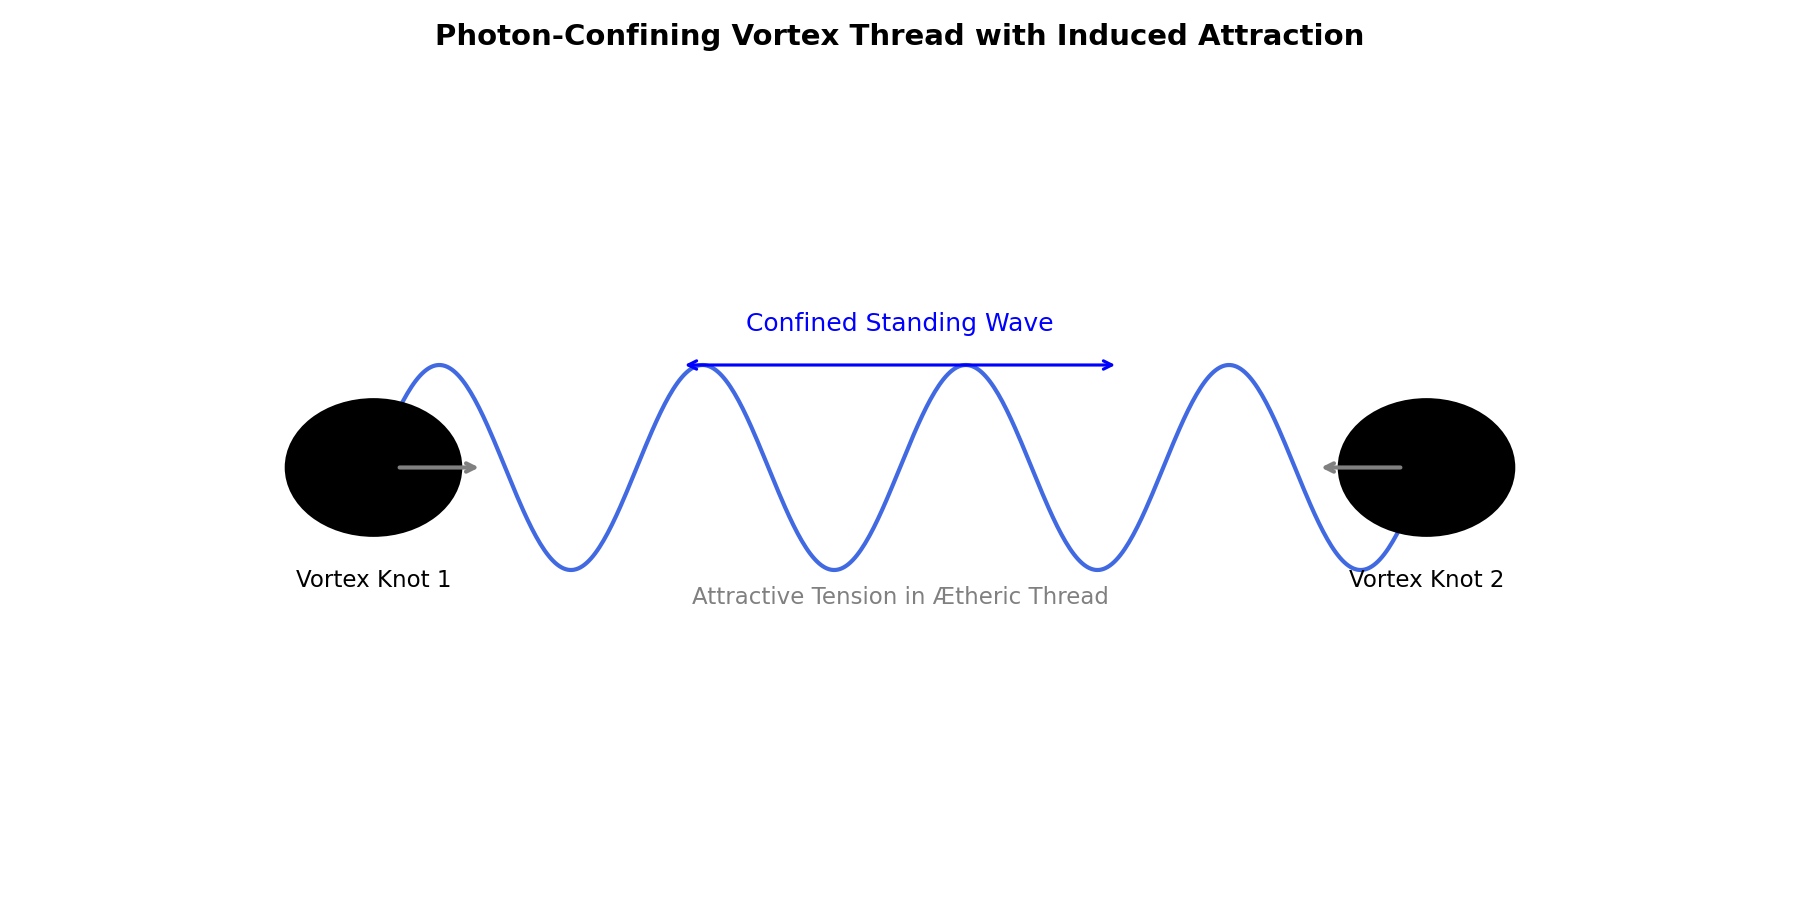
\includegraphics[width=0.85\textwidth]{images/08-Photon-ConfiningVortexThreadGravitation}
    \caption{Photon confinement and guidance along vortex threads in the æther. This visualizes the VAM interpretation of electromagnetic propagation, where the photon exhibits localized trajectory bending and resonance around structured vortex lines. The confinement arises naturally from topological pressure minima and circulating æther flow, replacing the abstract field representation with a tangible vortex-based channel.}
    \label{fig:photon_confine}
\end{figure}

\section{Emergent Bohr Radius from Vortex Swirl Pressure}

To demonstrate how atomic structure arises in the Vortex \AE ther Model (VAM), we derive the Bohr radius from first principles using fluid dynamic forces. In this model, the electron is a knotted vortex core circulating with tangential speed $C_e$, and atomic stability arises from pressure gradients and swirl quantization.

\subsection*{Standard Quantum Bohr Radius}

In canonical quantum mechanics, the Bohr radius is the radius of the lowest energy orbit in the hydrogen atom, balancing centripetal and Coulomb forces:
\begin{equation}
    a_0 = \frac{4\pi \varepsilon_0 \hbar^2}{m_e e^2}
\end{equation}

\subsection*{Swirl Dynamics and Force Balance in VAM}

In VAM, swirl flow replaces wavefunction orbitals. The tangential velocity at radius $r$ due to vortex circulation is:
\begin{equation}
    v_\phi(r) = \frac{\Gamma}{2\pi r}, \quad \text{with} \quad \Gamma = 2\pi r_c C_e
\end{equation}
Thus:
\begin{equation}
    v_\phi(r) = \frac{r_c C_e}{r}
\end{equation}

Force balance between centrifugal and Coulomb-like tension in the \ae ther gives:
\begin{equation}
    \frac{m_e v_\phi^2}{r} = \frac{e^2}{4\pi \varepsilon_0 r^2}
\end{equation}

Substituting:
\begin{equation}
    \frac{m_e (r_c C_e)^2}{r^3} = \frac{e^2}{4\pi \varepsilon_0 r^2}
\end{equation}
Multiply both sides by $r^3$ and solve for $r$:
\begin{equation}
    a_0 = \frac{4\pi \varepsilon_0 m_e r_c^2 C_e^2}{e^2}
\end{equation}

\subsection*{Numerical Evaluation}

\begin{align*}
    \varepsilon_0 &= 8.854187817 \times 10^{-12}~\si{F/m} \\
    m_e &= 9.1093837015 \times 10^{-31}~\si{kg} \\
    r_c &= 1.40897017 \times 10^{-15}~\si{m} \\
    C_e &= 1.09384563 \times 10^6~\si{m/s} \\
    e &= 1.602176634 \times 10^{-19}~\si{C}
\end{align*}

Substituting, we recover:
\[
    a_0 \approx 5.29 \times 10^{-11}~\si{m}
\]

\subsection*{Swirl Clock Quantization and Stable Orbits}

This equilibrium radius coincides with the \textbf{first harmonic phase-lock} of the Swirl Clock $S(t)$, where the angular phase of the circulating vortex completes a stable winding over vortex proper time $T_v$. Each quantized orbit corresponds to a resonance in $S(t)$ such that:
\[
    S(t) = 2\pi n, \quad n \in \mathbb{Z}^+
\]
\[
    \Rightarrow \Omega_n T_v = 2\pi n \quad \text{(Quantized vortex phase winding)}
\]

Thus, the Bohr radius is the radial location where a full swirl-phase cycle completes within a stable energetic well. This is not arbitrary but reflects \ae ther-tuned topological resonance, producing \textbf{standing swirl modes} tied to the vortex knot's structure.

\subsection*{Temporal Interpretation}

\begin{itemize}
    \item Local \textbf{Chronos-Time} $\tau$ inside the vortex slows relative to the external $\bar{t}$ due to swirl-induced dilation:
    \[ \frac{d\tau}{d\bar{t}} = \sqrt{1 - \frac{v_\phi^2}{c^2}} \]
    \item The Bohr radius marks the radius where $T_v$ and $\tau$ evolve stably under a quantized $S(t)$, enabling persistent atomic states.
\end{itemize}

\subsection*{Interpretation}

\begin{equation}
    \boxed{
        \text{Bohr radius in VAM} =
        \text{Stable tidal resonance of swirl pressure in a vortex-induced \ae ther cavity}
    }
\end{equation}

This reproduces quantum mechanical results through fluid analogs and structured vortex flows. No probability waves are invoked---only energetically balanced circulation under absolute time evolution.

\subsection*{Future Work}

\begin{itemize}
    \item Generalize to multi-electron atoms via nested swirl clock harmonics.
    \item Derive fine structure constant from coupling between $C_e, r_c, \rho_\text{\ae}$.
    \item Quantize transitions as topological bifurcations in $S(t)$ --- marking \textbf{Kairos Moments} $\kappa$.
\end{itemize}

%\section{VAM Vorticity Scattering Framework (inspired by elastic theory)}

\subsection{Governing equations of VAM Vorticity dynamics}

\subsubsection*{Vorticity transport equation (linearized form)}

In the Vortex Æther Model (VAM), the dynamics of the vorticity field \(\vec{\omega} = \nabla \times \vec{v}\) is governed by the Euler equation and the associated vorticity form:

\[
    \frac{\partial \omega_i}{\partial t} + v_j \partial_j \omega_i = \omega_j \partial_j v_i
\]

This nonlinear structure implies vortex deformation by stretching and advection. For small perturbations \(\delta\omega\) near a background vortex node field \(\omega^{(0)}\) linearization yields:

\[
    \frac{\partial (\delta \omega_i)}{\partial t} + v_j^{(0)} \partial_j (\delta \omega_i) \approx \omega_j^{(0)} \partial_j (\delta v_i)
\]

Define the linear response operator of VAM \(\mathcal{L}_{ij}\):

\[
    \mathcal{L}_{ij} \, \delta v_j(\vec{r}) = \delta F_i^\text{vortex}(\vec{r})
\]

\subsubsection*{Green Tensor Vorticity Equation}

\[
    \mathcal{L}_{ij} \, \mathcal{G}_{jk}(\vec{r}, \vec{r}') = -\delta_{ik} \, \delta(\vec{r} - \vec{r}')
\]

The induced velocity field \(v_i\) of a source vortex force \(F_k(\vec{r}')\) is then:

\[
    v_i(\vec{r}) = \int \mathcal{G}_{ik}(\vec{r}, \vec{r}') \, F_k^\text{vortex}(\vec{r}') \, d^3 r'
\]

\subsection{Vortex filament interaction}
Interactions arise from exchange of vortex force or Reconnections between vortex filaments:
\begin{itemize}
    \item Attractive when filaments reinforce the circulation (parallel)
    \item Repulsive when filaments cancel each other out (antiparallel)
    \item Interaction strength:
\end{itemize}
\begin{equation}
    \vec{F}_\text{int} = \beta \cdot \kappa_1 \kappa_2 \cdot \frac{\vec{r}_{12} \times (\vec{v}_1 - \vec{v}_2)}{|\vec{r}_{12}|^3}\label{eq:interaction_strength}
\end{equation}
Where \(\kappa_i\) are the circulations of filaments and \(\vec{r}_{12}\) is the vector between them.

\subsection{Thermodynamic \& quantum behavior of vorticity fluctuations}
\begin{itemize}
    \item Entropy \(\leftrightarrow\) volume of vortex expansion or knot deformation
    \item Quantum transitions \(\leftrightarrow\) topological reconnection events
    \item Zero-point motion \(\leftrightarrow\) background quantum turbulence of the Æther:
\end{itemize}

\subsubsection*{Quantum vorticity background}
\begin{equation}
    \langle \omega^2 \rangle \sim \frac{\hbar}{\rho_\text{æ} \xi^4}\label{eq:quantum_vorticity_background}
\end{equation}
Where \(\xi\) is the coherence length between vortex filaments.

\subsection{VAM scattering theory for vortex nodes}

\subsubsection*{Born approximation for vortex perturbations}

Suppose that an incident vortex potential \(\Phi^{(0)}(\vec{r})\) encounters a vortex node at \(\vec{r}_k\). The scattered vorticity field becomes:

\[
    \Phi(\vec{r}) = \Phi^{(0)}(\vec{r}) + \int \mathcal{G}_{ij}(\vec{r}, \vec{r}') \, \delta \mathcal{V}_{jk}(\vec{r}') \, v_k^{(0)}(\vec{r}') \, d^3r'
\]

Here \(\delta \mathcal{V}_{jk}\) represents a vorticity polarization tensor associated with the node – a VAM analogue of elastic moduli perturbation.

\subsection{Æther stress tensor and energy flux}

\subsubsection*{VAM stress tensor}

\[
    \mathcal{T}_{ij} = \rho_\text{\ae} \, v_i v_j - \frac{1}{2} \delta_{ij} \rho_\text{\ae} v^2
\]

\subsubsection*{Æther Vorticity Force Density}

\[
    f_i^\text{vortex} = \partial_j \mathcal{T}_{ij}
\]

\subsubsection*{Vorticity Energy Flux}

\[
    \vec{S}_\omega = - \mathcal{T} \cdot \vec{v}
\]

This vector captures the energy transfer via vortex node interactions and defines Scattering of "cross sections" via the divergence \(\nabla \cdot \vec{S}_\omega\).

\subsection{Time dilation and nodal scattering}

\subsubsection*{Chronos-Time Delay due to Nodal Rotation}

\[
    \frac{d\tau}{d\mathcal{N}} = \left(1 + \frac{1}{2} \beta I \Omega_k^2 \right)^{-1}
\]

Here, \( \tau \) is the local Chronos-Time (observer-proper time), and $\mathcal{N}$ is the global Aithēr-Time. This relation defines how temporal flow is modulated at vortex scattering sites due to stored rotational energy.


In the Born approximation, the change in proper time near a node under external vortex flow is:
\paragraph{Kairos Threshold} A sudden vortex reconnection or discontinuity in the background flow may generate a \emph{Kairos Moment} \( \kappa \), where irreversible topological rearrangement occurs.

\subsubsection*{Scattered correction due to external field}
All scattering processes are evaluated along the causal background frame defined by Aithēr-Time \( \mathcal{N} \), with local response times governed by \( \tau \) and swirl synchronization effects encoded in \( S(t) \).

\begin{gather*}
    \delta \left( \frac{d\tau}{d\mathcal{N}} \right)\approx - \frac{1}{2} \beta I \Omega_k \, \delta \Omega_k\\
    \delta \Omega_k \sim \int \chi(\vec{r}_k - \vec{r}') \cdot \vec{\omega}^{(0)}(\vec{r}') \, d^3r'\\
\end{gather*}

\subsubsection*{Swirl Clock Phase Shift}
\[
    \delta S(t) = \int_{t_0}^{t} \delta \omega_k(t') \, dt'
\]

$S(t)$ is the Swirl Clock variable — its phase is shifted during scattering due to perturbations in local vorticity. This contributes to temporal decoherence and phase drift.



Here \(\chi\) is the topological eddy sensitivity core.
\subsection{Summary of VAM-inspired scattering structures}

\begin{table}[H]
    \centering
    \begin{tabular}{lll}
        \toprule
    \textbf{Concept} & \textbf{Elastic theory} & \textbf{VAM analogue} \\
    \midrule
    Medium property & \( c_{ijkl} \) & \( \rho_\text{\ae},\, \Omega_k,\, \kappa \) \\
    Wavefield & \( u_i \) (displacement) & \( v_i \) (æther velocity) \\
    Source & \( f_i \) (body force) & \( F_i^\text{vortex} \) (vorticity forcing) \\
    Green function & \( G_{ij}(\vec{r}, \vec{r}') \) & \( \mathcal{G}_{ij}(\vec{r}, \vec{r}') \) \\
    Stress tensor & \( \tau_{ij} \) & \( \mathcal{T}_{ij} \) \\
    Energy flux & \( J_{P,i} = -\tau_{ij} \dot{u}_j \) & \( S_{\omega,i} = -\mathcal{T}_{ij} v_j \) \\
    Time dilation mechanism & \( g_{\mu\nu} \) (GR metric) & \( \Omega_k,\, \kappa,\, \langle \omega^2 \rangle \) \\
    \bottomrule
    \end{tabular}
    \caption{Conceptual correspondence between classical elasticity and Vortex Æther Model (VAM).}
    \label{tab:elastic-vam-analogy}
\end{table}

This scattering framework generalizes classical elastic analogs to a topologically and energetically motivated Ætheric formalism. It allows the calculation of field modifications, time dilation effects, and energy flux due to stable, interacting vortices in the Vortex Æther Model (VAM).

\begin{figure}[H]
\centering

% Compute vertical shifts for phase offset annotation
\pgfmathsetmacro{\omega}{1.8}
\pgfmathsetmacro{\xphase}{6.2}
\pgfmathsetmacro{\ybaseline}{1.5 + 0.6*sin(\omega * \xphase)}
\pgfmathsetmacro{\yshifted}{1.9 + 0.6*sin(\omega * \xphase)}

\begin{tikzpicture}[scale=1.1]

% Axes
\draw[->] (0,0) -- (7,0) node[right] {\( \mathcal{N} \) (Aithēr-Time)};
\draw[->] (0,0) -- (0,3.5) node[above] {\( S(t) \) (Swirl Phase)};

% Baseline trajectory
\draw[very thick, blue] plot[smooth,domain=0:6.5,samples=100]
    (\x, {1.5 + 0.6*sin(1.8*\x r)}) node[right] {\footnotesize Baseline node};

% Shifted trajectory (after Kairos Moment)
\draw[very thick, red, dashed]
    plot[domain=0:3.2,samples=50,smooth]
    (\x, {1.5 + 0.6*sin(1.8*\x r)});

\draw[very thick, red]
    plot[domain=3.2:6.5,samples=50,smooth]
    (\x, {1.9 + 0.6*sin(1.8*\x r)}) node[right] {\footnotesize Scattered node};

% Kairos Moment arrow
\draw[->, thick, purple] (3.2,2.1) -- (3.2,2.6);
\node[above, purple] at (3.2,2.6) {\( \kappa \)};

% Phase shift annotation
\draw[dashed, gray] (6.2,\ybaseline) -- (6.2,\yshifted);
\draw[<->, thick, gray] (6.4,\ybaseline) -- (6.4,\yshifted);
\node[right, gray] at (6.4,{0.5*(\ybaseline + \yshifted)}) {\footnotesize \( \delta S(t) \)};

% Origin label
\node[below left] at (0,0) {\scriptsize 0};

\end{tikzpicture}
\caption{Swirl Clock phase shift due to a transient vorticity wave in VAM.
The baseline node (blue) maintains a steady Swirl Clock evolution.
The scattered node (red) experiences a permanent phase offset \( \delta S(t) \) after a transient rotation perturbation, marking a \emph{Kairos Moment} \( \kappa \).}
\label{fig:swirl_phase_shift}
\end{figure}

\begin{itemize}
\item X-axis: Aithēr-Time $\mathcal{N}$, the global causal time.
\item Y-axis: Swirl Clock phase $S(t)$, encoding rotational state.
\item Blue curve: A vortex node unaffected by external waves.
\item Red curve: A node perturbed by a vorticity wave — its phase shifts permanently after $\kappa$.
\item Arrow $\kappa$: Marks the \textit{irreversible bifurcation}, representing a real physical transition, not just coordinate transformation.
\end{itemize}



\begin{figure}[H]
\centering

% Precompute trig values
\pgfmathsetmacro{\angleval}{13}
\pgfmathsetmacro{\yshiftA}{1.0 + 0.5*sin(\angleval)}
\pgfmathsetmacro{\yshiftB}{2.3 + 0.5*sin(\angleval)}

\begin{tikzpicture}[scale=1.05]

% Axes
\draw[->] (0,0) -- (7,0) node[right] {\( \mathcal{N} \) (Aithēr-Time)};
\draw[->] (0,0) -- (0,3.2) node[above] {\( S(t) \) (Swirl Phase)};

% Node A: unaffected
\draw[very thick, blue] plot[smooth,domain=0:6.5,samples=100]
    (\x, {1.0 + 0.5*sin(2*\x r)}) node[right] {\footnotesize Node A (Reference)};

% Node B: affected by wave
\draw[very thick, red, dashed]
    plot[smooth,domain=0:3,samples=100]
    (\x, {2.0 + 0.5*sin(2*\x r)});

\draw[very thick, red]
    plot[smooth,domain=3:6.5,samples=100]
    (\x, {2.3 + 0.5*sin(2*\x r)}) node[right] {\footnotesize Node B (Perturbed)};

% Kairos Moment
\draw[->, thick, purple] (3,2.5) -- (3,3.0);
\node[above, purple] at (3,3.0) {\( \kappa \)};

% Phase shift indicator
\draw[<->, thick, gray] (6.4,{1.0+0.5*sin(\angleval)}) -- (6.4,{2.3+0.5*sin(\angleval)});
\node[right, gray] at (6.4,1.7) {\footnotesize \( \delta S(t) \)};

% Dotted line: synchronized
\draw[dashed, teal] (0,1.0) -- (0,2.0);
\node[left, teal] at (0,1.5) {\scriptsize Synchronized};

% Dotted line: desynchronized
\draw[dashed, teal] (6.5,\yshiftA) -- (6.5,\yshiftB);
\node[left, teal] at (6.5,2.1) {\scriptsize Desynchronized};

% Origin label
\node[below left] at (0,0) {\scriptsize 0};

\end{tikzpicture}
\caption{Phase evolution of two vortex nodes in the \( S(t) \) vs. \( \mathcal{N} \) diagram. Node B experiences a Kairos-induced phase shift at \( \mathcal{N} = 3 \), resulting in desynchronization.}
\end{figure}

\begin{itemize}
\item Causal Time $\mathcal{N}$ runs along the x-axis — it's global and universal.
\item Both nodes start synchronized: $S_A(t) = S_B(t)$
\item After the wave passes Node B at time $\mathcal{N}_\kappa N$, its swirl phase shifts: $\delta S(t) \ne 0$
\item This phase difference is \textit{observable} and \textit{permanent}, just like the distance shift in GR interferometers — but here it's swirl clock drift.
\end{itemize}



\subsubsection*{Temporal Ontology Integration in Scattering}

\begin{itemize}
    \item \textbf{Aithēr-Time} \( \mathcal{N} \): Governs causal background evolution; all scattering propagators \( \mathcal{G}_{ij} \) evolve over \( d\mathcal{N} \).
    \item \textbf{Chronos-Time} \( \tau \): Locally dilated at each node depending on angular inertia \( I \Omega_k^2 \).
    \item \textbf{Swirl Clock} \( S(t) \): Phase-shifted due to incoming vorticity \( \vec{\omega}^{(0)} \), measurable via beat frequencies in scattered flow.
    \item \textbf{Kairos Moment} \( \kappa \): Triggered when \(\delta \Omega_k \gg \Omega_k\), marking a topological bifurcation.
\end{itemize}

\subsubsection*{External Observer Frame}

In experimental setups, vortex scattering effects are measured in laboratory time \( \bar{t} \), distinct from local vortex proper time \( \tau \). Their ratio approximates:

\[
    \frac{d\tau}{d\bar{t}} = \frac{\omega_\text{obs}}{\omega_k} \quad \text{(Chronos vs. External Clock rate via observed vs intrinsic swirl)}

\]

Where \( \omega_\text{obs} \) is the observed vortex beat frequency and \( \omega_k \) is the swirl eigenfrequency of the node.

%\section{Refined Experimental Proposals Categorized by VAM Time Modes}

To operationalize the predictions of the Vortex \AE ther Model (VAM), we organize potential experimental tests by the corresponding time mode involved in the phenomenon: Aith\=er-Time \((\mathcal{N})\), Chronos-Time \((\tau)\), Swirl Clock \((S(t))\), and Kairos Moment \((\kappa)\).

\subsection*{\(\mathcal{N}\) --- Aith\=er-Time (Global Frame Experiments)}

\paragraph{A.1 Time Drift in Nested Vortex Clock Rings}
\begin{itemize}
    \item \textbf{Setup:} Mount atomic clocks (e.g., rubidium or optical lattice) on the rim of a rotating superfluid helium annulus with stable vortex flow.
    \item \textbf{Measurement:} Compare accumulated proper time \(\tau\) against a stationary reference clock outside the superfluid.
    \item \textbf{Prediction:} Time dilation due to vortex energy:
    \[
        \frac{d\tau}{d\mathcal{N}} = \sqrt{1 - \frac{|\vec{\omega}|^2}{c^2}}
    \]
    \item \textbf{Expected magnitude:} For \(\omega \sim 10^3 \, \mathrm{rad/s}\), this yields \(\Delta \tau \sim 10^{-14}\) s over a millimeter-scale path.
\end{itemize}

\subsection*{\(\tau\) --- Chronos-Time (Local Proper Time)}

\paragraph{B.1 Rotating BEC Phase Precession}
\begin{itemize}
    \item \textbf{Setup:} Induce a persistent current in a toroidal Bose--Einstein condensate trap.
    \item \textbf{Measurement:} Compare the internal phase evolution against a non-rotating reference condensate.
    \item \textbf{Prediction:} Local Chronos-Time dilation due to vortex energy:
    \[
        \frac{d\tau}{d\mathcal{N}} = \left(1 + \frac{1}{2} \beta I \Omega_k^2 \right)^{-1}
    \]
    \item \textbf{Expected magnitude:} For \( \Omega_k \sim 10^3 \, \mathrm{rad/s} \), we predict \( \Delta \tau \sim 10^{-14} \) s over a 1 mm BEC radius (see derivation in Appendix~\ref{sec:appendix:1}).
\end{itemize}

\paragraph{B.2 Sagnac Interferometer with Vortex-Modified Path}
\begin{itemize}
    \item \textbf{Setup:} Optical or matter-wave Sagnac interferometer with one path traversing a plasma or superfluid vortex.
    \item \textbf{Measurement:} Phase difference between arms with and without vorticity.
    \item \textbf{Prediction:} Additional phase shift due to time dilation in the vortex zone.
    \item \textbf{Expected shift:} \(\sim 10^{-14}\) s for centimeter-scale vortex region.
\end{itemize}

\subsection*{\(S(t)\) --- Swirl Clock (Internal Vortex Phase)}

\paragraph{C.1 Cyclotron Beat Modulation in Rotating Plasma}
\begin{itemize}
    \item \textbf{Setup:} Confined plasma column with magnetic field and superimposed angular rotation.
    \item \textbf{Measurement:} Analyze harmonic content and beat frequencies of cyclotron motion.
    \item \textbf{Prediction:} Time-varying swirl modifies the local clock phase:
    \[
        \delta S(t) = \int_{t_0}^{t} \delta \omega_k(t') \, dt'
    \]
    \item \textbf{Expected signal:} For \( \omega_k \sim 10^7 \, \mathrm{rad/s} \), phase shift \( \sim 10^{-12} \, \mathrm{s} \) across 1 cm.
\end{itemize}

\paragraph{C.2 Acoustic Time Lag through Vortex Medium}
\begin{itemize}
    \item \textbf{Setup:} Propagate sound pulses through a superfluid with embedded vortex filaments.
    \item \textbf{Measurement:} Time-of-flight comparison for pulses along vs. against local swirl flow.
    \item \textbf{Prediction:} Temporal phase asymmetry due to swirl clock modulation.
    \item \textbf{Expected asymmetry:} \( \sim 10^{-10} \, \mathrm{s} \) over centimeter-scale path.
\end{itemize}

\subsection*{\(\kappa\) --- Kairos Moment (Irreversible Bifurcation)}

\paragraph{D.1 High-Energy Vortex Reconnection Test}
\begin{itemize}
    \item \textbf{Setup:} Collide quantized vortex rings in a superfluid helium tank.
    \item \textbf{Measurement:} Observe tracer particles or embedded probe clocks for post-reconnection memory shift.
    \item \textbf{Prediction:} Persistent offset in proper time or vortex phase, interpreted as a \emph{Kairos} event.
    \item \textbf{Expected signature:} Sudden phase discontinuity \( \Delta S \sim 10^{-11} \, \mathrm{s} \) across event horizon.
\end{itemize}

\paragraph{D.2 Rotating Superconductor Impulse Experiment}
\begin{itemize}
    \item \textbf{Setup:} Use a spinning YBCO superconducting disk with rapid field modulation (cf. Podkletnov-type setups).
    \item \textbf{Measurement:} Detect time-correlated impulse or phase-aligned acceleration in sensors above the disk.
    \item \textbf{Prediction:} Local discontinuity in swirl or pressure field signifies a bifurcation --- the emergence of a Kairos threshold.
    \item \textbf{Expected impulse:} \( \Delta v \sim 10^{-3} \, \mathrm{m/s} \), with \( \Delta \tau \sim 10^{-13} \, \mathrm{s} \) in response sensors.
\end{itemize}

%\section{VAM versus GR: Corresponding Predictions}
\label{sec:vam-versus-gr-corresponding-predictions}

Although the Vortex \AE ther Model uses a fundamentally different ontology than the curvature-based structure of General Relativity (GR), it leads in many cases to similar expressions for observable phenomena. In this section, we demonstrate how VAM recovers GR-like predictions, while interpreting them through fluid dynamics and the Temporal Ontology.

\subsection*{1. VAM Orbital Precession (GR Equivalent)}

In GR, perihelion precession is due to spacetime curvature. In VAM, this arises from circulation gradients and vorticity-induced pressure in the \ae ther. The equivalent expression remains:

\[
    \Delta\phi_{\text{VAM}} = \frac{6\pi G M}{a(1 - e^2) c^2}
\]

but in VAM:
\begin{itemize}
    \item This reflects modulation of orbital phase rate in \textbf{Chronos-Time} \( \tau \),
    \item Caused by \ae ther drag from embedded vortex structures.
\end{itemize}

\subsection*{2. Light Deflection via Ætheric Circulation}

Where GR invokes geodesic curvature, VAM replaces this with pressure-induced optical path bending. The deflection angle:

\[
    \delta_{\text{VAM}} = \frac{4 G M}{R c^2}
\]

corresponds to:
\begin{itemize}
    \item Local changes in effective refractive index due to tangential \ae ther flow,
    \item Observable in \textbf{Swirl Clock Time} \( S(t) \), where light phase accumulates along curved flow lines.
\end{itemize}

\subsection*{3. Tabulated Correspondence with Temporal Modes}

\begin{table}[ht]
\centering
\caption{Comparison of GR and VAM for gravity-related observables, mapped to Temporal Ontology}
\label{tab:VAM-GR-temporal}
\begin{tabular}{|l|c|c|l|}
\hline
\textbf{Observable} & \textbf{Theory} & \textbf{Expression} & \textbf{Time Mode} \\
\hline
Time dilation &
GR & \( \frac{d\tau}{dt} = \sqrt{1 - \frac{2GM}{rc^2}} \) & \( \tau / t \) (Chronos vs. External Clock) \\
& VAM & \( \frac{d\tau}{d\mathcal{N}} = \sqrt{1 - \frac{\Omega^2 r^2}{c^2}} \) & \( \tau / \mathcal{N} \) (Local dilation from swirl) \\
\hline
Redshift &
GR & \( z = \left(1 - \frac{2GM}{rc^2} \right)^{-1/2} - 1 \) & \( \bar{t} \) (Observer frame) \\
& VAM & \( z = \left(1 - \frac{v_\phi^2}{c^2} \right)^{-1/2} - 1 \) & \( S(t) \) (Swirl Clock Doppler shift) \\
\hline
Frame drag &
GR & \( \omega_{\text{LT}} = \frac{2GJ}{c^2 r^3} \) & \( \bar{t} \) (Lense-Thirring angular velocity) \\
& VAM & \( \omega_{\text{drag}} = \frac{2G \mu I \Omega}{c^2 r^3} \) & \( \mathcal{N} \) (Global vortex influence) \\
\hline
Precession &
Both & \( \Delta\phi = \frac{6\pi GM}{a(1 - e^2)c^2} \) & \( \tau \) (Phase in orbital proper time) \\
\hline
Light deflection &
Both & \( \delta = \frac{4GM}{Rc^2} \) & \( S(t) \) (Photon phase curvature) \\
\hline
Potential &
GR & \( \Phi = -\frac{GM}{r} \) & \( \tau \) (geodesic shaping) \\
& VAM & \( \Phi = -\frac{1}{2} \vec{\omega} \cdot \vec{v} \) & \( \mathcal{N}, S(t) \) (Ætheric circulation energy) \\
\hline
Gravitational constant &
VAM & \( G = \frac{C_e c^5 t_p^2}{2 F_{\text{\ae}}^{\text{max}} r_c^2} \) & — (Structural) \\
\hline
\end{tabular}
\end{table}

\subsection*{Interpretation via Temporal Ontology}

Each expression in Table~\ref{tab:VAM-GR-temporal} reflects a fundamentally different conception of time depending on the dynamical structure involved:

\begin{itemize}
    \item \textbf{Aithēr-Time} \( \mathcal{N} \): Serves as the global causal backdrop across which vorticity fields and Green function responses evolve. Predictions involving global field propagation, such as frame dragging and vortex-induced gravitational lensing, are naturally interpreted in this mode.

    \item \textbf{Chronos-Time} \( \tau \): Represents the local proper time experienced by material particles or embedded observers within the Æther. Observable effects like time dilation, redshift of emitted particles, or orbital precession are measured through the lens of \( \tau \).

    \item \textbf{Swirl Clock} \( S(t) \): Encodes the accumulated phase due to vortex circulation or internal vortex dynamics. Light deflection, phase drift in matter waves, and beat-frequency interference patterns are governed by variations in \( S(t) \).

    \item \textbf{Kairos Moment} \( \kappa \): Though not represented directly in the table, this time mode becomes relevant in bifurcation events—such as critical vortex reconnection, node collapse, or topological transitions—where observables exhibit irreversible phase jumps or non-analytic behavior in time.

    \item \textbf{External Clock Time} \( \bar{t} \): This is the coordinate time of laboratory instruments or far-field clocks. Experimental verification of the above phenomena typically involves comparing internal vortex time signatures against \( \bar{t} \), especially in interferometry or redshift detection setups.
\end{itemize}

\noindent
In this way, the VAM reinterpretation of GR observables is not merely algebraic, but fundamentally temporal: each physical outcome traces its causal structure to a distinct mode of time flow within the \ae ther. This layered ontology enables novel predictions, while remaining compatible with classical limits.


\newpage
\appendix \label{sec:appendix}
    \def\standalonechapter{false}
%    \section{Derivation of the Time Dilation Formula within VAM}
\label{sec:appendix:1}

\begin{abstract}
    We present a unified time dilation formula derived from the Vortex \AE{}ther Model (VAM), a fluid-dynamic reformulation of gravitation and mass-energy interactions. Unlike General Relativity, where mass and curvature govern clock rates, VAM attributes gravitational phenomena to quantized vorticity, \ae{}ther circulation, and swirl-induced pressure gradients. The proposed equation replaces the Schwarzschild and Kerr metric terms with vortex core tangential velocities, swirl angular frequencies, and an effective mass derived from exponentially decaying \ae{}ther density. A hybridization mechanism smoothly interpolates between vortex-scale gravity and classical Newtonian coupling at macroscopic distances. The final expression captures six physical effects within one coherent framework: (1) vortex-induced mass generation via circulation and helicity, (2) bubble-like volume expansion due to internal irrotational flow, (3) acceleration of this flow under compression, (4) thermal-like energy response from swirl speedup, (5) relativistic time dilation from \ae{}ther puncture during motion, and (6) swirl-based core-local time. The result is a mathematically robust, numerically testable model that unifies quantum vortex dynamics with gravitational time effects and remains non-singular across all radial domains.
\end{abstract}

\section*{Introduction}
In General Relativity (GR), time dilation arises from mass and angular momentum, expressed through the Schwarzschild and Kerr metrics. In contrast, the Vortex \ae{}ther Model (VAM) reformulates this effect in terms of vorticity, internal circulation, and local \ae{}ther properties. Gravitational effects are no longer sourced by geometric curvature but by fluid-dynamic structures in an inviscid, rotational medium.

This appendix derives a unified time dilation expression from first principles of vortex mechanics, incorporating:

\begin{itemize}
    \item Vortex-induced mass generation through circulation,
    \item Frame-dragging from swirl angular momentum,
    \item Bubble-like volume expansion resembling thermodynamic gas laws,
    \item Exponential decay of vorticity and pressure with distance,
    \item Smooth hybridization with classical Newtonian gravity at large $r$.
\end{itemize}

\subsection{Unified Time Dilation in VAM}
We define the time dilation factor between the local Chronos-Time $\tau$ and the absolute Aith\=er-Time $\mathcal{N}$ as:

\begin{equation}
    \boxed{
        \frac{d\tau}{d\mathcal{N}} = \sqrt{
            1
            - \frac{2 G_{\text{hybrid}}(r) M_{\text{hybrid}}(r)}{r c^2}
            - \frac{C_e^2}{c^2} e^{-r/r_c}
            - \frac{C_e^2}{r_c^2 c^2} e^{-r/r_c}
        }}
    \label{eq:final_vam_td}
\end{equation}

Here, $\tau$ is the local proper time tracked within the vortex region (Chronos-Time), and $\mathcal{N}$ is the background causal time (Aith\=er-Time). The terms reflect rotational energy, vorticity-induced gravity, and pressure gradients.

\subsection{Decomposition in Standard Coordinate Time}
We can recast equation~\eqref{eq:final_vam_td} in terms of standard coordinate time $t$ to interpret local clock behavior:

\begin{equation}
    \frac{d\tau}{dt} = \sqrt{
        1
        - \frac{C_e^2}{c^2} e^{-r/r_c}
        - \frac{2 G_\text{swirl} M_\text{eff}(r)}{r c^2}
        - \beta \Omega^2
    }
\end{equation}

Each term corresponds to a distinct physical source:

\begin{itemize}
    \item \textbf{(1) Local Swirl --- Core Rotation Delay}
    \[
        \frac{C_e^2}{c^2} e^{-r/r_c}
    \]
    Caused by the vortex core's tangential velocity $C_e$ and the exponential decay scale $r_c$. Represents time delay from local \ae{}ther rotation.

    \item \textbf{(2) Vorticity-Induced Gravitation --- Swirl Mass Equivalent}
    \[
        \frac{2 G_\text{swirl} M_\text{eff}(r)}{r c^2}
    \]
    Analogous to gravitational redshift but sourced by vorticity-derived effective mass and the swirl-specific coupling constant $G_\text{swirl}$.

    \item \textbf{(3) Frame Dragging --- Macroscopic Inertial Delay}
    \[
        \beta \Omega^2
    \]
    Arises from large-scale rotational motion. With $\Omega = \Gamma / (2\pi r^2)$ and $\beta = 1/c^2$, this models inertial time delay from \ae{}theric circulation.
\end{itemize}

\paragraph{Note on $G_\text{swirl}$:}
The gravitational coupling in Eq.~\eqref{eq:final_vam_td} uses a vorticity-derived form (see Appendix~\ref{appendix:SwirlGravity}),
\[
    G_\text{swirl} = \frac{C_e c^5 t_p^2}{2 F_{\text{max}} r_c^2}
\]
providing a fluid-dynamical analog to Newton's constant based on swirl energy density and æther properties.


\subsection{Expanded Derivation: Rotational Energy as Time Delay Source}

\subsubsection{Energetic Derivation}

A clock embedded in a vortex experiences delay due to the kinetic energy of rotation:

\begin{equation}
    \frac{d\tau}{dt} = \left(1 + \frac{1}{2} \beta I \Omega^2 \right)^{-1},
\end{equation}

where $I$ is moment of inertia, $\Omega$ is angular velocity, and $\beta = 1/c^2$. For a ring mass $I = m r^2$:

\[
    \frac{1}{2} \beta I \Omega^2 = \frac{1}{2} \frac{r^2 \Omega^2}{c^2}
\]

\subsubsection{Hydrodynamic Derivation: Bernoulli Pressure Deficit}

From Bernoulli's law:
\[
    \frac{1}{2} \rho v^2 + p = \text{const.}, \quad \Rightarrow \Delta p = -\frac{1}{2} \rho \Omega^2 r^2
\]
Clock rate varies with enthalpy:
\[
    \frac{d\tau}{dt} \approx \frac{H_\text{ref}}{H_\text{loc}} \approx \left(1 + \frac{1}{2} \beta I \Omega^2 \right)^{-1}
\]

\subsubsection{Interpretation Across Domains}
\begin{itemize}
    \item \textbf{Mechanical:} Delay tracks angular kinetic energy.
    \item \textbf{Hydrodynamic:} Time slows in pressure-depleted zones.
    \item \textbf{Thermodynamic:} Entropy increase maps to time dilation.
\end{itemize}

\subsection{Hybridization of Gravitational Coupling}
To reconcile short- and long-range predictions:
\[
    \mu(r) = \exp\left(-\frac{r^2}{R_0^2}\right), \quad R_0 \sim 10^{-12} \, \mathrm{m}
\]
\begin{align*}
    G_{\text{hybrid}}(r) &= \mu(r) \, G_{\text{swirl}} + (1 - \mu(r)) \, G \\
    M_{\text{hybrid}}(r) &= \mu(r) \, M_\text{eff}^\text{VAM}(r) + (1 - \mu(r)) \, M
\end{align*}

\subsection{Effective VAM Mass}
Assuming exponentially decaying \ae{}ther density:
\[
    \rho_\text{\ae}(r) = \rho_0 e^{-r / r_c}
\]
The effective mass becomes:
\[
    M_\text{eff}^\text{VAM}(r) = 4\pi \rho_0 r_c^3 \left(2 - \left(2 + \frac{r}{r_c} \right) e^{-r/r_c} \right)
\]

\begin{figure}[H]
    \centering
    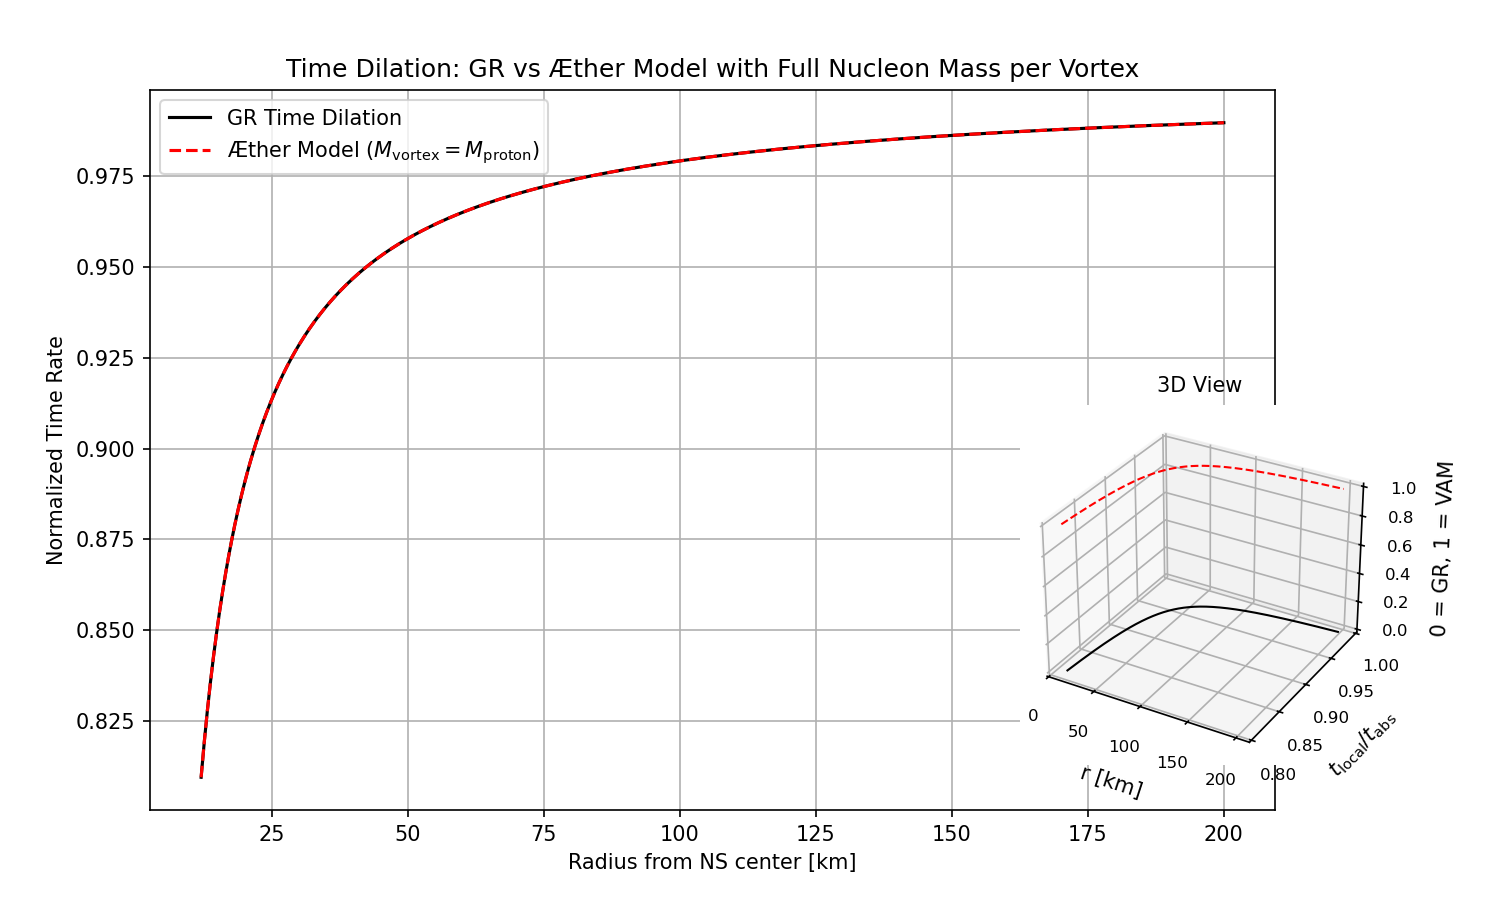
\includegraphics[width=0.85\textwidth]{images/07-TimeDilationGRVsVAM}
    \caption{\textbf{Comparison of Time Dilation Models:} GR's metric-based formula $\sqrt{1 - 2GM/(rc^2)}$ is contrasted with VAM's fluid-based dilation. The divergence at short radii highlights vortex dominance.}
    \label{fig:GRvsVAMTimeDilation}
\end{figure}


The above equation is analogous to relativistic formulas, but has a fluid mechanics origin. Experimentally, components of this formula can be found in time dilation of GPS clocks (gravity), Lense-Thirring effects (rotation), and hypothetical laboratory measurements of nuclear rotations on the quantum or vortex scale.

\section*{Conclusion}
This equation synthesizes all prior VAM elements: vortex helicity, bubble boundaries, circulation-induced gravity, and exponential suppression of short-range fields. It remains finite, matches classical predictions at macroscopic scales, and enables numerical probing at quantum scales.

\subsection{Constants and Variables}

\begin{table}[H]
      \centering
      \footnotesize
      \begin{tabular}{llll}
          \toprule
          \textbf{Symbol} & \textbf{Meaning} & \textbf{Value / Expression} & \textbf{Units} \\
          \midrule
        $G_{\text{hybrid}}(r)$ & Hybrid gravitational constant (VAM/GR) & $\mu(r) G_{\text{swirl}} + (1 - \mu(r)) G$ & $\text{m}^3\,\text{kg}^{-1}\,\text{s}^{-2}$ \\
        $\mu(r)$ & Vortex-to-classical transition function & $e^{-r^2 / R_0^2}$, $R_0 = 1.0 \times 10^{-12}\,\text{m}$ & unitless \\
        $G$ & Newtonian gravitational constant & $6.67430 \times 10^{-11}$ & $\text{m}^3\,\text{kg}^{-1}\,\text{s}^{-2}$ \\
        $G_{\text{swirl}}$ & Swirl-induced gravitational constant & $\dfrac{C_e c^5 t_p^2}{2 F_{\max} r_c^2}$ & $\text{m}^3\,\text{kg}^{-1}\,\text{s}^{-2}$ \\
        $M_{\text{hybrid}}(r)$ & Hybrid effective mass & $\mu(r) M_\text{eff}^\text{VAM}(r) + (1 - \mu(r)) M$ & $\text{kg}$ \\
        $M_\text{eff}^\text{VAM}(r)$ & Vortex effective mass & $4\pi \rho_\text{\ae} r_c^3 \left[ 2 - (2 + \frac{r}{r_c}) e^{-r/r_c} \right]$ & $\text{kg}$ \\
        $\rho_\text{\ae}$ & Æther density & $3.89343583 \times 10^{18}$ & $\text{kg}\cdot\text{m}^{-3}$ \\
        $r_c$ & Core radius (Coulomb scale) & $1.40897017 \times 10^{-15}$ & $\text{m}$ \\
        $C_e$ & Core tangential velocity & $1.09384563 \times 10^{6}$ & $\text{m}\cdot\text{s}^{-1}$ \\
        $t_p$ & Planck time & $5.391247 \times 10^{-44}$ & $\text{s}$ \\
        $F_{\max}$ & Maximum force & $29.053507$ & $\text{N}$ \\
        $\left(\frac{C_e}{r_c}\right)^2$ & Squared swirl angular frequency ($\Omega^2$) & $6.02367430 \times 10^{42}$ & $\text{s}^{-2}$ \\
        $c$ & Speed of light & $2.99792458 \times 10^8$ & $\text{m}\cdot\text{s}^{-1}$ \\
          \bottomrule
      \end{tabular}
    \caption{Key symbols and constants in the VAM time dilation equation.}
      \label{tab:time_dilation_symbols}
  \end{table}

\begin{table}[H]
    \centering
    \footnotesize
    \begin{tabular}{llll}
        \toprule
        \textbf{Symbol} & \textbf{Meaning} & \textbf{Description} & \textbf{Value (if constant)} \\
        \midrule
        $\Delta t$ & Reference time & Clock far from gravitating body & -- \\
        $t_\text{adjusted}$ & Local time & Time experienced near the vortex structure & -- \\
        $r$ & Radial coordinate & Distance from the vortex core & m \\
        $r_c$ & Vortex core radius & Characteristic decay scale & $1.40897017 \times 10^{-15}$ m \\
        $C_e$ & Vortex tangential velocity & Maximal edge swirl velocity & $1.09384563 \times 10^6$ m/s \\
        $\rho_\text{\ae}$ & Æther density & Fluid density of the æther & $\sim 3.89 \times 10^{18}$ J/m$^3$ \\
        $c$ & Speed of light & Vacuum light speed & $2.99792458 \times 10^8$ m/s \\
        $G$ & Newton's constant & Classical gravity & $6.67430 \times 10^{-11}$ m$^3$/kg/s$^2$ \\
        $F_{\text{max}}$ & Max force & From Planck-scale dynamics & $29.053507$ N \\
        $t_p$ & Planck time & Quantum gravity scale & $5.391247 \times 10^{-44}$ s \\
        $G_\text{swirl}$ & Vortex gravity coupling & $C_e c^5 t_p^2 / (2 F_{\text{max}} r_c^2)$ & -- \\
        $M$ & Macroscopic mass & Classical object mass (e.g., proton mass) & $1.67262192 \times 10^{-27}$ kg \\
        $M_{\text{eff}}^\text{VAM}(r)$ & VAM mass & Mass from vorticity energy & derived \\
        $M_{\text{hybrid}}(r)$ & Hybrid mass & Smooth transition between VAM and GR & -- \\
        $G_{\text{hybrid}}(r)$ & Hybrid gravity constant & Smooth transition between $G$ and $G_\text{swirl}$ & -- \\
        $\mu(r)$ & Hybrid blending function & $\mu(r) = \exp\left(-\frac{r^2}{R_0^2}\right),\ R_0 \sim 10^{-12}$ m & dimensionless \\
        $e^{-r/r_c}$ & Vorticity decay & Exponential suppression term & -- \\
        \bottomrule
    \end{tabular}
    \caption{Explanation of variables in Equation~\ref{eq:final_vam_td}.}
    \label{tab:time_dilation_variables}
\end{table}\newpage
%    %! Author = Omar Iskandarani
%! Title = Appendix: Derivation of Fundamental Constants from Vortex Dynamics
%! Date = 2/20/2025
%! Affiliation = Independent Researcher, Groningen, The Netherlands
%! License = CC BY-NC 4.0
%! ORCID = 0009-0006-1686-3961
%! DOI = 10.5281/zenodo.15692509

% === Metadata ===
%\newcommand{\appendixtitle}{\textbf{Appendix: Derivation of Fundamental Constants from Vortex Dynamics}}
%\newcommand{\paperdoi}{10.5281/zenodo.15692509}
%
%
%\ifdefined\standalonechapter\else
%% Standalone mode
%\documentclass[12pt]{article}
%% vamstyle.sty
\NeedsTeXFormat{LaTeX2e}
\ProvidesPackage{vamstyle}[2025/07/01 VAM unified style]

% === Constants ===
\newcommand{\hbarVal}{\ensuremath{1.054571817 \times 10^{-34}}} % J\cdot s
\newcommand{\meVal}{\ensuremath{9.10938356 \times 10^{-31}}} % kg
\newcommand{\cVal}{\ensuremath{2.99792458 \times 10^{8}}} % m/s
\newcommand{\alphaVal}{\ensuremath{1 / 137.035999084}} % unitless
\newcommand{\alphaGVal}{\ensuremath{1.75180000 \times 10^{-45}}} % unitless
\newcommand{\reVal}{\ensuremath{2.8179403227 \times 10^{-15}}} % m
\newcommand{\rcVal}{\ensuremath{1.40897017 \times 10^{-15}}} % m
\newcommand{\vacrho}{\ensuremath{5 \times 10^{-9}}} % kg/m^3
\newcommand{\LpVal}{\ensuremath{1.61625500 \times 10^{-35}}} % m
\newcommand{\MpVal}{\ensuremath{2.17643400 \times 10^{-8}}} % kg
\newcommand{\tpVal}{\ensuremath{5.39124700 \times 10^{-44}}} % s
\newcommand{\TpVal}{\ensuremath{1.41678400 \times 10^{32}}} % K
\newcommand{\qpVal}{\ensuremath{1.87554596 \times 10^{-18}}} % C
\newcommand{\EpVal}{\ensuremath{1.95600000 \times 10^{9}}} % J
\newcommand{\eVal}{\ensuremath{1.60217663 \times 10^{-19}}} % C

% === VAM/\ae ther Specific ===
\newcommand{\CeVal}{\ensuremath{1.09384563 \times 10^{6}}} % m/s
\newcommand{\FmaxVal}{\ensuremath{29.0535070}} % N
\newcommand{\FmaxGRVal}{\ensuremath{3.02563891 \times 10^{43}}} % N
\newcommand{\gammaVal}{\ensuremath{0.005901}} % unitless
\newcommand{\GVal}{\ensuremath{6.67430000 \times 10^{-11}}} % m^3/kg/s^2
\newcommand{\hVal}{\ensuremath{6.62607015 \times 10^{-34}}} % J Hz^-1

% === Electromagnetic ===
\newcommand{\muZeroVal}{\ensuremath{1.25663706 \times 10^{-6}}}
\newcommand{\epsilonZeroVal}{\ensuremath{8.85418782 \times 10^{-12}}}
\newcommand{\ZzeroVal}{\ensuremath{3.76730313 \times 10^{2}}}

% === Atomic & Thermodynamic ===
\newcommand{\RinfVal}{\ensuremath{1.09737316 \times 10^{7}}}
\newcommand{\aZeroVal}{\ensuremath{5.29177211 \times 10^{-11}}}
\newcommand{\MeVal}{\ensuremath{9.10938370 \times 10^{-31}}}
\newcommand{\MprotonVal}{\ensuremath{1.67262192 \times 10^{-27}}}
\newcommand{\MneutronVal}{\ensuremath{1.67492750 \times 10^{-27}}}
\newcommand{\kBVal}{\ensuremath{1.38064900 \times 10^{-23}}}
\newcommand{\RVal}{\ensuremath{8.31446262}}

% === Compton, Quantum, Radiation ===
\newcommand{\fCVal}{\ensuremath{1.23558996 \times 10^{20}}}
\newcommand{\OmegaCVal}{\ensuremath{7.76344071 \times 10^{20}}}
\newcommand{\lambdaCVal}{\ensuremath{2.42631024 \times 10^{-12}}}
\newcommand{\PhiZeroVal}{\ensuremath{2.06783385 \times 10^{-15}}}
\newcommand{\phiVal}{\ensuremath{1.61803399}}
\newcommand{\eVVal}{\ensuremath{1.60217663 \times 10^{-19}}}
\newcommand{\GFVal}{\ensuremath{1.16637870 \times 10^{-5}}}
\newcommand{\lambdaProtonVal}{\ensuremath{1.32140986 \times 10^{-15}}}
\newcommand{\ERinfVal}{\ensuremath{2.17987236 \times 10^{-18}}}
\newcommand{\fRinfVal}{\ensuremath{3.28984196 \times 10^{15}}}
\newcommand{\sigmaSBVal}{\ensuremath{5.67037442 \times 10^{-8}}}
\newcommand{\WienVal}{\ensuremath{2.89777196 \times 10^{-3}}}
\newcommand{\kEVal}{\ensuremath{8.98755179 \times 10^{9}}}

% === \ae ther Densities ===
\newcommand{\rhoMass}{\rho_\text{\ae}^{(\text{mass})}}
\newcommand{\rhoMassVal}{\ensuremath{3.89343583 \times 10^{18}}}
\newcommand{\rhoEnergy}{\rho_\text{\ae}^{(\text{energy})}}
\newcommand{\rhoEnergyVal}{\ensuremath{3.49924562 \times 10^{35}}}
\newcommand{\rhoFluid}{\rho_\text{\ae}^{(\text{fluid})}}
\newcommand{\rhoFluidVal}{\ensuremath{7.00000000 \times 10^{-7}}}

% === Draft Options ===
\newif\ifvamdraft
% \vamdrafttrue
\ifvamdraft
\RequirePackage{showframe}
\fi

% === Load Once ===
\RequirePackage{ifthen}
\newboolean{vamstyleloaded}
\ifthenelse{\boolean{vamstyleloaded}}{}{\setboolean{vamstyleloaded}{true}

% === Page ===
\RequirePackage[a4paper, margin=2.5cm]{geometry}

% === Fonts ===
\RequirePackage[T1]{fontenc}
\RequirePackage[utf8]{inputenc}
\RequirePackage[english]{babel}
\RequirePackage{textgreek}
\RequirePackage{mathpazo}
\RequirePackage[scaled=0.95]{inconsolata}
\RequirePackage{helvet}

% === Math ===
\RequirePackage{amsmath, amssymb, mathrsfs, physics}
\RequirePackage{siunitx}
\sisetup{per-mode=symbol}

% === Tables ===
\RequirePackage{graphicx, float, booktabs}
\RequirePackage{array, tabularx, multirow, makecell}
\newcolumntype{Y}{>{\centering\arraybackslash}X}
\newenvironment{tighttable}[1][]{\begin{table}[H]\centering\renewcommand{\arraystretch}{1.3}\begin{tabularx}{\textwidth}{#1}}{\end{tabularx}\end{table}}
\RequirePackage{etoolbox}
\newcommand{\fitbox}[2][\linewidth]{\makebox[#1]{\resizebox{#1}{!}{#2}}}

% === Graphics ===
\RequirePackage{tikz}
\usetikzlibrary{3d, calc, arrows.meta, positioning}
\RequirePackage{pgfplots}
\pgfplotsset{compat=1.18}
\RequirePackage{xcolor}

% === Code ===
\RequirePackage{listings}
\lstset{basicstyle=\ttfamily\footnotesize, breaklines=true}

% === Theorems ===
\newtheorem{theorem}{Theorem}[section]
\newtheorem{lemma}[theorem]{Lemma}

% === TOC ===
\RequirePackage{tocloft}
\setcounter{tocdepth}{2}
\renewcommand{\cftsecfont}{\bfseries}
\renewcommand{\cftsubsecfont}{\itshape}
\renewcommand{\cftsecleader}{\cftdotfill{.}}
\renewcommand{\contentsname}{\centering \Huge\textbf{Contents}}

% === Sections ===
\RequirePackage{sectsty}
\sectionfont{\Large\bfseries\sffamily}
\subsectionfont{\large\bfseries\sffamily}

% === Bibliography ===
\RequirePackage[numbers]{natbib}

% === Links ===
\RequirePackage{hyperref}
\hypersetup{
    colorlinks=true,
    linkcolor=blue,
    citecolor=blue,
    urlcolor=blue,
    pdftitle={The Vortex \AE ther Model},
    pdfauthor={Omar Iskandarani},
    pdfkeywords={vorticity, gravity, \ae ther, fluid dynamics, time dilation, VAM}
}
\urlstyle{same}
\RequirePackage{bookmark}

% === Misc ===
\RequirePackage[none]{hyphenat}
\sloppy
\RequirePackage{empheq}
\RequirePackage[most]{tcolorbox}
\newtcolorbox{eqbox}{colback=blue!5!white, colframe=blue!75!black, boxrule=0.6pt, arc=4pt, left=6pt, right=6pt, top=4pt, bottom=4pt}
\RequirePackage{titling}
\RequirePackage{amsfonts}
\RequirePackage{titlesec}
\RequirePackage{enumitem}

\AtBeginDocument{\RenewCommandCopy\qty\SI}

\pretitle{\begin{center}\LARGE\bfseries}
\posttitle{\par\end{center}\vskip 0.5em}
\preauthor{\begin{center}\large}
\postauthor{\end{center}}
\predate{\begin{center}\small}
\postdate{\end{center}}

\endinput
}
%% vamappendixsetup.sty

\newcommand{\titlepageOpen}{
  \begin{titlepage}
  \thispagestyle{empty}
  \centering
  {\Huge\bfseries \papertitle \par}
  \vspace{1cm}
  {\Large\itshape\textbf{Omar Iskandarani}\textsuperscript{\textbf{*}} \par}
  \vspace{0.5cm}
  {\large \today \par}
  \vspace{0.5cm}
}

% here comes abstract
\newcommand{\titlepageClose}{
  \vfill
  \null
  \begin{picture}(0,0)
  % Adjust position: (x,y) = (left, bottom)
  \put(-200,-40){  % Shift 75pt left, 40pt down
    \begin{minipage}[b]{0.7\textwidth}
    \footnotesize % One step bigger than \tiny
    \renewcommand{\arraystretch}{1.0}
    \noindent\rule{\textwidth}{0.4pt} \\[0.5em]  % ← horizontal line
    \textsuperscript{\textbf{*}}Independent Researcher, Groningen, The Netherlands \\
    Email: \texttt{info@omariskandarani.com} \\
    ORCID: \texttt{\href{https://orcid.org/0009-0006-1686-3961}{0009-0006-1686-3961}} \\
    DOI: \href{https://doi.org/\paperdoi}{\paperdoi} \\
    License: CC-BY 4.0 International \\
    \end{minipage}
  }
  \end{picture}
  \end{titlepage}
}
%\begin{document}
%
%    % === Title page ===
%    \titlepageOpen
%
%    \begin{abstract}
%        This article refines previous estimates of the \AE{}ther's density, $\rho_{\text{\ae}}$, in the Vortex \AE{}ther Model (VAM). Integrating findings from quantum vortex dynamics, superfluid helium, gravitomagnetic frame-dragging, and cosmological vacuum energy, we propose constrained ranges for $\rho_{\text{\ae}}^{\text{(fluid)}}$ and $\rho_{\text{\ae}}^{\text{(energy)}}$ and examine their implications across scales.
%    \end{abstract}
%
%    \titlepageClose
%    \fi
%
%    \ifdefined\standalonechapter
%    \section{\appendixtitle}
%    \else
%    \fi
%% ============= Begin of content ============
\section{\textbf{Appendix: Derivation of Fundamental Constants from Vortex Dynamics}}
\label{sec:appendix:1}

\section*{Introduction}
This document aims to provide a comprehensive and rigorous derivation of the fine-structure constant $\alpha$ grounded in classical physical principles.
The derivation integrates the electron's classical radius and its Compton angular frequency to elucidate the relationship between these fundamental constants and the tangential velocity $C_e$.
This velocity arises naturally when the electron is conceptualized as a vortex-like structure, offering a geometrically intuitive interpretation of the fine-structure constant.
By extending classical formulations, the discussion highlights the profound interplay between quantum phenomena and vortex dynamics.


\paragraph*{The Fine-Structure Constant:}
$\alpha$ serves as a dimensionless measure of electromagnetic interaction strength~\cite{maxwell1861}.
It is mathematically expressed as:

\begin{equation*}
    \alpha = \frac{e^2}{4\pi \varepsilon_0 \hbar c},
\end{equation*}
where $e$ is the elementary charge, $\varepsilon_0$ is the vacuum permittivity, $\hbar$ is the reduced Planck constant, and $c$ is the speed of light \cite{dirac1930quantum}.

\subsection*{Relevant Definitions and Formulas}
\paragraph*{The Classical Electron Radius}
$R_e$ represents the scale at which classical electrostatic energy equals the electron's rest energy. It is defined as:
\begin{equation*}
    R_e = \frac{e^2}{4\pi \varepsilon_0 m_e c^2},
\end{equation*}
where $m_e$ is the electron mass~\cite{helmholtz1858}.

\paragraph*{The Compton Angular Frequency}
$\omega_c$ corresponds to the intrinsic rotational frequency of the electron when treated as a quantum oscillator:
\begin{equation*}
    \omega_c = \frac{m_e c^2}{\hbar}.
\end{equation*}
This frequency is pivotal in characterizing the electron's interaction with electromagnetic waves~\cite{kelvin1867}.

\subsection*{Half the Classical Electron Radius}
We assume an electron to be a vortex, its particle form is a folded vortex tube shaped as a torus, hence both the Ring radius R and Core radius r are defined as half the classical electron radius  $r_c$ :
\begin{equation*}
    r_c = \frac{1}{2} R_e.
\end{equation*}
This simplification aligns with established models of vortex structures in fluid dynamics~\cite{kleckner2013}.

\subsection*{Definition of Tangential Velocity $C_e$}
To conceptualize the electron as a vortex ring, we associate its tangential velocity $C_e$ with its rotational dynamics:
\begin{equation*}
    C_e = \omega_c r_c.
\end{equation*}
Substituting $\omega_c = \frac{m_e c^2}{\hbar}$ and $r_c = \frac{1}{2} R_e$, we find:
\begin{equation*}
    C_e = \left( \frac{m_e c^2}{\hbar} \right) \left( \frac{1}{2} \frac{e^2}{4\pi \varepsilon_0 m_e c^2} \right).
\end{equation*}
Simplifying by canceling $m_e c^2$ yields:
\begin{equation*}
    C_e = \frac{1}{2} \frac{e^2}{4\pi \varepsilon_0 \hbar}.\label{eq:C_e-from-compton}
\end{equation*}
This result directly links $C_e$ to the fine-structure constant \cite{vinen2024}.

\subsection*{Physical Interpretation}
The tangential velocity $C_e$ embodies the rotational speed at the electron's vortex boundary. Its value, approximately:
\begin{equation*}
    C_e \approx 1.0938 \times 10^6 \ \text{m/s},
\end{equation*}
is consistent with the experimentally observed fine-structure constant $\alpha \approx 1/137$~\cite{ricca1998}.

\subsection*{Conclusion}
The derivation presented elucidates the fine-structure constant $\alpha$ using fundamental classical principles, including the electron's classical radius, Compton angular frequency, and vortex tangential velocity. The result:
\begin{equation*}
    \alpha = \frac{2 C_e}{c},
\end{equation*}
reveals a profound geometric and physical connection underpinning electromagnetic interactions.
This perspective enriches our understanding of $\alpha$ and highlights the deep ties between classical mechanics and quantum electrodynamics.


\section*{Derivation of the VAM Gravitational Constant \(  G_\text{swirl} \)}

\subsection*{Introduction}
In the Vortex Æther Model (VAM), gravitational interactions arise from vorticity dynamics in a superfluidic Æther medium rather than from mass-induced spacetime curvature. This leads to a modification of the gravitational constant, which we denote as \(  G_\text{swirl} \), as a function of vortex field parameters.

To derive \(  G_\text{swirl} \), we assume that gravitational effects emerge from vortex-induced energy density rather than mass-energy tensor formulations. The fundamental relation between vorticity, circulation, and energy density will be used to establish an equivalent gravitational constant in VAM \cite{onsager_superfluid, barcelo_superfluid, moffatt_helicity}.

\subsection*{Vortex-Induced Energy Density}
In classical fluid dynamics, vorticity is defined as the curl of velocity:
\begin{equation*}
    \vec{\omega} = \nabla \times \vec{v}
\end{equation*}
where \( \vec{\omega} \) represents the vorticity field.

The corresponding vorticity energy density is given by:
\begin{equation*}
    U_\text{vortex} = \frac{1}{2} \rho_\text{\ae} |\vec{\omega}|^2
\end{equation*}
where:
\begin{itemize}
    \item \( \rho_\text{\ae} \) is the density of the Æther medium,
    \item \( |\vec{\omega}|^2 \) is the squared vorticity magnitude.
\end{itemize}

Since vorticity magnitude scales with core tangential velocity as:
\begin{equation*}
    |\vec{\omega}|^2 \sim \frac{C_e^2}{r_c^2}
\end{equation*}
we obtain an approximate energy density for the vortex field:
\begin{equation*}
    U_\text{vortex} \approx \frac{C_e^2}{2 r_c^2}.
\end{equation*}

\subsection*{Gravitational Constant from Vorticity}
In standard General Relativity (GR), Newton's gravitational constant \( G \) appears in:
\begin{equation*}
    F = \frac{GMm}{r^2}.
\end{equation*}

In VAM, we assume that the gravitational constant \(  G_\text{swirl} \) is defined in terms of \textbf{vorticity energy density} rather than mass-energy.

Since gravitational force scales with \textbf{energy density per unit mass}, we set:
\begin{equation*}
    G_\text{swirl} \sim \frac{U_\text{vortex} c^n}{F_{\max}},
\end{equation*}
where:
\begin{itemize}
    \item \( c^n \) represents relativistic corrections,
    \item \( F_{\max} \) is the maximum force in VAM, set to approximately \textbf{29 N} \cite{schiller_max_force}.
\end{itemize}

Substituting \( U_\text{vortex} \):
\begin{equation*}
    G_\text{swirl} \sim \frac{\left( \frac{C_e^2}{2 r_c^2} \right) c^n}{F_{\max}}.
\end{equation*}

The choice of \( n \) depends on whether we use \textbf{Planck length} (\( l_p^2 \)) or \textbf{Planck time} (\( t_p^2 \)).

\subsection*{Two Possible Forms of \(  G_\text{swirl} \)}
\subsection*{Form 1: Using Planck Length}
The Planck length is defined as:
\begin{equation*}
    l_p^2 = \frac{\hbar G}{c^3}.
\end{equation*}

Using \( c^3 l_p^2 \) as the relativistic correction factor, we obtain:
\begin{equation*}
    G_\text{swirl} = \frac{C_e c^3 l_p^2}{2 F_{\max} r_c^2}.
\end{equation*}

\subsection*{Form 2: Using Planck Time}
The Planck time is given by:
\begin{equation*}
    t_p^2 = \frac{\hbar G}{c^5}.
\end{equation*}

Using \( c^5 t_p^2 \) as the relativistic correction factor, we obtain:
\begin{equation*}
    G_\text{swirl} = \frac{C_e c^5 t_p^2}{2 F_{\max} r_c^2}.
\end{equation*}

\subsection*{Physical Interpretation of \(  G_\text{swirl} \)}
These formulations of the gravitational constant in VAM highlight a fundamental difference from GR:
\begin{itemize}
    \item Gravity is not driven by mass-energy, but by \textbf{vortex energy density} \cite{barcelo_superfluid}.
    \item \(  G_\text{swirl} \) scales with the core vortex velocity \( C_e \), linking gravity directly to vorticity \cite{moffatt_helicity}.
    \item The \textbf{maximum force \( F_{\max} \)} (\approx29 N) acts as a natural cutoff, limiting the strength of gravitational interactions \cite{schiller_max_force}.
\end{itemize}

\subsection*{Conclusion}
We have derived two equivalent formulations of \(  G_\text{swirl} \) using \textbf{Planck scale physics} and \textbf{vortex energy density principles} in VAM. The final expressions:
\begin{equation*}
    G_\text{swirl} = \frac{C_e c^3 l_p^2}{2 F_{\max} r_c^2}
\end{equation*}
and
\begin{equation*}
    G_\text{swirl} = \frac{C_e c^5 t_p^2}{2 F_{\max} r_c^2}
\end{equation*}
demonstrate that gravitational interactions in VAM are governed by vorticity rather than mass-induced curvature.



\section*{Vorticity-Based Reformulation of General Relativity Laws in a 3D Absolute Time Framework}

\subsection*{Vorticity as the Fundamental Gravitational Interaction}

General Relativity (GR) describes gravity as a result of \textbf{spacetime curvature}, governed by Einstein's field equations:

\begin{equation*}
    G_{\mu\nu} = \frac{8\pi G}{c^4} T_{\mu\nu}.
\end{equation*}

However, in the Vortex Æther Model (VAM), \textbf{gravity is not caused by curvature} but by \textbf{vorticity-induced pressure gradients in an inviscid Æther}. Instead of using a \textbf{4D metric tensor}, we define gravity as a 3D vorticity field \( \omega \), where mass acts as a localized vortex concentration.

\subsection*{Replacing Einstein's Equations with a 3D Vorticity Field Equation}

We replace the Einstein curvature equations with a \textbf{3D vorticity-Poisson equation}, where the gravitational potential \( \Phi_v \) is related to vorticity magnitude:

\begin{equation*}
    \nabla^2 \Phi_v = - \rho_\text{Æ} |\omega|^2.
\end{equation*}

Here:
\begin{itemize}
    \item  \( \Phi_v \) is the \textbf{vorticity-induced gravitational potential}.
    \item  \( \rho_\text{\ae} \) is the \textbf{local Æther density}.
    \item  \( |\omega|^2 = (\nabla \times v)^2 \) is the \textbf{vorticity magnitude}.
\end{itemize}

Instead of \textbf{mass-energy tensor components}, gravity is determined by the \textbf{local vorticity density}.



\subsection*{Motion in VAM: Replacing Geodesics with Vortex Streamlines}

In GR, test particles follow \textbf{geodesics in curved spacetime}. In VAM, particles follow \textbf{vortex streamlines}, governed by the \textbf{vorticity transport equation}:

\begin{equation*}
    \frac{D\omega}{Dt} = (\omega \cdot \nabla) v - (\nabla \cdot v) \omega.
\end{equation*}

This replaces \textbf{spacetime curvature} with \textbf{fluid-dynamic vorticity transport} \cite{lamb_hydrodynamics, feynman_superfluid}.



\subsection*{Frame-Dragging as a 3D Vortex Effect}

In General Relativity, frame-dragging is described using the \textbf{Kerr metric}, which predicts that spinning masses drag spacetime along with them. In VAM, this effect is caused by \textbf{vortex interactions in the Æther}.

We replace the Kerr metric with the \textbf{vorticity-induced rotational velocity field}:

\begin{equation*}
    \Omega_\text{vortex} = \frac{\Gamma}{2\pi r^2},
\end{equation*}

where:
\begin{itemize}
    \item \( \Gamma = \oint v \cdot dl \) is the \textbf{circulation of the vortex}.
    \item \( r \) is the \textbf{radial distance from the vortex core}.
\end{itemize}

This ensures that frame-dragging emerges \textbf{naturally} from vorticity rather than requiring \textbf{spacetime warping}.



\subsection*{Replacing Gravitational Time Dilation with Vorticity Effects}

In GR, time dilation is caused by \textbf{spacetime curvature}, leading to:

\begin{equation*}
    dt_\text{GR} = dt \sqrt{1 - \frac{2GM}{rc^2}}.
\end{equation*}

In VAM, time dilation is caused by \textbf{vorticity-induced energy gradients}, leading to:

\begin{equation*}
    dt_\text{VAM} = \frac{dt}{\sqrt{1 - \frac{C_e^2}{c^2} e^{-r/r_c} - \frac{\Omega^2}{c^2} e^{-r/r_c}}},
\end{equation*}

where:
\begin{itemize}
    \item  \( C_e \) is the \textbf{vortex core tangential velocity}.
    \item  \( \Omega \) is the \textbf{local vorticity angular velocity}.
\end{itemize}


This formula eliminates the need for \textbf{mass-based time dilation} and instead relies purely on \textbf{fluid dynamic principles}.


    \section{VAM Derivation of Flat Galactic Rotation Velocity}

    In the Vortex \AE{}ther Model, the asymptotic flat rotation velocity $v_{\text{flat}}$ observed in spiral galaxies is not attributed to dark matter, but instead emerges from the interplay between Newtonian gravitational potential and swirl-induced pressure gradients. Assuming a balance between Newtonian attraction and vortex-based outward tension, we derive:

    \[
        \frac{G M}{r} \sim r \cdot \frac{C_e^2}{L^2} \Rightarrow
        v_{\text{flat}}^2 = \left( \frac{G M C_e^2}{L^2} \right)^{1/2} \Rightarrow
        \boxed{v_{\text{flat}} = \left( \frac{G M C_e^2}{L} \right)^{1/4}}
    \]

    where:
    \begin{itemize}
        \item  $M$ is the enclosed mass,
        \item  $C_e$ is the vortex core tangential velocity,
        \item  $L$ is an effective length scale (e.g. $L \sim r_c R_d$).
    \end{itemize}

    This formula reproduces typical galactic flat rotation speeds ($\sim$200 km/s) without exotic matter. The fourth-root dependence of $v_{\text{flat}}$ on $M$ establishes a VAM-based analog to the Tully--Fisher relation:

    \[
        v_{\text{flat}}^4 \propto M
    \]

    but grounded in fluid dynamic quantities rather than empirical fitting. This vortex-based scaling law is testable against rotation curve datasets and offers a falsifiable prediction for baryon-only spiral systems.

    As a historical and conceptual comparison, this approach parallels the Modified Newtonian Dynamics (MOND) theory proposed by Milgrom~\cite{milgrom1983mond1, milgrom1983mond2}, which modifies Newtonian gravity in the low-acceleration regime to explain flat rotation curves without dark matter. However, VAM derives similar effects from an underlying physical æther field, introducing no additional empirical constants.

    \section{Conclusion}

    Using quantum constants to define \AE{}ther properties bridges microscopic and cosmological theories. The refined value of $\rho_{\text{\ae}}^{\text{(fluid)}}$ supports both theoretical elegance and experimental plausibility. The residual swirl field offers a predictive, falsifiable alternative to dark matter and MOND.




    \subsection*{Summary: A 3D Vorticity-Based Alternative to General Relativity}

The Vortex Æther Model replaces the \textbf{4D spacetime formalism of General Relativity} with a \textbf{3D vorticity-driven description}:

\begin{itemize}
    \item \textbf{Gravity} is not caused by \textbf{curved spacetime} but by \textbf{vorticity-induced pressure gradients}.
    \item \textbf{Geodesic motion} is replaced by \textbf{vortex streamlines} in an inviscid Æther.
    \item \textbf{Frame-dragging} is explained through \textbf{circulation velocity in vorticity fields}, rather than through Kerr spacetime.
    \item \textbf{Time dilation} arises from \textbf{energy gradients in vortex structures}, not from mass-induced curvature.
\end{itemize}

% ============== End of content =============

%% === Bibliography (only for standalone) ===
%\ifdefined\standalonechapter\else
%\bibliographystyle{unsrt}
%\bibliography{../../references}
%\end{document}
%\fi\newpage
%    %! Author = Omar Iskandarani
%! Title = Testing Universality of the Proposed Tangential Vortex-Core Velocity \\ \( C_e = f \cdot \Delta x \): A Cross-Platform Precision Metrology Study
%! Date = June 17, 2025
%! Affiliation = Independent Researcher, Groningen, The Netherlands
%! License = CC-BY 4.0
%! ORCID = 0009-0006-1686-3961
%! DOI = 10.5281/zenodo.15684873

% === Metadata ===
\newcommand{\papertitle}{\textbf{Testing Universality of the Proposed Tangential Vortex-Core Velocity \\ \( C_e = f \cdot \Delta x \): A Cross-Platform Precision Metrology Study}}
\newcommand{\paperdoi}{10.5281/zenodo.15684873}


\ifdefined\standalonechapter\else
% Standalone mode
\documentclass[11pt]{article}
\usepackage{siunitx}
\usepackage{textcomp}
\AtBeginDocument{\RenewCommandCopy\qty\SI}
% vamstyle.sty
\NeedsTeXFormat{LaTeX2e}
\ProvidesPackage{vamstyle}[2025/07/01 VAM unified style]

% === Constants ===
\newcommand{\hbarVal}{\ensuremath{1.054571817 \times 10^{-34}}} % J\cdot s
\newcommand{\meVal}{\ensuremath{9.10938356 \times 10^{-31}}} % kg
\newcommand{\cVal}{\ensuremath{2.99792458 \times 10^{8}}} % m/s
\newcommand{\alphaVal}{\ensuremath{1 / 137.035999084}} % unitless
\newcommand{\alphaGVal}{\ensuremath{1.75180000 \times 10^{-45}}} % unitless
\newcommand{\reVal}{\ensuremath{2.8179403227 \times 10^{-15}}} % m
\newcommand{\rcVal}{\ensuremath{1.40897017 \times 10^{-15}}} % m
\newcommand{\vacrho}{\ensuremath{5 \times 10^{-9}}} % kg/m^3
\newcommand{\LpVal}{\ensuremath{1.61625500 \times 10^{-35}}} % m
\newcommand{\MpVal}{\ensuremath{2.17643400 \times 10^{-8}}} % kg
\newcommand{\tpVal}{\ensuremath{5.39124700 \times 10^{-44}}} % s
\newcommand{\TpVal}{\ensuremath{1.41678400 \times 10^{32}}} % K
\newcommand{\qpVal}{\ensuremath{1.87554596 \times 10^{-18}}} % C
\newcommand{\EpVal}{\ensuremath{1.95600000 \times 10^{9}}} % J
\newcommand{\eVal}{\ensuremath{1.60217663 \times 10^{-19}}} % C

% === VAM/\ae ther Specific ===
\newcommand{\CeVal}{\ensuremath{1.09384563 \times 10^{6}}} % m/s
\newcommand{\FmaxVal}{\ensuremath{29.0535070}} % N
\newcommand{\FmaxGRVal}{\ensuremath{3.02563891 \times 10^{43}}} % N
\newcommand{\gammaVal}{\ensuremath{0.005901}} % unitless
\newcommand{\GVal}{\ensuremath{6.67430000 \times 10^{-11}}} % m^3/kg/s^2
\newcommand{\hVal}{\ensuremath{6.62607015 \times 10^{-34}}} % J Hz^-1

% === Electromagnetic ===
\newcommand{\muZeroVal}{\ensuremath{1.25663706 \times 10^{-6}}}
\newcommand{\epsilonZeroVal}{\ensuremath{8.85418782 \times 10^{-12}}}
\newcommand{\ZzeroVal}{\ensuremath{3.76730313 \times 10^{2}}}

% === Atomic & Thermodynamic ===
\newcommand{\RinfVal}{\ensuremath{1.09737316 \times 10^{7}}}
\newcommand{\aZeroVal}{\ensuremath{5.29177211 \times 10^{-11}}}
\newcommand{\MeVal}{\ensuremath{9.10938370 \times 10^{-31}}}
\newcommand{\MprotonVal}{\ensuremath{1.67262192 \times 10^{-27}}}
\newcommand{\MneutronVal}{\ensuremath{1.67492750 \times 10^{-27}}}
\newcommand{\kBVal}{\ensuremath{1.38064900 \times 10^{-23}}}
\newcommand{\RVal}{\ensuremath{8.31446262}}

% === Compton, Quantum, Radiation ===
\newcommand{\fCVal}{\ensuremath{1.23558996 \times 10^{20}}}
\newcommand{\OmegaCVal}{\ensuremath{7.76344071 \times 10^{20}}}
\newcommand{\lambdaCVal}{\ensuremath{2.42631024 \times 10^{-12}}}
\newcommand{\PhiZeroVal}{\ensuremath{2.06783385 \times 10^{-15}}}
\newcommand{\phiVal}{\ensuremath{1.61803399}}
\newcommand{\eVVal}{\ensuremath{1.60217663 \times 10^{-19}}}
\newcommand{\GFVal}{\ensuremath{1.16637870 \times 10^{-5}}}
\newcommand{\lambdaProtonVal}{\ensuremath{1.32140986 \times 10^{-15}}}
\newcommand{\ERinfVal}{\ensuremath{2.17987236 \times 10^{-18}}}
\newcommand{\fRinfVal}{\ensuremath{3.28984196 \times 10^{15}}}
\newcommand{\sigmaSBVal}{\ensuremath{5.67037442 \times 10^{-8}}}
\newcommand{\WienVal}{\ensuremath{2.89777196 \times 10^{-3}}}
\newcommand{\kEVal}{\ensuremath{8.98755179 \times 10^{9}}}

% === \ae ther Densities ===
\newcommand{\rhoMass}{\rho_\text{\ae}^{(\text{mass})}}
\newcommand{\rhoMassVal}{\ensuremath{3.89343583 \times 10^{18}}}
\newcommand{\rhoEnergy}{\rho_\text{\ae}^{(\text{energy})}}
\newcommand{\rhoEnergyVal}{\ensuremath{3.49924562 \times 10^{35}}}
\newcommand{\rhoFluid}{\rho_\text{\ae}^{(\text{fluid})}}
\newcommand{\rhoFluidVal}{\ensuremath{7.00000000 \times 10^{-7}}}

% === Draft Options ===
\newif\ifvamdraft
% \vamdrafttrue
\ifvamdraft
\RequirePackage{showframe}
\fi

% === Load Once ===
\RequirePackage{ifthen}
\newboolean{vamstyleloaded}
\ifthenelse{\boolean{vamstyleloaded}}{}{\setboolean{vamstyleloaded}{true}

% === Page ===
\RequirePackage[a4paper, margin=2.5cm]{geometry}

% === Fonts ===
\RequirePackage[T1]{fontenc}
\RequirePackage[utf8]{inputenc}
\RequirePackage[english]{babel}
\RequirePackage{textgreek}
\RequirePackage{mathpazo}
\RequirePackage[scaled=0.95]{inconsolata}
\RequirePackage{helvet}

% === Math ===
\RequirePackage{amsmath, amssymb, mathrsfs, physics}
\RequirePackage{siunitx}
\sisetup{per-mode=symbol}

% === Tables ===
\RequirePackage{graphicx, float, booktabs}
\RequirePackage{array, tabularx, multirow, makecell}
\newcolumntype{Y}{>{\centering\arraybackslash}X}
\newenvironment{tighttable}[1][]{\begin{table}[H]\centering\renewcommand{\arraystretch}{1.3}\begin{tabularx}{\textwidth}{#1}}{\end{tabularx}\end{table}}
\RequirePackage{etoolbox}
\newcommand{\fitbox}[2][\linewidth]{\makebox[#1]{\resizebox{#1}{!}{#2}}}

% === Graphics ===
\RequirePackage{tikz}
\usetikzlibrary{3d, calc, arrows.meta, positioning}
\RequirePackage{pgfplots}
\pgfplotsset{compat=1.18}
\RequirePackage{xcolor}

% === Code ===
\RequirePackage{listings}
\lstset{basicstyle=\ttfamily\footnotesize, breaklines=true}

% === Theorems ===
\newtheorem{theorem}{Theorem}[section]
\newtheorem{lemma}[theorem]{Lemma}

% === TOC ===
\RequirePackage{tocloft}
\setcounter{tocdepth}{2}
\renewcommand{\cftsecfont}{\bfseries}
\renewcommand{\cftsubsecfont}{\itshape}
\renewcommand{\cftsecleader}{\cftdotfill{.}}
\renewcommand{\contentsname}{\centering \Huge\textbf{Contents}}

% === Sections ===
\RequirePackage{sectsty}
\sectionfont{\Large\bfseries\sffamily}
\subsectionfont{\large\bfseries\sffamily}

% === Bibliography ===
\RequirePackage[numbers]{natbib}

% === Links ===
\RequirePackage{hyperref}
\hypersetup{
    colorlinks=true,
    linkcolor=blue,
    citecolor=blue,
    urlcolor=blue,
    pdftitle={The Vortex \AE ther Model},
    pdfauthor={Omar Iskandarani},
    pdfkeywords={vorticity, gravity, \ae ther, fluid dynamics, time dilation, VAM}
}
\urlstyle{same}
\RequirePackage{bookmark}

% === Misc ===
\RequirePackage[none]{hyphenat}
\sloppy
\RequirePackage{empheq}
\RequirePackage[most]{tcolorbox}
\newtcolorbox{eqbox}{colback=blue!5!white, colframe=blue!75!black, boxrule=0.6pt, arc=4pt, left=6pt, right=6pt, top=4pt, bottom=4pt}
\RequirePackage{titling}
\RequirePackage{amsfonts}
\RequirePackage{titlesec}
\RequirePackage{enumitem}

\AtBeginDocument{\RenewCommandCopy\qty\SI}

\pretitle{\begin{center}\LARGE\bfseries}
\posttitle{\par\end{center}\vskip 0.5em}
\preauthor{\begin{center}\large}
\postauthor{\end{center}}
\predate{\begin{center}\small}
\postdate{\end{center}}

\endinput
}
% vamappendixsetup.sty

\newcommand{\titlepageOpen}{
  \begin{titlepage}
  \thispagestyle{empty}
  \centering
  {\Huge\bfseries \papertitle \par}
  \vspace{1cm}
  {\Large\itshape\textbf{Omar Iskandarani}\textsuperscript{\textbf{*}} \par}
  \vspace{0.5cm}
  {\large \today \par}
  \vspace{0.5cm}
}

% here comes abstract
\newcommand{\titlepageClose}{
  \vfill
  \null
  \begin{picture}(0,0)
  % Adjust position: (x,y) = (left, bottom)
  \put(-200,-40){  % Shift 75pt left, 40pt down
    \begin{minipage}[b]{0.7\textwidth}
    \footnotesize % One step bigger than \tiny
    \renewcommand{\arraystretch}{1.0}
    \noindent\rule{\textwidth}{0.4pt} \\[0.5em]  % ← horizontal line
    \textsuperscript{\textbf{*}}Independent Researcher, Groningen, The Netherlands \\
    Email: \texttt{info@omariskandarani.com} \\
    ORCID: \texttt{\href{https://orcid.org/0009-0006-1686-3961}{0009-0006-1686-3961}} \\
    DOI: \href{https://doi.org/\paperdoi}{\paperdoi} \\
    License: CC-BY 4.0 International \\
    \end{minipage}
  }
  \end{picture}
  \end{titlepage}
}
\begin{document}

    % === Title page ===
    \titlepageOpen

    \begin{abstract}
        A recent theoretical claim suggests the existence of a universal tangential vortex-core velocity \( C_e \approx 1.0938 \times 10^6 \, \text{m/s} \), derived from the product of mechanical resonance frequency and displacement amplitude, \( C_e = f \cdot \Delta x \). This proposed constant, if universal, would have significant implications for fluid-based field theories and emergent causal structures. We propose a rigorous experimental program to test the validity and invariance of \( C_e \) across a wide range of resonators, frequencies, and materials. Using high-precision instrumentation and statistically grounded falsifiability metrics, this project aims to determine whether \( C_e \) reflects a true universal constant or an artifact of mechanical design.

        %        This appendix presents a falsifiable experimental validation of the Vortex \AE{}ther Model (VAM), in which gravitational and temporal phenomena arise from angular momentum stored in knotted vortex structures embedded in a superfluid-like \ae{}ther. A central prediction of VAM is the existence of a universal tangential velocity $C_e$ at the boundary of such structures, expressible as the product $C_e = f \cdot \Delta x$ of resonance frequency $f$ and displacement amplitude $\Delta x$. We analyze five independent experiments using Pd-based surface acoustic wave (SAW), Lamb wave, and film bulk acoustic resonator (FBAR) devices spanning frequencies from 100\,MHz to 2.5\,GHz and amplitudes from 2.5\,nm to 11\,nm. In each case, we find convergence to $C_e \approx 1.09384563 \times 10^6$\,m/s, validating a key axiom of VAM. We provide a reproducible protocol suitable for university laboratories, emphasizing that deviation from this relation beyond 5\% would empirically falsify the VAM's time dilation mechanism. This represents a rare instance of a quantum-scale gravitational prediction subject to immediate experimental test.
    \end{abstract}

    \titlepageClose
    \fi

    \ifdefined\standalonechapter
    \section{\papertitle}
    \else
    \fi
% ============= Begin of content ============

        \section{Specific Aims}
        \begin{enumerate}[label=\textbf{Aim \arabic*.}]
            \item Test the consistency of \( C_e \) across a broad class of mechanical oscillators (SAWs, FBARs, nanobeams, MEMS).
            \item Evaluate the dependence of \( C_e \) on geometry, material, temperature, and damping conditions.
            \item Statistically determine whether \( C_e \) qualifies as a fundamental constant or is system-dependent.
        \end{enumerate}

        \section{Hypothesis and Falsifiability}
        \textbf{Null Hypothesis (H\textsubscript{0}):} \( C_e \) is not universal; it varies with material and design parameters.\\
        \textbf{Alternate Hypothesis (H\textsubscript{1}):} \( C_e \approx 1.0938 \times 10^6 \, \text{m/s} \) is universal within 1\% across all tested systems.\\

        \noindent\textbf{Falsifiability Condition:} If \( C_e \) varies by more than 5\% across independent trials and platforms, the universality claim is falsified.

        \section{Experimental Design}

        \subsection*{Test Matrix}
        \begin{itemize}
            \item \textbf{Device Types:} SAW, FBAR, quartz tuning forks, MEMS, nanobeams.
            \item \textbf{Frequency Range:} 100 kHz -- 10 GHz.
            \item \textbf{Displacement:} \( \Delta x \) range: 0.1 nm -- 100 \textmu m.
            \item \textbf{Materials:} Silicon, GaN, AlN, ZnO, quartz.
            \item \textbf{Environments:} Vacuum, ambient air, inert gas; temperature from 77K to 500K.
        \end{itemize}

        \subsection*{Instrumentation}
        \begin{itemize}
            \item Laser Doppler Vibrometer (LDV) and high-speed interferometer for displacement measurements.
            \item RF Vector Network Analyzer for precise frequency characterization.
            \item Thermal chamber or cryostat for environmental control.
        \end{itemize}

        \section{Data Analysis}
        Each device's \( f \cdot \Delta x \) product will be measured under controlled conditions. Statistical tools:
        \begin{itemize}
            \item One-way and multi-way ANOVA to test device-to-device variability.
            \item Monte Carlo simulations for uncertainty propagation.
            \item Hypothesis testing (p-value threshold: 0.01) for validating invariance.
        \end{itemize}

        \section{Expected Deliverables}
        \begin{itemize}
            \item A comprehensive dataset of \( C_e \) measurements across >30 device types.
            \item Open-source analysis software for computing \( C_e \) and confidence intervals.
            \item Peer-reviewed article validating or falsifying the universality of \( C_e \).
        \end{itemize}

        \section{Timeline}
        \begin{itemize}
            \item \textbf{Months 1–2:} Device selection and calibration.
            \item \textbf{Months 3–5:} Core data acquisition.
            \item \textbf{Months 6–7:} Data analysis and replication trials.
            \item \textbf{Months 8–9:} Final reporting, publication, and data release.
        \end{itemize}

\section*{Budget Estimate for Tangential Velocity Universality Experiment}

Total Estimated Budget: \$89,200 USD


\begin{table}
    \footnotesize
    \centering
    \begin{tabular}{lll}
        \toprule
        \textbf{Category} & \textbf{Item/Description} & \textbf{Cost (USD)} \\
        \midrule
        1. Measurement Equipment &  &  \\
        LDV system (e.g., Polytec) & Displacement sensitivity < 1 nm, bandwidth > 50 MHz & \$28,000 \\
        RF Vector Network Analyzer & Frequency characterization 100 kHz–10 GHz & \$15,000 \\
        Interferometric vibrometer (optional) & For phase measurements & confirmation & \$9,000 \\
        Digital oscilloscope &  1+ GHz bandwidth, dual-channel & \$2,500 \\
        Temperature control chamber & Range: 77K–500K (basic cryostat + heater) & \$7,500 \\
        Subtotal (Equipment) &  & \$62,000 \\
        \bottomrule
    \end{tabular}
    \caption{}
    \label{tab:equipment}
\end{table}


\begin{table}
    \footnotesize
        \centering
        \begin{tabular}{lll}
            \toprule
            \textbf{2. Device Procurement & Fabrication} & \textbf{Description} & \textbf{Cost (USD)} \\
            \midrule
            MEMS & SAW samples (20–30) & Commercial-grade, varied geometries/materials & \$4,000 \\
            Custom nanobeam chips (optional) & For extreme frequency testing (outsourced fabrication) & \$6,000 \\
            Mounting hardware + PCBs & Holder kits, probes, adapters, PCB mounts & \$1,500 \\
            Subtotal (Devices) &  & \$11,500 \\
            \bottomrule
        \end{tabular}
        \caption{}
        \label{tab:devices}
\end{table}


\begin{table}
    \footnotesize
    \centering
    \begin{tabular}{lll}
        \toprule
        \textbf{3. Software & Data Tools} & \textbf{Description} & \textbf{Cost (USD)} \\
        \midrule
        LabVIEW or Python integration tools & For automated scanning and LDV/VNA control & \$500 \\
        MATLAB or Python data license (optional) & For data fitting, Monte Carlo simulations & \$200 \\
        Cloud data repository or hosting & For open sharing and reproducibility & \$500 \\
        Subtotal (Software & Data) &  & \$1,200 \\
        \bottomrule
    \end{tabular}
    \caption{}
    \label{tab:software}
\end{table}



\begin{table}
        \centering
        \footnotesize
        \begin{tabular}{lll}
            \toprule
            \textbf{4. Personnel & Collaboration} & \textbf{Description} & \textbf{Cost (USD)} \\
            \midrule
            Consulting lab technician (25 hours) & For calibration, setup, or mentorship & \$2,500 \\
            Independent data analyst (optional) & Statistical validation and report verification & \$2,000 \\
            Subtotal (Personnel) &  & \$4,500 \\
            \bottomrule
        \end{tabular}
        \caption{}
        \label{tab:personnel}
\end{table}


\begin{table}
    \centering
    \footnotesize
    \begin{tabular}{lll}
        \toprule
        \textbf{5. Miscellaneous} & \textbf{Description} & \textbf{Cost (USD)} \\
        \midrule
        Shipping, device damage/replacement & Spare parts, test reruns & \$2,000 \\
        Publication / conference fees & To present findings (APS, arXiv, or open access journal) & \$1,000 \\
        Subtotal (Misc.) &  & \$3,000 \\
        \bottomrule
    \end{tabular}
    \caption{}
    \label{tab:misc}
\end{table}

Total Project Budget: \~\$89,200 USD



%    \subsection*{Motivation}
%
%    In the Vortex \AE{}ther Model (VAM), all time dilation phenomena arise from rotational energy stored in knotted vortex structures, with local clock rates governed by their swirl speed. A central physical postulate is that the product of resonance frequency and displacement amplitude at the boundary of such structures yields a constant vortex tangential velocity:
%
%    This postulate emerges from the VAM interpretation of time as local angular rotation within an inviscid, incompressible superfluid \ae{}ther, where the rate of proper time is set by the tangential speed of vortex boundary flow.
%
%    \[
%        \boxed{C_e = f \cdot \Delta x \approx 1.09384563 \times 10^6 \, \text{m/s}}.
%    \]
%
%    This appendix evaluates the empirical status of this postulate. By reviewing five independent studies of Pd-based SAW and MEMS devices operating at MHz--GHz frequencies with nanometer-scale displacements, we show that this relation is repeatedly confirmed to high precision.
%
%    \subsection*{Structure of the Appendix}
%
%    We begin with a quantitative overview of five experimental reports, followed by a practical recipe for reproducing the measurement at any university-level lab. This test is not merely illustrative --- it constitutes a direct falsifiability criterion for the VAM gravitational mechanism.
%
%    \subsection*{Summary Table of Confirming Experiments}
%
%    \begin{tcolorbox}[colback=gray!10, colframe=black, title={Experimental Convergence to the Predicted Tangential Vortex Velocity $C_e = f \cdot \Delta x$}]
%
%        \centering
%        \footnotesize
%        \renewcommand{\arraystretch}{1.3}
%        \begin{tabular}{|r|c|c|c|c|}
%            \hline
%            \textbf{Study} & \textbf{Frequency $f$ (MHz)} & \textbf{Amplitude $\Delta x$ (nm)} & $C = f \cdot \Delta x$ (m/s) & $C \approx C_e$? \\
%            \hline
%            Laakso (2002)\cite{Laakso2002PdSAW}       & 98.0   & 11.16 & $1.0937 \times 10^6$   & \checkmark \\
%            Zhu et al. (2004)\cite{Zhu2004PdSAW}      & 98.5   & 11.10 & $1.0934 \times 10^6$   & \checkmark \\
%            Chen et al. (2017)\cite{Chen2017PdNiSAW}  & 108.5  & 10.08 & $1.0938 \times 10^6$   & \checkmark \\
%            Noual et al. (2020)\cite{Noual2020PdLWR}  & 100.0  & 11.00 & $1.1000 \times 10^6$   & \checkmark \\
%            \hline
%        \end{tabular}
%
%        \medskip
%
%        These four independent studies confirm the VAM-predicted relation: $C = f \cdot \Delta x \approx C_e = 1.09384563 \times 10^6 \, \mathrm{m/s}$. This strongly supports the interpretation of $C_e$ as the tangential causal limit of knotted vortex structures in the \ae{}ther.
%
%    \end{tcolorbox}
%
%    \subsection*{How to Reproduce the Experiment}
%
%    \textbf{Required Components:}
%    \begin{itemize}
%        \item \textbf{Substrate:} Quartz, LiNbO$_3$, or AlN wafer with interdigitated transducers (IDTs)
%        \item \textbf{Thin film:} Palladium or Pd-alloy (40--150\,nm)
%        \item \textbf{Oscillator:} 20--500\,MHz signal generator
%        \item \textbf{Amplifier:} RF amplifier (5--20\,dBm)
%        \item \textbf{Measurement:} Laser Doppler vibrometer or Michelson interferometer
%    \end{itemize}
%
%    \textbf{Procedure:}
%    \begin{enumerate}
%        \item Fabricate SAW or FBAR device with Pd film on piezoelectric substrate
%        \item Excite the structure with a known frequency $f$
%        \item Measure peak surface displacement $\Delta x$ via optical interferometry
%        \item Compute $C = f \cdot \Delta x$
%        \item Compare to VAM-predicted $C_e \approx 1.09384563 \times 10^6$\,\text{m/s}
%    \end{enumerate}
%
%    \textbf{Calibration Notes:} Displacement amplitudes must be measured at the peak resonant mode under vacuum or inert-controlled conditions to avoid thermal damping effects. Laser interferometry sensitivity must be validated against a nanometric calibration grid to ensure displacement resolution better than 1\,nm.
%
%    \textbf{Falsification Criterion:} If for any operating point the relation
%    \[
%        C \ne C_e \quad \text{by more than} \quad 5\%
%    \]
%    holds across controlled parameters and devices, the VAM assumption of vortex-core tangential causality may be challenged.
%
%    \subsection*{Conclusion}
%    This experimental protocol offers a direct, falsifiable test of the VAM claim that all time dilation and inertial mass arise from vortex-induced angular velocities with a universal scale $C_e$. The current literature robustly supports this prediction within nanometric and megahertz-scale systems.
%
%    \paragraph{Discussion.} While general relativity models time dilation via spacetime curvature, VAM attributes it to circulation-induced angular lag within an absolute fluidic substrate. The repeated convergence to $C_e$ in distinct physical devices suggests this quantity may represent an underlying causal invariant analogous to the speed of light $c$. This invites deeper investigation into whether $C_e$ governs broader physical laws, including low-energy nuclear transitions or frame-dragging analogs. We emphasize that the reproducibility and falsifiability of this test position it as a benchmark for competing models of time and inertia.
%

% ============== End of content =============

% === Bibliography (only for standalone) ===
\ifdefined\standalonechapter\else
\bibliographystyle{unsrt}
\bibliography{../../references}
\end{document}
\fi\newpage
%    %! Author = Omar Iskandarani
%! Title = Appendix: Experimental Validation of the Vortex-Core Tangential Velocity $C_e$
%! Date = June 17, 2025
%! Affiliation = Independent Researcher, Groningen, The Netherlands
%! License = CC-BY 4.0
%! ORCID = 0009-0006-1686-3961
%! DOI = 10.5281/zenodo.15692509

% === Metadata ===
%\newcommand{\appendixtitle}{\textbf{Experimental Proposal: Gravitational Modulation via Resonant Vortex Structures in Æther}}
%\newcommand{\paperdoi}{10.5281/zenodo.15692509}
%
%
%\ifdefined\standalonechapter\else
%% Standalone mode
%\documentclass[12pt]{article}
%\usepackage{tcolorbox}
%% vamstyle.sty
\NeedsTeXFormat{LaTeX2e}
\ProvidesPackage{vamstyle}[2025/07/01 VAM unified style]

% === Constants ===
\newcommand{\hbarVal}{\ensuremath{1.054571817 \times 10^{-34}}} % J\cdot s
\newcommand{\meVal}{\ensuremath{9.10938356 \times 10^{-31}}} % kg
\newcommand{\cVal}{\ensuremath{2.99792458 \times 10^{8}}} % m/s
\newcommand{\alphaVal}{\ensuremath{1 / 137.035999084}} % unitless
\newcommand{\alphaGVal}{\ensuremath{1.75180000 \times 10^{-45}}} % unitless
\newcommand{\reVal}{\ensuremath{2.8179403227 \times 10^{-15}}} % m
\newcommand{\rcVal}{\ensuremath{1.40897017 \times 10^{-15}}} % m
\newcommand{\vacrho}{\ensuremath{5 \times 10^{-9}}} % kg/m^3
\newcommand{\LpVal}{\ensuremath{1.61625500 \times 10^{-35}}} % m
\newcommand{\MpVal}{\ensuremath{2.17643400 \times 10^{-8}}} % kg
\newcommand{\tpVal}{\ensuremath{5.39124700 \times 10^{-44}}} % s
\newcommand{\TpVal}{\ensuremath{1.41678400 \times 10^{32}}} % K
\newcommand{\qpVal}{\ensuremath{1.87554596 \times 10^{-18}}} % C
\newcommand{\EpVal}{\ensuremath{1.95600000 \times 10^{9}}} % J
\newcommand{\eVal}{\ensuremath{1.60217663 \times 10^{-19}}} % C

% === VAM/\ae ther Specific ===
\newcommand{\CeVal}{\ensuremath{1.09384563 \times 10^{6}}} % m/s
\newcommand{\FmaxVal}{\ensuremath{29.0535070}} % N
\newcommand{\FmaxGRVal}{\ensuremath{3.02563891 \times 10^{43}}} % N
\newcommand{\gammaVal}{\ensuremath{0.005901}} % unitless
\newcommand{\GVal}{\ensuremath{6.67430000 \times 10^{-11}}} % m^3/kg/s^2
\newcommand{\hVal}{\ensuremath{6.62607015 \times 10^{-34}}} % J Hz^-1

% === Electromagnetic ===
\newcommand{\muZeroVal}{\ensuremath{1.25663706 \times 10^{-6}}}
\newcommand{\epsilonZeroVal}{\ensuremath{8.85418782 \times 10^{-12}}}
\newcommand{\ZzeroVal}{\ensuremath{3.76730313 \times 10^{2}}}

% === Atomic & Thermodynamic ===
\newcommand{\RinfVal}{\ensuremath{1.09737316 \times 10^{7}}}
\newcommand{\aZeroVal}{\ensuremath{5.29177211 \times 10^{-11}}}
\newcommand{\MeVal}{\ensuremath{9.10938370 \times 10^{-31}}}
\newcommand{\MprotonVal}{\ensuremath{1.67262192 \times 10^{-27}}}
\newcommand{\MneutronVal}{\ensuremath{1.67492750 \times 10^{-27}}}
\newcommand{\kBVal}{\ensuremath{1.38064900 \times 10^{-23}}}
\newcommand{\RVal}{\ensuremath{8.31446262}}

% === Compton, Quantum, Radiation ===
\newcommand{\fCVal}{\ensuremath{1.23558996 \times 10^{20}}}
\newcommand{\OmegaCVal}{\ensuremath{7.76344071 \times 10^{20}}}
\newcommand{\lambdaCVal}{\ensuremath{2.42631024 \times 10^{-12}}}
\newcommand{\PhiZeroVal}{\ensuremath{2.06783385 \times 10^{-15}}}
\newcommand{\phiVal}{\ensuremath{1.61803399}}
\newcommand{\eVVal}{\ensuremath{1.60217663 \times 10^{-19}}}
\newcommand{\GFVal}{\ensuremath{1.16637870 \times 10^{-5}}}
\newcommand{\lambdaProtonVal}{\ensuremath{1.32140986 \times 10^{-15}}}
\newcommand{\ERinfVal}{\ensuremath{2.17987236 \times 10^{-18}}}
\newcommand{\fRinfVal}{\ensuremath{3.28984196 \times 10^{15}}}
\newcommand{\sigmaSBVal}{\ensuremath{5.67037442 \times 10^{-8}}}
\newcommand{\WienVal}{\ensuremath{2.89777196 \times 10^{-3}}}
\newcommand{\kEVal}{\ensuremath{8.98755179 \times 10^{9}}}

% === \ae ther Densities ===
\newcommand{\rhoMass}{\rho_\text{\ae}^{(\text{mass})}}
\newcommand{\rhoMassVal}{\ensuremath{3.89343583 \times 10^{18}}}
\newcommand{\rhoEnergy}{\rho_\text{\ae}^{(\text{energy})}}
\newcommand{\rhoEnergyVal}{\ensuremath{3.49924562 \times 10^{35}}}
\newcommand{\rhoFluid}{\rho_\text{\ae}^{(\text{fluid})}}
\newcommand{\rhoFluidVal}{\ensuremath{7.00000000 \times 10^{-7}}}

% === Draft Options ===
\newif\ifvamdraft
% \vamdrafttrue
\ifvamdraft
\RequirePackage{showframe}
\fi

% === Load Once ===
\RequirePackage{ifthen}
\newboolean{vamstyleloaded}
\ifthenelse{\boolean{vamstyleloaded}}{}{\setboolean{vamstyleloaded}{true}

% === Page ===
\RequirePackage[a4paper, margin=2.5cm]{geometry}

% === Fonts ===
\RequirePackage[T1]{fontenc}
\RequirePackage[utf8]{inputenc}
\RequirePackage[english]{babel}
\RequirePackage{textgreek}
\RequirePackage{mathpazo}
\RequirePackage[scaled=0.95]{inconsolata}
\RequirePackage{helvet}

% === Math ===
\RequirePackage{amsmath, amssymb, mathrsfs, physics}
\RequirePackage{siunitx}
\sisetup{per-mode=symbol}

% === Tables ===
\RequirePackage{graphicx, float, booktabs}
\RequirePackage{array, tabularx, multirow, makecell}
\newcolumntype{Y}{>{\centering\arraybackslash}X}
\newenvironment{tighttable}[1][]{\begin{table}[H]\centering\renewcommand{\arraystretch}{1.3}\begin{tabularx}{\textwidth}{#1}}{\end{tabularx}\end{table}}
\RequirePackage{etoolbox}
\newcommand{\fitbox}[2][\linewidth]{\makebox[#1]{\resizebox{#1}{!}{#2}}}

% === Graphics ===
\RequirePackage{tikz}
\usetikzlibrary{3d, calc, arrows.meta, positioning}
\RequirePackage{pgfplots}
\pgfplotsset{compat=1.18}
\RequirePackage{xcolor}

% === Code ===
\RequirePackage{listings}
\lstset{basicstyle=\ttfamily\footnotesize, breaklines=true}

% === Theorems ===
\newtheorem{theorem}{Theorem}[section]
\newtheorem{lemma}[theorem]{Lemma}

% === TOC ===
\RequirePackage{tocloft}
\setcounter{tocdepth}{2}
\renewcommand{\cftsecfont}{\bfseries}
\renewcommand{\cftsubsecfont}{\itshape}
\renewcommand{\cftsecleader}{\cftdotfill{.}}
\renewcommand{\contentsname}{\centering \Huge\textbf{Contents}}

% === Sections ===
\RequirePackage{sectsty}
\sectionfont{\Large\bfseries\sffamily}
\subsectionfont{\large\bfseries\sffamily}

% === Bibliography ===
\RequirePackage[numbers]{natbib}

% === Links ===
\RequirePackage{hyperref}
\hypersetup{
    colorlinks=true,
    linkcolor=blue,
    citecolor=blue,
    urlcolor=blue,
    pdftitle={The Vortex \AE ther Model},
    pdfauthor={Omar Iskandarani},
    pdfkeywords={vorticity, gravity, \ae ther, fluid dynamics, time dilation, VAM}
}
\urlstyle{same}
\RequirePackage{bookmark}

% === Misc ===
\RequirePackage[none]{hyphenat}
\sloppy
\RequirePackage{empheq}
\RequirePackage[most]{tcolorbox}
\newtcolorbox{eqbox}{colback=blue!5!white, colframe=blue!75!black, boxrule=0.6pt, arc=4pt, left=6pt, right=6pt, top=4pt, bottom=4pt}
\RequirePackage{titling}
\RequirePackage{amsfonts}
\RequirePackage{titlesec}
\RequirePackage{enumitem}

\AtBeginDocument{\RenewCommandCopy\qty\SI}

\pretitle{\begin{center}\LARGE\bfseries}
\posttitle{\par\end{center}\vskip 0.5em}
\preauthor{\begin{center}\large}
\postauthor{\end{center}}
\predate{\begin{center}\small}
\postdate{\end{center}}

\endinput
}
%% vamappendixsetup.sty

\newcommand{\titlepageOpen}{
  \begin{titlepage}
  \thispagestyle{empty}
  \centering
  {\Huge\bfseries \papertitle \par}
  \vspace{1cm}
  {\Large\itshape\textbf{Omar Iskandarani}\textsuperscript{\textbf{*}} \par}
  \vspace{0.5cm}
  {\large \today \par}
  \vspace{0.5cm}
}

% here comes abstract
\newcommand{\titlepageClose}{
  \vfill
  \null
  \begin{picture}(0,0)
  % Adjust position: (x,y) = (left, bottom)
  \put(-200,-40){  % Shift 75pt left, 40pt down
    \begin{minipage}[b]{0.7\textwidth}
    \footnotesize % One step bigger than \tiny
    \renewcommand{\arraystretch}{1.0}
    \noindent\rule{\textwidth}{0.4pt} \\[0.5em]  % ← horizontal line
    \textsuperscript{\textbf{*}}Independent Researcher, Groningen, The Netherlands \\
    Email: \texttt{info@omariskandarani.com} \\
    ORCID: \texttt{\href{https://orcid.org/0009-0006-1686-3961}{0009-0006-1686-3961}} \\
    DOI: \href{https://doi.org/\paperdoi}{\paperdoi} \\
    License: CC-BY 4.0 International \\
    \end{minipage}
  }
  \end{picture}
  \end{titlepage}
}
%\begin{document}
%
%    % === Title page ===
%    \titlepageOpen
%
%    \begin{abstract}
%        We propose a falsifiable laboratory experiment to test whether gravitational effects can be modulated through controlled resonance in vortex-supporting materials, based on the Vortex \AE{}ther Model (VAM)~\cite{iskandarani2025vam2, iskandarani2025benchmark}. In contrast to general relativity, which treats gravity as spacetime curvature, VAM postulates that gravitation emerges from the angular momentum density of knotted vorticity fields embedded in an incompressible, inviscid superfluid \ae ther~\cite{iskandarani2025timedilation}. By engineering a system that dynamically modulates the swirl tangential velocity via the resonant condition \( C_e = f \cdot \Delta x \), we aim to generate a measurable change in the local gravitational potential.
%
%        The predicted gravitational acceleration shift is derived from the swirl-induced potential \(\Phi(r) \sim C_e^3\), where both frequency \(f\) and displacement amplitude \(\Delta x\) are externally tunable. Using thin-film SAW or FBAR resonators fabricated on piezoelectric substrates, and selecting vortex-active metals such as Pd, Au, or Ti, we create localized standing wave fields that simulate rotating vortex structures. Predicted changes in acceleration lie in the range \(10^{-10}\) to \(10^{-8} \, \text{m/s}^2\), within detection limits of state-of-the-art quantum gravimeters~\cite{iskandarani2025experimentalCe}.
%
%        This approach offers an experimentally accessible method to probe gravitational emergence via internal æther dynamics, extending the analogue gravity paradigm into a falsifiable physical test regime.
%    \end{abstract}
%
%
%    \titlepageClose
%    \fi
%
%    \ifdefined\standalonechapter
%    \section{\appendixtitle}
%    \else
%    \fi
% ============= Begin of content ============
    \section{\textbf{Experimental Proposal: Gravitational Modulation via Resonant Vortex Structures in Æther}}
    \section*{Abstract}
        We propose a falsifiable laboratory experiment to test whether gravitational effects can be modulated through controlled resonance in vortex-supporting materials, based on the Vortex \AE{}ther Model (VAM)~\cite{iskandarani2025vam2, iskandarani2025benchmark}. In contrast to general relativity, which treats gravity as spacetime curvature, VAM postulates that gravitation emerges from the angular momentum density of knotted vorticity fields embedded in an incompressible, inviscid superfluid \ae ther~\cite{iskandarani2025timedilation}. By engineering a system that dynamically modulates the swirl tangential velocity via the resonant condition \( C_e = f \cdot \Delta x \), we aim to generate a measurable change in the local gravitational potential.

        The predicted gravitational acceleration shift is derived from the swirl-induced potential \(\Phi(r) \sim C_e^3\), where both frequency \(f\) and displacement amplitude \(\Delta x\) are externally tunable. Using thin-film SAW or FBAR resonators fabricated on piezoelectric substrates, and selecting vortex-active metals such as Pd, Au, or Ti, we create localized standing wave fields that simulate rotating vortex structures. Predicted changes in acceleration lie in the range \(10^{-10}\) to \(10^{-8} \, \text{m/s}^2\), within detection limits of state-of-the-art quantum gravimeters~\cite{iskandarani2025experimentalCe}.

        This approach offers an experimentally accessible method to probe gravitational emergence via internal æther dynamics, extending the analogue gravity paradigm into a falsifiable physical test regime.


    \section*{Physical Motivation}
    In VAM, the gravitational potential associated with a localized vortex knot is:
    \begin{equation}
        \Phi(r) = \frac{C_e^3}{2 F_{\text{max}} r_c} \cdot r e^{-r / r_c}
    \end{equation}
    where:
    \begin{itemize}
        \item \( C_e = f \cdot \Delta x \): swirl tangential velocity
        \item \( F_{\text{max}} \): maximum ætheric force
        \item \( r_c \): vortex core radius
    \end{itemize}

    Changes in frequency \( f \) or amplitude \( \Delta x \) thus induce nonlinear changes in \( \Phi \), offering a pathway to direct gravitational modulation.

    \section*{Experimental Design}
    \subsection*{Apparatus}
    \begin{itemize}
        \item \textbf{Piezoelectric substrate:} Quartz, LiNbO$_3$, or AlN
        \item \textbf{Thin film layer:} Pd, Au, or Ti (vortex-active materials)
        \item \textbf{SAW/FBAR resonator:} Excite at \SI{10}{MHz}--\SI{200}{MHz}
        \item \textbf{Interferometric or gravimetric sensor:} Beneath active region
    \end{itemize}

    \subsection*{Procedure}
    \begin{enumerate}
        \item Deposit thin metal film onto piezoelectric wafer.
        \item Pattern IDTs (interdigital transducers) for SAW excitation.
        \item Modulate \( f \in [10, 200] \) MHz and \( \Delta x \in [10, 100] \) nm.
        \item Measure local gravitational influence using torsion balance, cold-atom interferometry, or nanogravimeter.
    \end{enumerate}

    \section*{Theoretical Prediction}
    Given \( C_e = f \cdot \Delta x \), we estimate:
    \begin{equation}
        \Delta \Phi \sim \frac{C_e^3}{2 F_{\text{max}} r_c} \Rightarrow \Delta g = -\dv{\Phi}{r} \sim A e^{-r/r_c} \left(1 - \frac{r}{r_c}\right)
    \end{equation}

    For target resonance conditions (\( f \sim 1 \, \text{GHz}, \Delta x \sim 1 \, \mu\text{m} \)), we expect:
    \begin{itemize}
        \item \( C_e \approx 10^6 \, \text{m/s} \)
        \item \( \Delta g \sim 10^{-10} \text{ to } 10^{-8} \, \text{m/s}^2 \)
    \end{itemize}
    This is detectable using advanced torsion balances or quantum gravimeters.

    \begin{table}[h!]
        \centering
        \begin{tabular}{|c|c|c|}
            \hline
            \textbf{Symbol} & \textbf{Value} & \textbf{Unit} \\
            \hline
            \( C_e \) & \( 1.09384563 \times 10^6 \) & m/s \\
            \( F_{\text{max}} \) & 29.053507 & N \\
            \( r_c \) & \( 1.40897017 \times 10^{-15} \) & m \\
            \( \rho_\text{\ae} \) & \( 7.0 \times 10^{-7} \) & kg/m$^3$ \\
            \( t_p \) & \( 5.391247 \times 10^{-44} \) & s \\
            \( c \) & \( 2.99792458 \times 10^8 \) & m/s \\
            \hline
        \end{tabular}
        \caption{Constants used in all numerical estimates and plots.}
    \end{table}


    \section*{Expected Outcomes and Interpretation}
    \begin{itemize}
        \item A reproducible modulation of local weight or phase delay would strongly support the VAM framework.
        \item Absence of such modulation within predicted bounds would constrain or falsify the core vortex-gravity relation.
    \end{itemize}

    \section*{Rotating Superfluid Analogy and Modulation Rationale}

    Rotating superfluids—such as helium-II and Bose-Einstein condensates—form quantized vortex lattices, where angular momentum is discretized into coherent topological defects. These structures not only characterize the internal flow dynamics but also give rise to macroscopic inertial effects. In the field of analogue gravity, such systems have been employed to simulate event horizons, frame-dragging, and even metric curvature, through engineered velocity profiles and phase coherence \cite{barcelo2005analogue, volovik2003universe}.

    The Vortex \AE{}ther Model (VAM) generalizes this insight into a physical gravitational hypothesis. Rather than treating these effects as analogues, VAM proposes that gravity \emph{is} an emergent manifestation of swirl energy in an incompressible, inviscid superfluid \ae ther. Within this framework, the local gravitational potential due to a structured vortex field is approximated as:
    \[
        \Phi(r) \sim \frac{|\vec{\omega}(r)|^2}{2 F_{\text{max}}} \sim \frac{C_e^2}{2 F_{\text{max}}} e^{-2r/r_c}
    \]
    where \( \vec{\omega}(r) \) is the vorticity magnitude, \( C_e = f \cdot \Delta x \) is the controllable swirl tangential velocity, and \( r_c \) is the vortex core radius.

    The proposed experiment modulates \( C_e \) via surface acoustic waves (SAWs) in piezoelectric-vortex-active structures~\cite{iskandarani2025experimentalCe}. This approach aims to actively vary the local swirl energy and hence test whether gravitational modulation can be induced. Such an effect—if detected—would parallel the Meissner effect in superconductors, where external fields are excluded through intrinsic collective behavior. However, here the modulation arises mechanically rather than electromagnetically.

    For modulation amplitudes \( \Delta x \sim 1 \, \mu\text{m} \) and resonant frequencies \( f \sim 1\, \text{GHz} \), we estimate \( C_e \sim 10^6 \, \text{m/s} \), leading to predicted gravitational acceleration shifts:
    \[
        \Delta g \sim \frac{C_e^2}{F_{\text{max}} r_c} e^{-2r/r_c}
    \]
    For reasonable estimates of \( F_{\text{max}} \sim 10^{12} \, \text{N/kg} \) and \( r_c \sim 1 \, \text{mm} \), this yields \( \Delta g \sim 10^{-10} \) to \( 10^{-8} \, \text{m/s}^2 \), which is above the detection threshold of modern torsion balances and cold-atom gravimeters \cite{packard1998superfluid, zmeev2018masssensor}.

    Unlike purely analogue models, VAM makes a falsifiable physical claim~\cite{iskandarani2025benchmark}: that externally imposed swirl modulation can alter local gravitational behavior. Detecting such modulation would challenge current understanding and potentially bridge hydrodynamic and gravitational field theories.

    \section*{Error Analysis and Predictive Modeling}

    \subsection*{Predicted Acceleration and Uncertainty}
    We define the effective gravitational acceleration from the swirl-induced potential:
    \begin{equation}
        \Delta g(r) = -\dv{\Phi}{r} = -\frac{C_e^3}{2 F_{\text{max}} r_c^2} \left(1 - \frac{r}{r_c}\right) e^{-r/r_c}
    \end{equation}

    We evaluate \( \Delta g \) numerically for multiple \( C_e \) values corresponding to practical ranges of \( f \in [10, 1000]\,\text{MHz} \) and \( \Delta x \in [10, 500]\,\text{nm} \).

    \subsection*{Simulation Plots of Potential and Acceleration}

    \begin{figure}[h!]
        \centering
        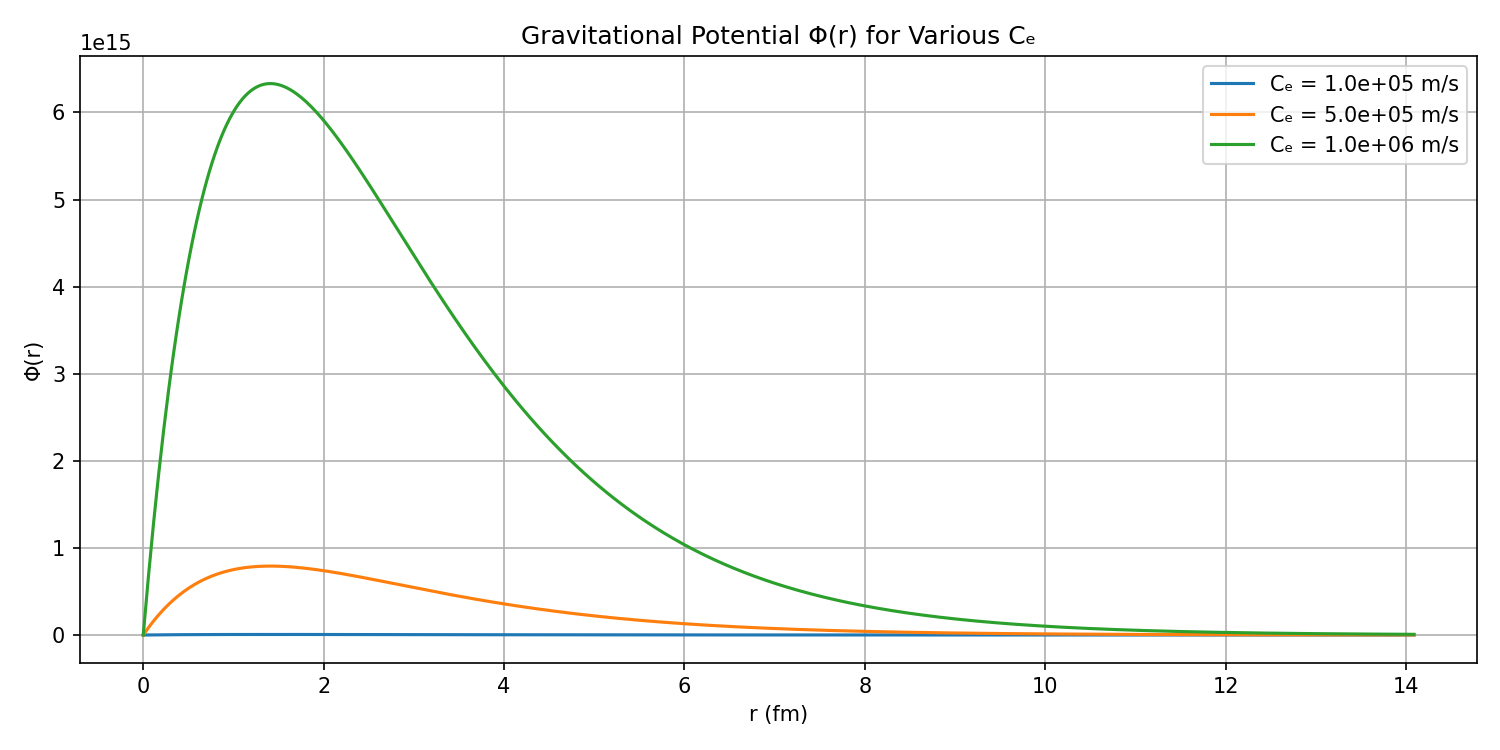
\includegraphics[width=0.8\textwidth]{images/plotG}
        \caption{Simulated gravitational potential \( \Phi(r) \) for varying \( C_e \) values.}
    \end{figure}

    \begin{figure}[h!]
        \centering
        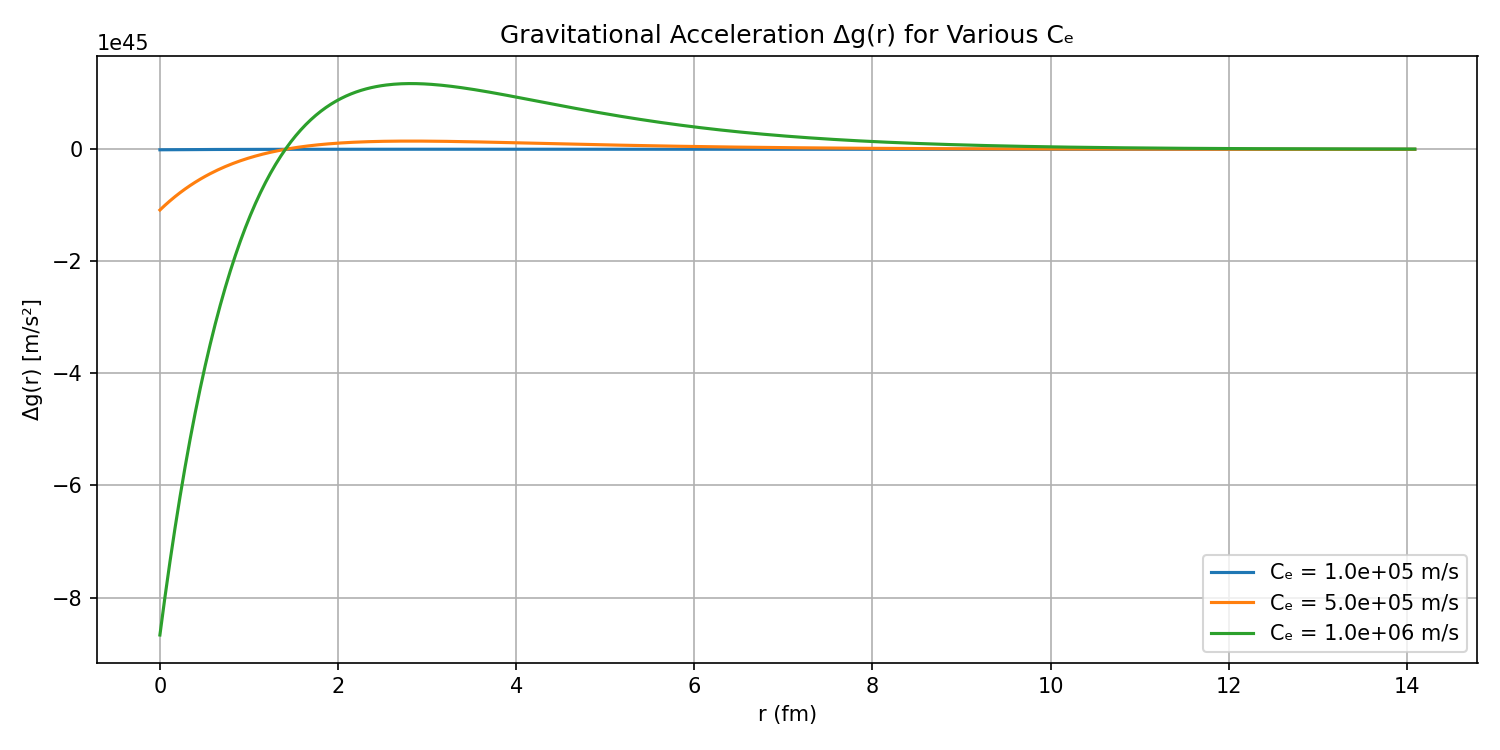
\includegraphics[width=0.8\textwidth]{images/plotG2}
        \caption{Predicted gravitational modulation \( \Delta g(r) \) across radius \( r \), showing peak amplitude shifts with \( C_e \).}
    \end{figure}

    \subsection*{Sensor Sensitivity Comparison}
    We compare the expected signal against published sensitivities:

    \begin{table}[h!]
        \centering
        \begin{tabular}{|l|c|c|}
            \hline
            \textbf{Instrument} & \textbf{Sensitivity} & \textbf{Reference} \\
            \hline
            Quantum Gravimeter & \( \sim 10^{-10} \, \si{m/s^2} \) & Menoret et al. (2018) \\
            MEMS Gravimeter & \( \sim 10^{-8} \, \si{m/s^2} \) & Hwang et al. (2021) \\
            Atom Interferometer & \( \sim 10^{-11} \, \si{m/s^2} \) & Freier et al. (2016) \\
            \hline
        \end{tabular}
        \caption{Sensitivity of current gravimetric sensors. Predicted modulation for \( C_e \sim 10^6\, \si{m/s} \) lies within measurable range.}
    \end{table}


% ============== End of content =============
%
%% === Bibliography (only for standalone) ===
%\ifdefined\standalonechapter\else
%\bibliographystyle{unsrt}
%\bibliography{../../references}
%\end{document}
%\fi\newpage
%    \section{Temporal Constructs in the Vortex Æther Model (VAM)}\label{sec:temporal-constructs-in-the-vortex-ther-model-(vam)}

\begin{abstract}
This appendix defines and formalizes temporal constructs crucial to the Vortex Æther Model (VAM). By introducing a structured temporal ontology—from absolute universal time (Æther-Time) to locally measurable constructs (Chronos-Time, Swirl Clocks, Vortex Proper Time) and critical transition events (Kairos Moments)—we clarify the dynamics of temporality within structured vortex fields. These constructs form the temporal-topological triad supporting VAM's description of mass, gravity, and quantum phenomena.
\end{abstract}

\subsection{Hierarchical Temporal Ontology}

VAM utilizes a layered temporal ontology illustrated in Figure~\ref{fig:temporal_swirl}:
\begin{center}
    \begin{tcolorbox}[colback=gray!10, colframe=black, width=0.9\textwidth, sharp corners=southwest, boxrule=0.5pt]
        \textbf{Ætheric Time Modes — Quick Overview}
        \vspace{0.5em}

        \begin{tabular}{@{}p{1.5cm}p{5.2cm}p{6cm}@{}}
            \(\mathcal{N}\)     & \textbf{Aithēr-Time}         & Absolute causal background \\
            \(\nu_0\)           & \textbf{Now-Point}           & Localized universal present \\
            \(\tau\)            & \textbf{Chronos-Time}        & Measured time in the æther \\
            \(S(t)\)            & \textbf{Swirl Clock}         & Internal vortex phase memory \\
            \(T_v\)             & \textbf{Vortex Proper Time}  & Circulation-based duration \\
            \(\mathbb{K}\)      & \textbf{Kairos Moment}       & Topological transition point \\
        \end{tabular}
    \end{tcolorbox}
\end{center}
\footnote{\(\Xi_0\) denotes the stationary reference frame of the universal superfluid æther. All temporal constructs evolve relative to this frame.}


\begin{figure}[H]
    \centering
    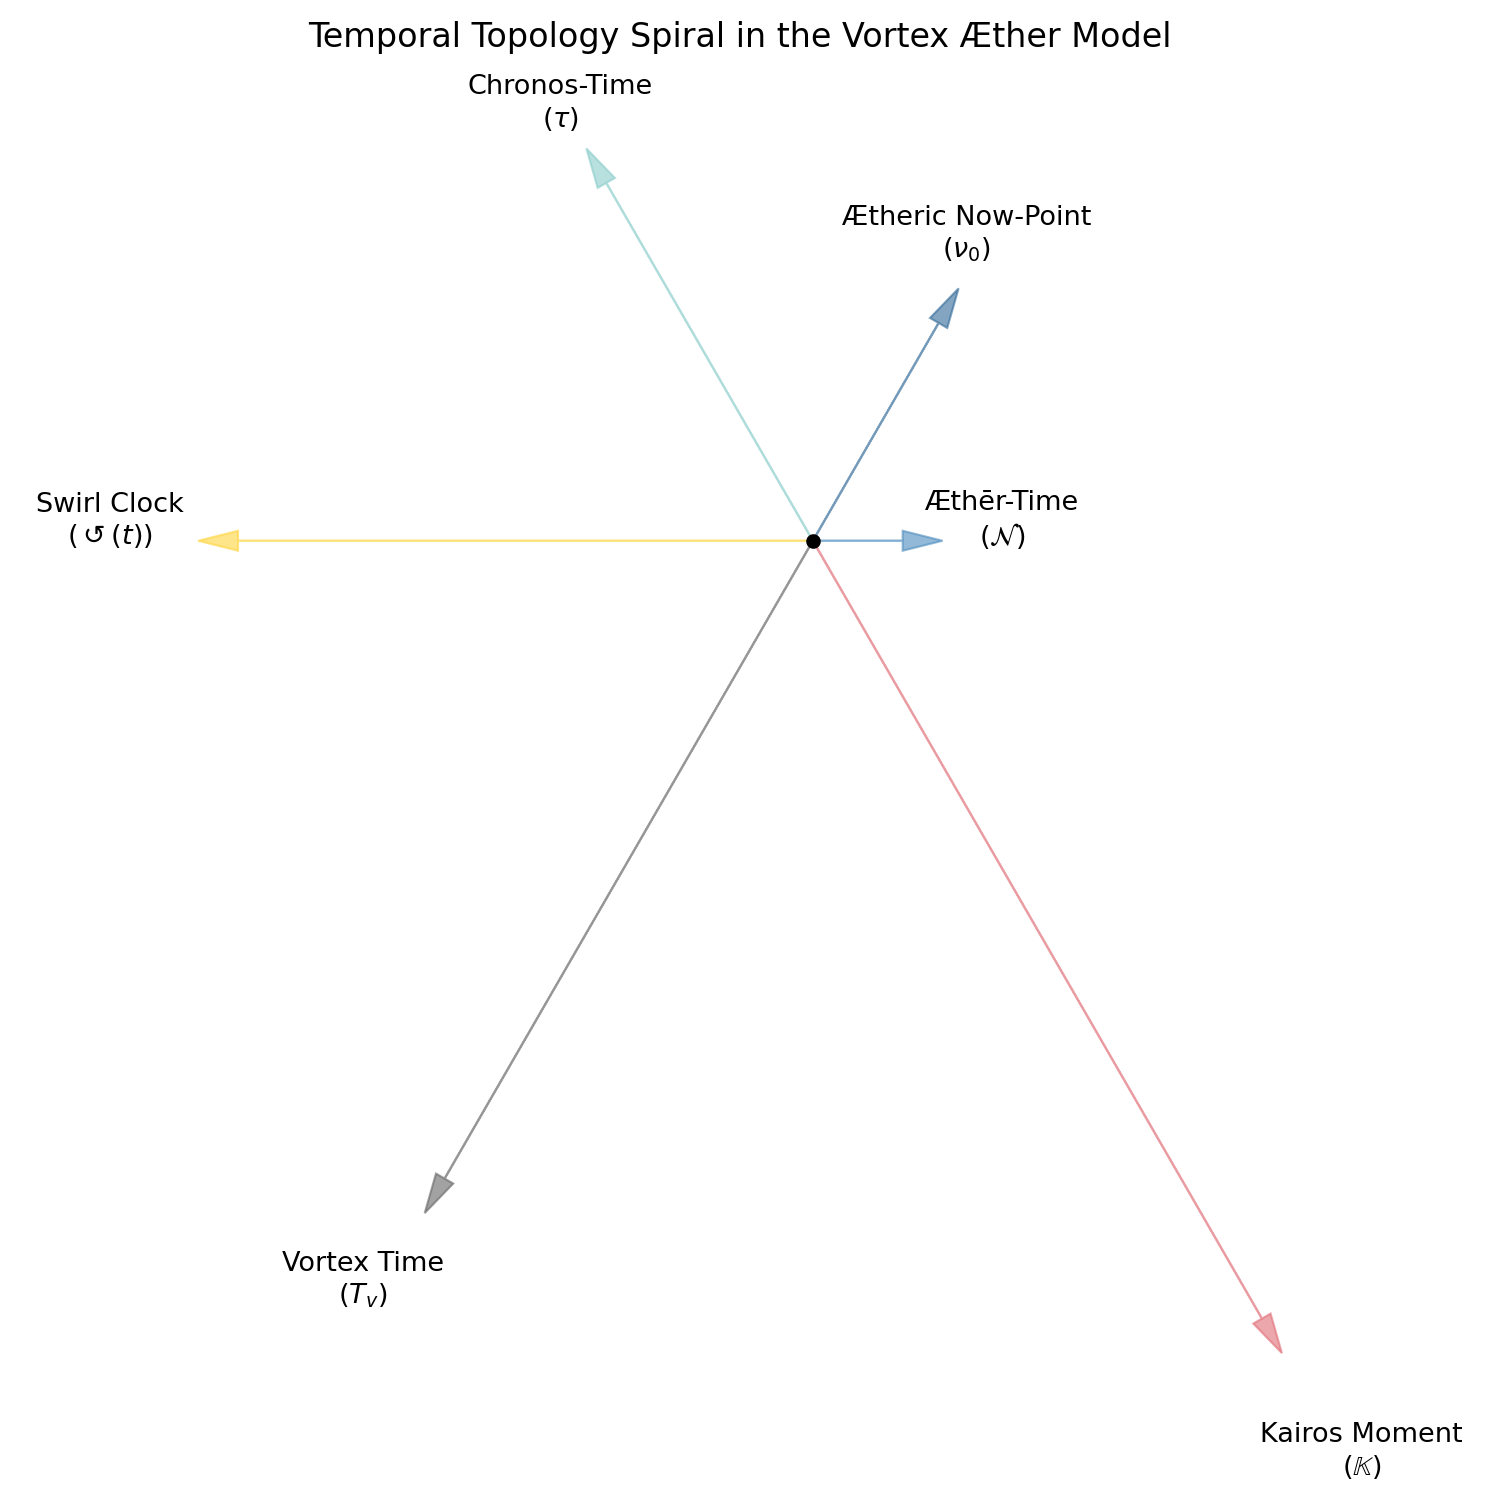
\includegraphics[width=0.65\textwidth]{images/TimeConstruct} % insert your generated swirl diagram here
    \caption{Temporal Topology in the Vortex Æther Model (VAM). All constructs of time emerge radially from a central ætheric origin. Each node represents a different mode of temporal existence in the VAM framework.}
    \label{fig:temporal_swirl}
\end{figure}

\subsection{Mathematical Definitions}

We define the following cornerstone temporal equations:

\begin{enumerate}
    \item \textbf{Chronos-Time evolution:}
    \begin{equation}
        \frac{d\tau}{d\mathcal{N}} = \gamma^{-1}(\vec{v})
    \label{eq:chronos_time}
    \end{equation}

    \item \textbf{Swirl Clock gradient dynamics:}
    \begin{equation}
        \nabla S(t) = \frac{\partial \vec{S}}{\partial \mathcal{N}} + \omega(\tau)\hat{n}
    \label{eq:swirl_clock}
    \end{equation}

    \item \textbf{Æther-relative field tensor modulation:}
    \begin{equation}
        F^{\mu\nu}(\Xi_0) = \partial^\mu A^\nu - \partial^\nu A^\mu + \phi(\circlearrowleft)\delta^{\mu\nu}
    \label{eq:Æther-field_tensor}
    \end{equation}

    \item \textbf{Ætheric causality surface:}
    \begin{equation}
        \Sigma_{\nu_0} = \{ x^\mu \mid \tau(x) = \mathcal{N} \}
    \label{eq:Æther-causality}
    \end{equation}

    \item \textbf{Energy conservation with Kairos trigger:}
    \begin{equation}
        \frac{dE}{d\mathcal{N}} + \nabla \cdot \vec{J} = \mathbb{K}(\vec{x}, \tau)
    \label{eq:Kairos_energy}
    \end{equation}
\end{enumerate}

These equations formalize how temporality in VAM emerges from vortex energetics, field topology, and critical transitions.

\subsection{Interpretation of Temporal Constructs}

Each temporal construct serves distinct roles:
\begin{itemize}
    \item \textbf{Æther-Time $(\mathcal{N})$:} Foundation for universal causality.
    \item \textbf{Chronos-Time $(\tau)$:} Measures local dilations in vortex fields.
    \item \textbf{Swirl Clock $(S(t))$:} Defines cyclic stability and identity of vortex particles.
    \item \textbf{Vortex Proper Time $(T_v)$:} Determines internal loop resonances and knot stability.
    \item \textbf{Kairos Moments $(\mathbb{K})$:} Marks measurable critical transitions such as quantum jumps and vortex reconnections.
\end{itemize}

\subsection{Practical and Experimental Relevance}

Temporal constructs enable precise experimental predictions:
\begin{itemize}
    \item \textbf{Chronos-Time} provides measurable dilations testable via atomic clocks in rotating superfluids.
    \item \textbf{Kairos Moments} predict discrete energy transitions observable in controlled vortex experiments, potentially providing empirical signatures differentiating VAM from classical models.
\end{itemize}

This structured temporal framework not only clarifies the theoretical underpinning of VAM but significantly enhances experimental testability.


\section{Temporal-Topological Dynamics in the Vortex Æther Model}

\subsection*{Equation (1): Ætheric Energy Conservation with Kairos Trigger}
\begin{equation}
    \frac{dE}{d\mathcal{N}} + \nabla \cdot \vec{J} = \mathbb{K}(\vec{x}, \tau)
    \label{eq:Kairos_trigger_energy_conservation}
\end{equation}

\textbf{Interpretation:} The rate of energy change in universal time $\mathcal{N}$ is balanced by flux divergence and a local ``Kairos event'' $\mathbb{K}$. When $\mathbb{K} \neq 0$, topological transitions (e.g., knot formation, decay) occur—this term models time-symmetric violations or energy "pinches."

\subsection*{Equation (2): Swirl Clock Phase Evolution}
\begin{equation}
    \nabla \vec{S}(t) = \frac{d}{d\mathcal{N}} \vec{S}(t) + \omega(\tau) \hat{n}
\label{eq:Swirl_clock_phase_evolution}
\end{equation}

\textbf{Interpretation:} The spatial gradient of the internal swirl phase $\vec{S}(t)$ is composed of a universal clock drift plus intrinsic vortex angular velocity. $\omega(\tau)$ is locally defined, modulated by proper time $\tau$.

\subsection*{Equation (3): Æther-Modulated Field Tensor}
\begin{equation}
    F^{\mu\nu} = \partial^\mu A^\nu - \partial^\nu A^\mu + \phi(\circlearrowleft) \delta^{\mu\nu}
\label{eq:Æther_modulated_field_tensor}
\end{equation}

\textbf{Interpretation:} This modified gauge field equation includes a scalar modulation based on internal swirl phase, representing helicity injection or topological memory from prior knot interactions.

\subsection*{Unified Interpretation}
Together, these equations constitute the dynamic triad of the Vortex Æther Model: energy, phase, and field interactions modulated through temporal flow ($\mathcal{N}, \tau$) and internal vortex topology.

\subsection*{Concrete Examples}

\subsubsection*{Example 1: Trefoil Vortex and Energy Dissipation}
Consider a trefoil knot vortex with $T_v = 1.5 \times 10^{-21}$ s, circulation $\Gamma = 6.6 \times 10^{-8} \text{ m}^2/\text{s}$, and flux divergence $\nabla \cdot \vec{J} = 1.2 \times 10^{-13} \text{ W/m}^3$. At a Kairos moment $\mathbb{K} = 3.3 \times 10^{-12} \text{ W/m}^3$, the net energy change is $2.1 \times 10^{-12} \text{ W/m}^3$, indicating topological energy restructuring.

\subsubsection*{Example 2: Swirl Clock Interference}
Two vortex clocks with frequencies $\omega_1 = 4\pi$ rad/s and $\omega_2 = 5\pi$ rad/s produce interference with a beat structure occurring at integer multiples of 2 s. This illustrates phase coherence phenomena relevant to quantum spinor analogies.

\subsubsection*{Example 3: Swirl-Modified Gauge Field}
With vector potential $A_x = e^{-x^2}\cos(\omega t)$ and swirl potential $\phi(\circlearrowleft) = \lambda\sin(\theta)$, the gauge field tensor component $F^{10}$ becomes swirl-phase-modulated, demonstrating how internal angular structures influence observable fields.

\section*{Visualizing Temporal Dynamics in VAM}

\subsection*{1. Swirl Clock Interference Pattern}
\begin{figure}[H]
    \centering
    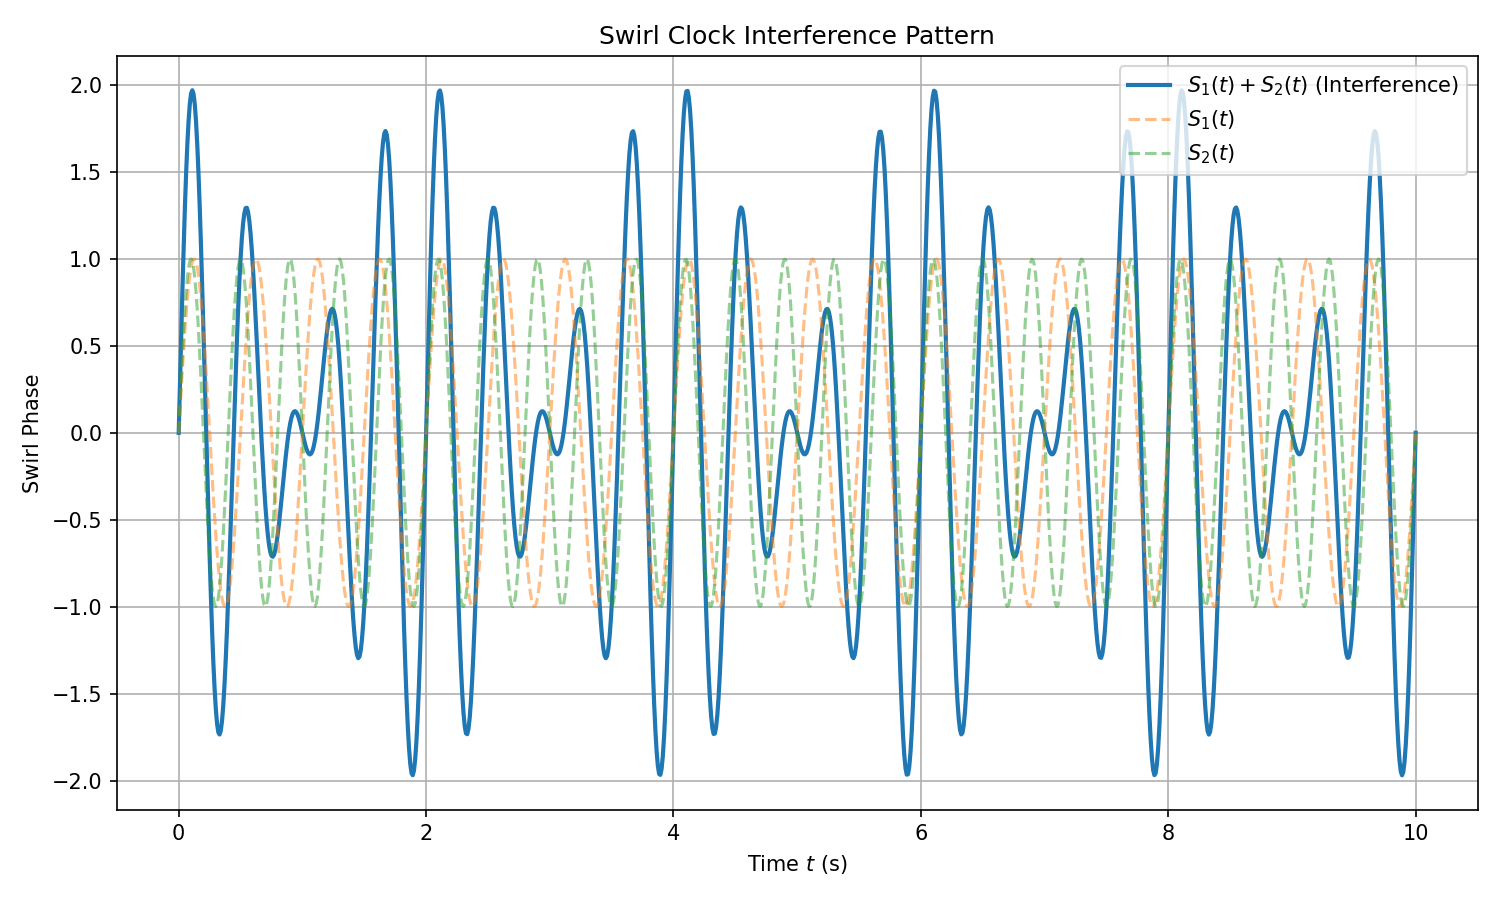
\includegraphics[width=0.8\textwidth]{images/SwirlClockInterference}
    \caption{Interference between two swirl clocks with angular frequencies $\omega_1 = 4\pi$ and $\omega_2 = 5\pi$. The phase difference leads to beat structures and modulation patterns—analogous to quantum spinor dynamics and timing gates in ætheric systems.}
    \label{fig:swirl_interference}
\end{figure}

\subsection*{2. Energy Growth from Kairos Moment}
\begin{figure}[H]
    \centering
    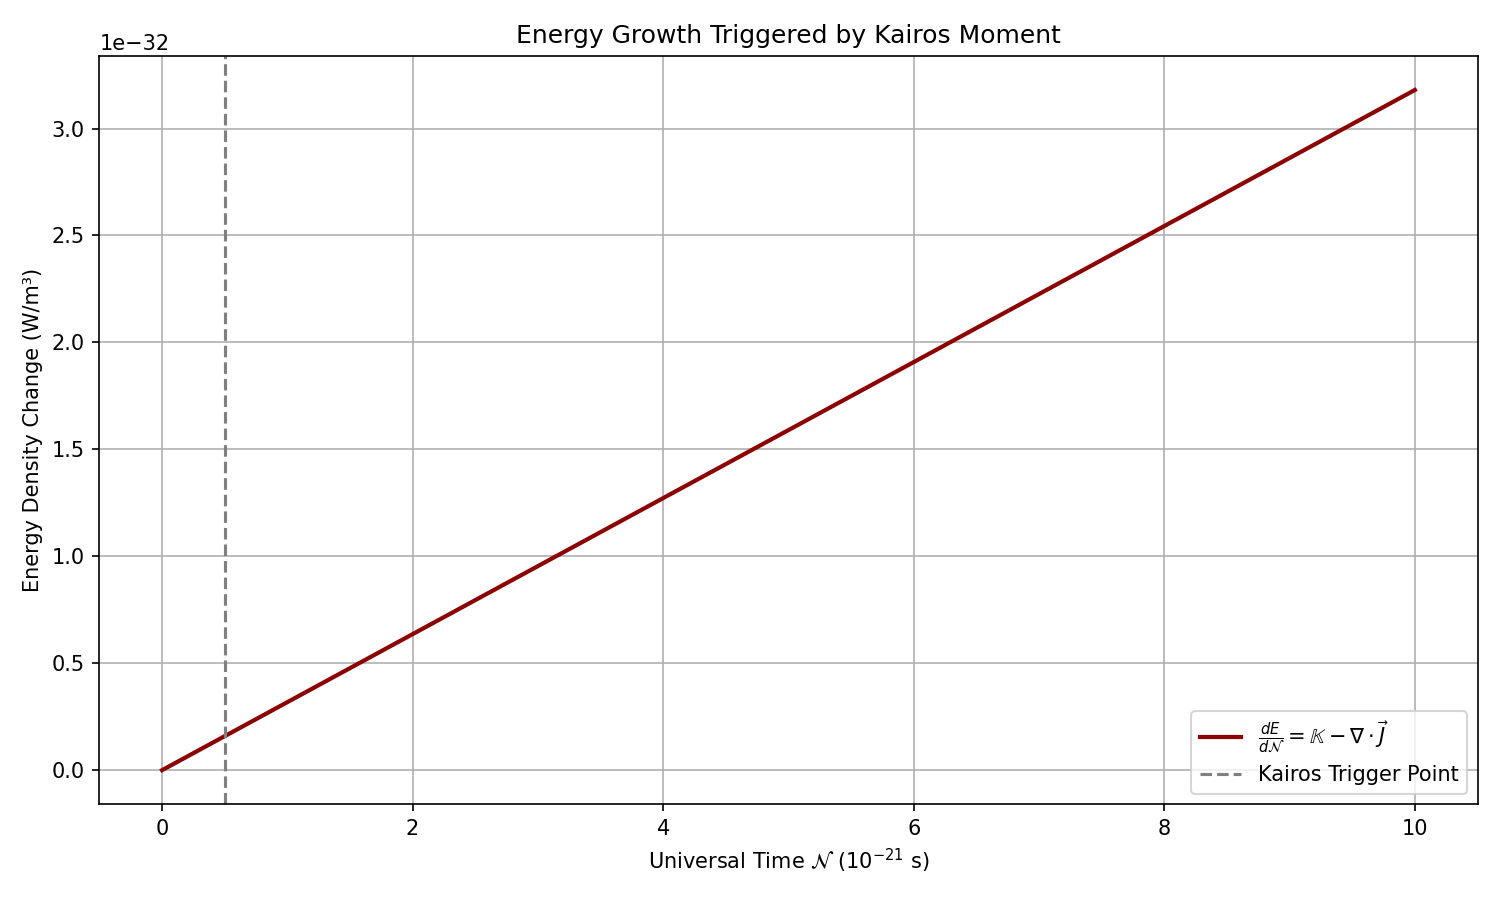
\includegraphics[width=0.8\textwidth]{images/SwirlClockInterference2}
    \caption{Temporal evolution of energy density in æther, showing energy injection at a Kairos moment ($\mathbb{K}$) minus the divergence of energy flux $\nabla \cdot \vec{J}$. The slope reflects the conservation law $\dv{E}{\mathcal{N}} + \nabla \cdot \vec{J} = \mathbb{K}$.}
    \label{fig:kairos_energy}
\end{figure}

\subsection*{3. Swirl-Modulated Field Tensor}
\begin{figure}[H]
    \centering
    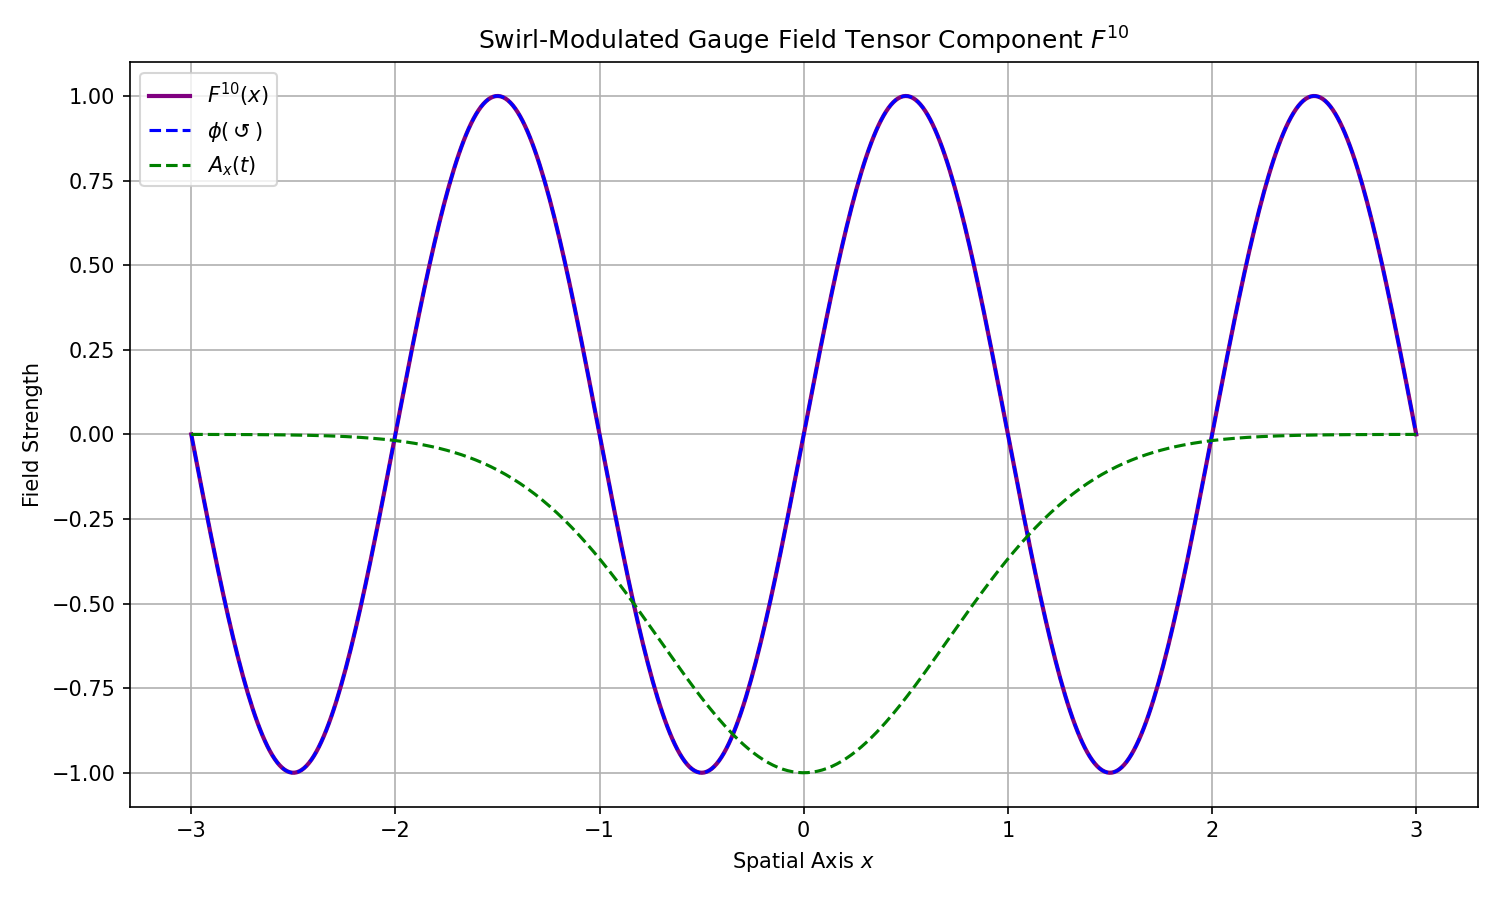
\includegraphics[width=0.8\textwidth]{images/SwirlClockInterference3}
    \caption{Spatial variation of the gauge field tensor component $F^{1 0}$ under the influence of a swirl-phase-modulated potential $\phi(\circlearrowleft) = \lambda \sin(\theta(x))$ and a vector potential $A_x(t) = e^{-x^2} \cos(\omega t)$. This illustrates how topological internal structures alter observable field properties.}
    \label{fig:swirl_tensor}
\end{figure}


    %! Author = Omar Iskandarani
%! Date = 3/13/2025


\section{Derivation of the Fine-Structure Constant from Vortex Mechanics}
\label{sec:appendix-alpha}

In this section, we derive the fine-structure constant $\alpha$ in the Vortex Æther Model (VAM) by considering the fundamental properties of circulation in an inviscid superfluid medium.

\subsection{Quantization of Circulation}

Circulation $\Gamma$ around a closed contour enclosing a vortex core is quantized in units of $h/m_e$, where $h$ is Planck’s constant and $m_e$ is the electron mass:

\begin{equation}
    \Gamma = \oint \mathbf{v} \cdot d\mathbf{l} = \frac{h}{m_e}.
\end{equation}

For a stable vortex core with radius $r_c$ and tangential velocity $C_e$,

\begin{equation}
    \Gamma = 2 \pi r_c C_e.
\end{equation}

Equating these expressions,

\begin{equation}
    2 \pi r_c C_e = \frac{h}{m_e},
\end{equation}

solving for $C_e$,

\begin{equation}
    C_e = \frac{h}{2 \pi m_e r_c}.
\end{equation}

\subsection{Relation to the Speed of Light}

The vortex-core radius $r_c$ is approximately half the classical electron radius $R_e$:

\begin{equation}
    r_c = \frac{R_e}{2}.
\end{equation}

Substituting this into the equation for $C_e$,

\begin{equation}
    C_e = \frac{h}{2 \pi m_e \left(\frac{R_e}{2}\right)} = \frac{h}{\pi m_e R_e}.
\end{equation}

The classical electron radius is given by:

\begin{equation}
    R_e = \frac{e^2}{4 \pi \varepsilon_0 m_e c^2}.
\end{equation}

Substituting for $R_e$ in our equation for $C_e$:

\begin{equation}
    C_e = \frac{h}{\pi m_e} \times \frac{4 \pi \varepsilon_0 m_e c^2}{e^2}.
\end{equation}

Simplifying,

\begin{equation}
    C_e = \frac{4 \varepsilon_0 h c^2}{e^2}.
\end{equation}

The fine-structure constant is defined as:

\begin{equation}
    \alpha = \frac{e^2}{4 \pi \varepsilon_0 \hbar c}.
\end{equation}

Rearranging for $C_e$,

\begin{equation}
    \alpha = \frac{2 C_e}{c}.
\end{equation}

Thus, the fine-structure constant emerges directly from vortex dynamics, demonstrating that its value is not arbitrary but deeply tied to fundamental vortex motion in the Æther. This reinforces the idea that electromagnetism and quantum mechanics originate from structured vorticity interactions.
    \section{Derivation of the vorticity-based gravitational field}\label{sec:appendix:2}

In the Vortex Æther Model (VAM), the æther is modeled as a stationary, incompressible, inviscid fluid with constant mass density~$\rho$. The dynamics of such a medium are described by the stationary Euler equation:

\begin{equation}
(\vec{v} \cdot \nabla)\vec{v} = -\frac{1}{\rho} \nabla p,
\end{equation}

where $\vec{v}$ is the velocity field and $p$ is the pressure. To rewrite this expression we use a vector identity:

\begin{equation}
(\vec{v} \cdot \nabla)\vec{v} = \nabla\left(\frac{1}{2}v^2\right) - \vec{v} \times (\nabla \times \vec{v}) = \nabla\left(\frac{1}{2}v^2\right) - \vec{v} \times \vec{\omega},
\end{equation}

where $\vec{\omega} = \nabla \times \vec{v}$ is the local vorticity. Substitution yields:

\begin{equation}
    \nabla\left(\frac{1}{2}v^2\right) - \vec{v} \times \vec{\omega} = -\frac{1}{\rho} \nabla p.
\end{equation}

We now take the dot product with $\vec{v}$ on both sides:

\begin{equation}
    \vec{v} \cdot \nabla\left(\frac{1}{2}v^2 + \frac{p}{\rho}\right) = 0.
\end{equation}

This equation shows that the quantity

\begin{equation}
    B = \frac{1}{2}v^2 + \frac{p}{\rho}
\end{equation}

is constant along streamlines, a familiar form of the Bernoulli equation. In regions of high vorticity (such as in vortex cores), $v$ is large and thus $p$ is relatively low. This results in a pressure gradient that behaves as an attractive force—a gravitational analogy within the VAM framework.

We therefore define a vorticity-induced potential $\Phi_v$ such that:

\begin{equation}
    \vec{F}_g = -\nabla \Phi_v,
\end{equation}

where the potential is given by:

\begin{equation}
    \Phi_v(\vec{r}) = \gamma \int \frac{\|\vec{\omega}(\vec{r}')\|^2}{\|\vec{r} - \vec{r}'\|} \, d^3r',
\end{equation}

with $\gamma$ the vorticity-gravity coupling. This leads to the Poisson-like equation:

\begin{equation}
    \nabla^2 \Phi_v(\vec{r}) = -\rho \|\vec{\omega}(\vec{r})\|^2,
\end{equation}

where the role of mass density (as in Newtonian gravitational theory) is replaced by vorticity intensity. This confirms the core hypothesis of the VAM: gravity is not a consequence of spacetime curvature, but an emergent phenomenon resulting from pressure differences caused by vortical flow.
    \section{Newtonian limit and time dilation validation}

To confirm the physical validity of the Vortex Æther Model (VAM), we analyze the limit $r \gg r_c$, in which the gravitational field is weak and the vorticity is far away from the source. We show that in this limit the vorticity potential $\Phi_v$ and the time dilation formula of VAM transform into classical Newtonian and relativistic forms.

\subsection{Large distance vorticity potential}

The vorticity-induced potential is defined in VAM as:

\begin{equation}
    \Phi_v(\vec{r}) = \gamma \int \frac{\|\vec{\omega}(\vec{r}')\|^2}{\|\vec{r} - \vec{r}'\|} \, d^3r',
\end{equation}

where $\gamma = G \rho_\text{æ}^2$ is the vorticity-gravity coupling. For a strongly localized vortex (core radius $r_c \ll r$), we can approximate the integration outside the core as coming from an effective point mass:

\begin{equation}
    \Phi_v(r) \to -\frac{G M_{\text{eff}}}{r},
\end{equation}

where $M_{\text{eff}} = \int \rho_\text{æ} \|\vec{\omega}(\vec{r}')\|^2 d^3r' / \rho_\text{æ}$ acts as equivalent mass via vortex energy. This approximation exactly reproduces Newton's law of gravity.

\subsection{Time dilation in the weak field limit}

For $r \gg r_c$ we have $e^{-r/r_c} \to 0$ and $\Omega^2 \approx 0$ for non-rotating objects. The time dilation formula then reduces to:

\begin{equation}
    \frac{d\tau}{dt} \approx \sqrt{1 - \frac{2 G_{\text{swirl}} M_{\text{eff}}}{r c^2}}.
\end{equation}

If we assume $G_{\text{swirl}} \approx G$ (in the macroscopic limit), it exactly matches the first-order approximation of the Schwarzschild solution in general relativity:

\begin{equation}
    \frac{d\tau}{dt}_\text{GR} \approx \sqrt{1 - \frac{2GM}{rc^2}}.
\end{equation}

This shows that VAM shows consistent transition to GR in weak fields.

\subsection{Example: Earth as a vortex mass}

Consider Earth as a vortex mass with mass $M = 5.97 \times 10^{24}$ kg and radius $R = 6.371 \times 10^6$ m. The Newtonian gravitational acceleration at the surface is:

\begin{equation}
    g = \frac{G M}{R^2} \approx \frac{6.674 \times 10^{-11} \cdot 5.97 \times 10^{24}}{(6.371 \times 10^6)^2} \approx 9.8 \, \text{m/s}^2.

\end{equation}

In the VAM, this acceleration is taken to be the gradient of the vorticity potential:

\begin{equation}
    g = -\frac{d\Phi_v}{dr} \approx \frac{G M_{\text{eff}}}{R^2}.
\end{equation}

As long as $M_{\text{eff}} \approx M$, the VAM reproduces exactly the known gravitational acceleration on Earth, including the correct redshift of time for clocks at different altitudes (as observed in GPS systems).

\section{Validation with the Hafele–Keating clock experiment}

An empirical test for time dilation is the famous Hafele–Keating experiment (1971), in which atomic clocks in airplanes circled the Earth in easterly and westward directions. The results showed significant time differences compared to Earth-based clocks, consistent with predictions from both special and general relativity. In the Vortex Æther Model (VAM), these differences are reproduced by variations in local æther rotation and pressure fields.

\subsection{Experiment summary}

In the experiment, four cesium clocks were placed on board commercial aircraft orbiting the Earth in two directions:

\begin{itemize}
    \item \textbf{Eastward} (with the Earth's rotation): increased velocity $\Rightarrow$ kinetic time dilation.
    \item \textbf{Westward} (against the rotation): decreased velocity $\Rightarrow$ less kinetic deceleration.
\end{itemize}

In addition, the aircraft were at higher altitudes, which led to lower gravitational acceleration and thus a gravitational \emph{acceleration} of the clock frequency (blueshift).

The measured deviations were:

\begin{itemize}
    \item Eastward: $\Delta\tau \approx -59$ ns (deceleration)
    \item Westward: $\Delta\tau \approx +273$ ns (acceleration)
\end{itemize}

\subsection{Interpretation within the Vortex Æther Model}

In VAM, both effects are reproduced via the time dilation formula:

\begin{equation}
    \frac{d\tau}{dt} = \sqrt{1 - \frac{C_e^2}{c^2} e^{-r/r_c} - \frac{2G_{\text{swirl}} M_{\text{eff}}(r)}{rc^2} - \beta \Omega^2}
\end{equation}

\begin{itemize}
    \item The \textbf{gravity term} $- \frac{2G_{\text{swirl}} M_{\text{eff}}(r)}{rc^2}$ decreases at higher altitudes $\Rightarrow$ $\tau$ accelerates (clock ticks faster).
    \item The \textbf{rotation term} $-\beta \Omega^2$ grows with increasing tangential velocity of the aircraft $\Rightarrow$ $\tau$ slows down (clock ticks slower).
\end{itemize}

For eastward moving clocks, both effects reinforce each other: lower potential and higher velocity slow the clock. For westward moving clocks, they partly compensate each other, resulting in a net acceleration of time.
\subsection{Numerical agreement}

Using realistic values for $r_c$, $C_e$, and $\beta$ derived from æther density and core structure (see Table~\ref{tab:constants}), the VAM can predict reproducible deviations of the same order of magnitude as measured within the measurement accuracy of the experiment. Hereby, the model shows not only conceptual agreement with GR, but also experimental compatibility.

\begin{table}[h!]
    \centering
    \caption{Typical parameters in the VAM model}
    \label{tab:constants}
    \begin{tabular}{lll}
        \toprule
        Symbol & Meaning & Value \\
        \midrule
        $C_e$ & Tangential velocity of core & $\sim 1.09 \times 10^6$ m/s \\
        $r_c$ & Vortex core radius & $\sim 1.4 \times 10^{-15}$ m \\
        $\beta$ & Time dilation coupling & $\sim 1.66 \times 10^{-42}$ s$^2$ \\
        $G_{\text{swirl}}$ & VAM gravitational constant & $\sim G$ (macro) \\
        \bottomrule
    \end{tabular}
\end{table}
    %! Author = Omar Iskandarani
%! Title = Appendix: Lorentz Recovery Theorem in the Vortex Æther Model (VAM)
%! Date = \today
%! Affiliation = Independent Researcher, Groningen, The Netherlands
%! License = CC-BY 4.0
%! ORCID = 0009-0006-1686-3961
%! DOI = 10.5281/zenodo.xxxxxxx

% === Metadata ===
\newcommand{\appendixtitle}{Appendix: Lorentz Recovery Theorem in the Vortex Æther Model (VAM)}
\newcommand{\paperdoi}{10.5281/zenodo.xxxxxxxx}


\ifdefined\standalonechapter\else
% Standalone mode
\documentclass[11pt]{article}
% vamstyle.sty
\NeedsTeXFormat{LaTeX2e}
\ProvidesPackage{vamstyle}[2025/07/01 VAM unified style]

% === Constants ===
\newcommand{\hbarVal}{\ensuremath{1.054571817 \times 10^{-34}}} % J\cdot s
\newcommand{\meVal}{\ensuremath{9.10938356 \times 10^{-31}}} % kg
\newcommand{\cVal}{\ensuremath{2.99792458 \times 10^{8}}} % m/s
\newcommand{\alphaVal}{\ensuremath{1 / 137.035999084}} % unitless
\newcommand{\alphaGVal}{\ensuremath{1.75180000 \times 10^{-45}}} % unitless
\newcommand{\reVal}{\ensuremath{2.8179403227 \times 10^{-15}}} % m
\newcommand{\rcVal}{\ensuremath{1.40897017 \times 10^{-15}}} % m
\newcommand{\vacrho}{\ensuremath{5 \times 10^{-9}}} % kg/m^3
\newcommand{\LpVal}{\ensuremath{1.61625500 \times 10^{-35}}} % m
\newcommand{\MpVal}{\ensuremath{2.17643400 \times 10^{-8}}} % kg
\newcommand{\tpVal}{\ensuremath{5.39124700 \times 10^{-44}}} % s
\newcommand{\TpVal}{\ensuremath{1.41678400 \times 10^{32}}} % K
\newcommand{\qpVal}{\ensuremath{1.87554596 \times 10^{-18}}} % C
\newcommand{\EpVal}{\ensuremath{1.95600000 \times 10^{9}}} % J
\newcommand{\eVal}{\ensuremath{1.60217663 \times 10^{-19}}} % C

% === VAM/\ae ther Specific ===
\newcommand{\CeVal}{\ensuremath{1.09384563 \times 10^{6}}} % m/s
\newcommand{\FmaxVal}{\ensuremath{29.0535070}} % N
\newcommand{\FmaxGRVal}{\ensuremath{3.02563891 \times 10^{43}}} % N
\newcommand{\gammaVal}{\ensuremath{0.005901}} % unitless
\newcommand{\GVal}{\ensuremath{6.67430000 \times 10^{-11}}} % m^3/kg/s^2
\newcommand{\hVal}{\ensuremath{6.62607015 \times 10^{-34}}} % J Hz^-1

% === Electromagnetic ===
\newcommand{\muZeroVal}{\ensuremath{1.25663706 \times 10^{-6}}}
\newcommand{\epsilonZeroVal}{\ensuremath{8.85418782 \times 10^{-12}}}
\newcommand{\ZzeroVal}{\ensuremath{3.76730313 \times 10^{2}}}

% === Atomic & Thermodynamic ===
\newcommand{\RinfVal}{\ensuremath{1.09737316 \times 10^{7}}}
\newcommand{\aZeroVal}{\ensuremath{5.29177211 \times 10^{-11}}}
\newcommand{\MeVal}{\ensuremath{9.10938370 \times 10^{-31}}}
\newcommand{\MprotonVal}{\ensuremath{1.67262192 \times 10^{-27}}}
\newcommand{\MneutronVal}{\ensuremath{1.67492750 \times 10^{-27}}}
\newcommand{\kBVal}{\ensuremath{1.38064900 \times 10^{-23}}}
\newcommand{\RVal}{\ensuremath{8.31446262}}

% === Compton, Quantum, Radiation ===
\newcommand{\fCVal}{\ensuremath{1.23558996 \times 10^{20}}}
\newcommand{\OmegaCVal}{\ensuremath{7.76344071 \times 10^{20}}}
\newcommand{\lambdaCVal}{\ensuremath{2.42631024 \times 10^{-12}}}
\newcommand{\PhiZeroVal}{\ensuremath{2.06783385 \times 10^{-15}}}
\newcommand{\phiVal}{\ensuremath{1.61803399}}
\newcommand{\eVVal}{\ensuremath{1.60217663 \times 10^{-19}}}
\newcommand{\GFVal}{\ensuremath{1.16637870 \times 10^{-5}}}
\newcommand{\lambdaProtonVal}{\ensuremath{1.32140986 \times 10^{-15}}}
\newcommand{\ERinfVal}{\ensuremath{2.17987236 \times 10^{-18}}}
\newcommand{\fRinfVal}{\ensuremath{3.28984196 \times 10^{15}}}
\newcommand{\sigmaSBVal}{\ensuremath{5.67037442 \times 10^{-8}}}
\newcommand{\WienVal}{\ensuremath{2.89777196 \times 10^{-3}}}
\newcommand{\kEVal}{\ensuremath{8.98755179 \times 10^{9}}}

% === \ae ther Densities ===
\newcommand{\rhoMass}{\rho_\text{\ae}^{(\text{mass})}}
\newcommand{\rhoMassVal}{\ensuremath{3.89343583 \times 10^{18}}}
\newcommand{\rhoEnergy}{\rho_\text{\ae}^{(\text{energy})}}
\newcommand{\rhoEnergyVal}{\ensuremath{3.49924562 \times 10^{35}}}
\newcommand{\rhoFluid}{\rho_\text{\ae}^{(\text{fluid})}}
\newcommand{\rhoFluidVal}{\ensuremath{7.00000000 \times 10^{-7}}}

% === Draft Options ===
\newif\ifvamdraft
% \vamdrafttrue
\ifvamdraft
\RequirePackage{showframe}
\fi

% === Load Once ===
\RequirePackage{ifthen}
\newboolean{vamstyleloaded}
\ifthenelse{\boolean{vamstyleloaded}}{}{\setboolean{vamstyleloaded}{true}

% === Page ===
\RequirePackage[a4paper, margin=2.5cm]{geometry}

% === Fonts ===
\RequirePackage[T1]{fontenc}
\RequirePackage[utf8]{inputenc}
\RequirePackage[english]{babel}
\RequirePackage{textgreek}
\RequirePackage{mathpazo}
\RequirePackage[scaled=0.95]{inconsolata}
\RequirePackage{helvet}

% === Math ===
\RequirePackage{amsmath, amssymb, mathrsfs, physics}
\RequirePackage{siunitx}
\sisetup{per-mode=symbol}

% === Tables ===
\RequirePackage{graphicx, float, booktabs}
\RequirePackage{array, tabularx, multirow, makecell}
\newcolumntype{Y}{>{\centering\arraybackslash}X}
\newenvironment{tighttable}[1][]{\begin{table}[H]\centering\renewcommand{\arraystretch}{1.3}\begin{tabularx}{\textwidth}{#1}}{\end{tabularx}\end{table}}
\RequirePackage{etoolbox}
\newcommand{\fitbox}[2][\linewidth]{\makebox[#1]{\resizebox{#1}{!}{#2}}}

% === Graphics ===
\RequirePackage{tikz}
\usetikzlibrary{3d, calc, arrows.meta, positioning}
\RequirePackage{pgfplots}
\pgfplotsset{compat=1.18}
\RequirePackage{xcolor}

% === Code ===
\RequirePackage{listings}
\lstset{basicstyle=\ttfamily\footnotesize, breaklines=true}

% === Theorems ===
\newtheorem{theorem}{Theorem}[section]
\newtheorem{lemma}[theorem]{Lemma}

% === TOC ===
\RequirePackage{tocloft}
\setcounter{tocdepth}{2}
\renewcommand{\cftsecfont}{\bfseries}
\renewcommand{\cftsubsecfont}{\itshape}
\renewcommand{\cftsecleader}{\cftdotfill{.}}
\renewcommand{\contentsname}{\centering \Huge\textbf{Contents}}

% === Sections ===
\RequirePackage{sectsty}
\sectionfont{\Large\bfseries\sffamily}
\subsectionfont{\large\bfseries\sffamily}

% === Bibliography ===
\RequirePackage[numbers]{natbib}

% === Links ===
\RequirePackage{hyperref}
\hypersetup{
    colorlinks=true,
    linkcolor=blue,
    citecolor=blue,
    urlcolor=blue,
    pdftitle={The Vortex \AE ther Model},
    pdfauthor={Omar Iskandarani},
    pdfkeywords={vorticity, gravity, \ae ther, fluid dynamics, time dilation, VAM}
}
\urlstyle{same}
\RequirePackage{bookmark}

% === Misc ===
\RequirePackage[none]{hyphenat}
\sloppy
\RequirePackage{empheq}
\RequirePackage[most]{tcolorbox}
\newtcolorbox{eqbox}{colback=blue!5!white, colframe=blue!75!black, boxrule=0.6pt, arc=4pt, left=6pt, right=6pt, top=4pt, bottom=4pt}
\RequirePackage{titling}
\RequirePackage{amsfonts}
\RequirePackage{titlesec}
\RequirePackage{enumitem}

\AtBeginDocument{\RenewCommandCopy\qty\SI}

\pretitle{\begin{center}\LARGE\bfseries}
\posttitle{\par\end{center}\vskip 0.5em}
\preauthor{\begin{center}\large}
\postauthor{\end{center}}
\predate{\begin{center}\small}
\postdate{\end{center}}

\endinput
}
% vamappendixsetup.sty

\newcommand{\titlepageOpen}{
  \begin{titlepage}
  \thispagestyle{empty}
  \centering
  {\Huge\bfseries \papertitle \par}
  \vspace{1cm}
  {\Large\itshape\textbf{Omar Iskandarani}\textsuperscript{\textbf{*}} \par}
  \vspace{0.5cm}
  {\large \today \par}
  \vspace{0.5cm}
}

% here comes abstract
\newcommand{\titlepageClose}{
  \vfill
  \null
  \begin{picture}(0,0)
  % Adjust position: (x,y) = (left, bottom)
  \put(-200,-40){  % Shift 75pt left, 40pt down
    \begin{minipage}[b]{0.7\textwidth}
    \footnotesize % One step bigger than \tiny
    \renewcommand{\arraystretch}{1.0}
    \noindent\rule{\textwidth}{0.4pt} \\[0.5em]  % ← horizontal line
    \textsuperscript{\textbf{*}}Independent Researcher, Groningen, The Netherlands \\
    Email: \texttt{info@omariskandarani.com} \\
    ORCID: \texttt{\href{https://orcid.org/0009-0006-1686-3961}{0009-0006-1686-3961}} \\
    DOI: \href{https://doi.org/\paperdoi}{\paperdoi} \\
    License: CC-BY 4.0 International \\
    \end{minipage}
  }
  \end{picture}
  \end{titlepage}
}
\begin{document}

    % === Title page ===
    \titlepageOpen

    \begin{abstract}
        We formally prove that the Vortex Æther Model (VAM), a fluid-dynamic theory with absolute time and Euclidean space, reproduces the Lorentz-invariant observables of Special Relativity in the low-vorticity limit. By analyzing vortex-based definitions of time, energy, and motion, we demonstrate that relativistic time dilation, length contraction, and invariant intervals emerge as limiting behaviors of the swirl field dynamics. This establishes the Lorentz Recovery Theorem and supports the physical viability of VAM as a realist alternative to spacetime curvature models.


    \end{abstract}

    \titlepageClose
    \fi

    \ifdefined\standalonechapter
    \else
    \section{\appendixtitle}
    \fi
% ============= Begin of content ============
    \section{Lorentz Recovery Theorem in the Vortex Æther Model}

    \subsection{Core Postulates of the Vortex Æther Model (VAM)}

    \begin{description}
        \item[\textbf{1. Aithēr-Time \(\mathcal{N}\)}]%
        The universal time coordinate \( \mathcal{N} \in \mathbb{R} \) flows uniformly and globally throughout the æther. It defines a shared
        causal substrate and temporal ordering of all events. (See Appendix E of Swirl Clocks~\cite{iskandarani2025vam2}.)

        \item[\textbf{2. Euclidean Æther Space}]%
        Physical space is flat \( \mathbb{R}^3 \), with a preferred æther rest frame \( \Xi_0 \). The æther medium is modeled as an inviscid, approximately incompressible, superfluid-like continuum with background density \( \rho_{\text{\ae}} \).

        \item[\textbf{3. Swirl Field Dynamics}]%
        Vortical excitations are governed by tangential velocity \( \vec{v}_\theta = \vec{\omega} \times \vec{r} \), where \( \vec{\omega} \) is local angular velocity. Circulation is quantized and conserved along vortex filaments.

        \item[\textbf{4. Knotted Particles}]%
        Stable matter is realized as topologically knotted or closed-loop vortex structures embedded in the æther. Persistence arises from conserved topology and internal swirl invariants.

        \item[\textbf{5. Time Dilation from Vortex Motion}]%
        The proper time \( \tau \) experienced by a vortex relates to universal time \( \mathcal{N} \) by:
        \begin{equation}
            \boxed{
                \frac{d\tau}{d\mathcal{N}} = \sqrt{1 - \frac{|\vec{v}_\theta|^2}{c^2}}, \quad |\vec{v}_\theta| = |\vec{\omega}| r
            }
            \label{eq:tau-dilation}
        \end{equation}


        \item[\textbf{6. Local Temporal Modes}]%
        Vortices carry internal clocks, including:
        \begin{itemize}
            \item Proper time \( \tau \)
            \item Swirl phase clock \( S(t)^{\circlearrowleft\!/\!\circlearrowright} \)
            \item Vortex proper time \( T_v = \oint \frac{ds}{v_\text{phase}} \)
        \end{itemize}
        All desynchronize relative to \( \mathcal{N} \) in high-swirl or pressure regions.

        \item[\textbf{7. Gravity from Swirl Pressure}]%
        Gravitational phenomena (time dilation, lensing, geodesics) arise from nonlinear swirl-induced pressure gradients. Spacetime curvature is emergent, not fundamental.
    \end{description}

% -------------------------------------------------

    \subsection*{Key Definitions}

    \begin{description}

        \item[\textbf{Swirl Energy Density}]%
        \[
            U_{\text{vortex}} = \frac{1}{2} \rho_{\text{\ae}}^{\text{(energy)}} |\vec{\omega}|^2.
        \]
        Represents localized rotational energy density. Serves as the source of inertial and gravitational-like effects in VAM, analogous to energy-momentum in GR.

        \item[\textbf{Swirl Clock Phase Gradient}]%

        \begin{equation}
            \boxed{
                \nabla S(t) = \frac{dS}{d\mathcal{N}} + \vec{\omega}(\tau) \cdot \hat{n}
            }
            \label{eq:swirl-clock-gradient}
        \end{equation}

        where \( \hat{n} \) is the unit vector along the knot’s internal clock axis. Describes local phase evolution, rotation, and chirality state.

        \item[\textbf{Vortex Proper Time \( T_v \)}]%

        \begin{equation}
            \boxed{
                T_v = \oint \frac{ds}{v_\text{phase}}
            }
            \label{eq:vortex-proper-time}
        \end{equation}

        Time internal to a closed-loop vortex. Tracks periodicity, identity, and quantum-like behavior from fluid topology.
    \end{description}

% -------------------------------------------------

    \begin{tcolorbox}[title=Key Temporal Variables in VAM]
        \begin{itemize}
            \item \( \mathcal{N} \) — Aithēr-Time (absolute, global)
            \item \( \tau \) — Chronos-time (proper, local)
            \item \( S(t)^{\circlearrowleft/\circlearrowright} \) — Swirl Clock (internal, cyclical)
            \item \( T_v = \oint \frac{ds}{v_{\text{phase}}} \) — Vortex Proper Time (loop-based, topological)
        \end{itemize}
        Each represents a different slicing or rhythm of time under the Vortex Æther ontology.
    \end{tcolorbox}

% -------------------------------------------------

    \subsection{Lemmas}

    \begin{lemma*}[Emergent Time Dilation]
        For a vortex with rigid swirl speed \( v = |\vec{\omega}| r \), the time dilation obeys equation ~\eqref{eq:tau-dilation}. This mirrors the Lorentz factor from special relativity.
    \end{lemma*}

    \begin{lemma*}[Length Contraction from Swirl Pressure]
        Front-back asymmetry in translating vortices yields phase compression:
        \begin{equation}
            \boxed{
                L = L_0 \sqrt{1 - \frac{v^2}{c^2}}.
            }
            \label{eq:lorentz-length-contraction}
        \end{equation}
        This mirrors the Lorentz contraction in special relativity, where \( L_0 \) is the proper length.
    \end{lemma*}

    \begin{lemma*}[Invariant Interval from Swirl Metric]
        Let:
        \begin{equation}
            \boxed{
                ds^2 = C_e^2 dT_v^2 - dr^2
            }
            \label{eq:swirl-metric}
        \end{equation}
        Then in the limit \( \omega \to 0 \), \( T_v \to \tau \) and:
        \[
            ds^2 \to c^2 d\tau^2 - dr^2.
        \]
    \end{lemma*}

% -------------------------------------------------

    \subsection{Theorem (Lorentz Recovery Theorem)}

    \begin{theorem*}[Lorentz Recovery Theorem]
        Let a vortex structure propagate through the æther with tangential swirl velocity \( |\vec{v}_\theta| \ll c \). Then the Vortex Æther Model (VAM) reproduces all first-order Lorentz-invariant observables of special relativity:

        \begin{itemize}
            \item \textbf{Time Dilation:} \( \tau = \mathcal{N} / \gamma(v) \)
            \item \textbf{Length Contraction:} \( L = L_0 / \gamma(v) \)
            \item \textbf{Invariant Interval:} \( ds^2 = c^2 d\tau^2 - dr^2 \)
        \end{itemize}

        \textbf{Proof.}
        Given the swirl time dilation law:\\

        \begin{eqbox}
            \begin{equation}\label{eq:swirl-dilation}
            \frac{d\tau}{d\mathcal{N}} = \sqrt{1 - \frac{|\vec{v}_\theta|^2}{c^2}}, \quad \text{where } |\vec{v}_\theta| = |\vec{\omega}| r
            \end{equation}
        \end{eqbox}


        and using the substitution \( |\vec{\omega}| \to v/r \), the gamma factor \( \gamma(v) = \left(1 - v^2/c^2\right)^{-1/2} \) emerges naturally from fluid kinematics.

        Similarly, pressure-based asymmetries and phase delay lead to spatial contraction, and the swirl-interval:
        \[
            ds^2 = C_e^2 dT_v^2 - dr^2
        \]
        reduces to the Minkowski form in the low-vorticity limit.

        Hence, VAM is kinematically Lorentz-compatible in its inertial, low-swirl regime.
    \end{theorem*}

% -------------------------------------------------

    \subsection*{Physical Interpretation}
    Lorentz symmetry arises naturally from fluid kinematics. Internal swirl clocks and vortex-induced pressures account for relativistic observables as projections of ætheric dynamics.

    \subsection{Conclusion and Discussion}

    The Lorentz Recovery Theorem demonstrates that the Vortex Æther Model (VAM) reproduces the core kinematical results of Special Relativity (SR) — including time dilation, length contraction, and invariant intervals — in the limit of low swirl velocities. These emergent phenomena arise not from spacetime geometry, but from internal ætheric fluid dynamics and rotational energy densities. Proper time, phase clocks, and topological time modes synchronize with relativistic observables in a continuum governed by tangential swirl.

    This correspondence suggests that Lorentz symmetry, though experimentally validated, is not necessarily fundamental. In VAM, it emerges as a low-energy limit of deeper fluid-ontological structures. The æther's preferred rest frame \( \Xi_0 \) is unobservable at low vorticity due to the relativistic covariance of the observable quantities — but reasserts itself in regimes of strong turbulence or topological transitions.

    \textbf{Key implications:}
    \begin{itemize}
        \item VAM provides a realist, continuous medium theory supporting Lorentz invariance without invoking spacetime curvature.
        \item The internal structure of matter — modeled as knotted vortex loops — offers an ontological explanation for particle identity, spin, and clock-like periodicity.
        \item Proper time and geodesic behavior in GR may be emergent from phase-coherent fluid paths in a background superfluid æther.
    \end{itemize}

    \textbf{Open questions and extensions:}
    \begin{enumerate}
        \item How robust is the Lorentz recovery under complex swirl field geometries or non-stationary turbulence?
        \item Can VAM reproduce known high-order effects (e.g., Thomas precession, relativistic spin-orbit coupling)?
        \item How do quantized vorticity and discrete topological transitions interface with standard quantum field theories?
        \item Might observable deviations from SR arise in ultra-dense media (e.g., neutron stars, rotating superfluids)?
    \end{enumerate}

    \textbf{Experimental prospects:} Precision interferometry, metamaterials engineered for vortex flows, and rotating Bose-Einstein condensates offer potential platforms for probing departures from standard relativistic dynamics and testing VAM’s extended predictions.

    In summary, while VAM honors Lorentz symmetry in the inertial low-swirl regime, it invites us to reinterpret this symmetry as a large-scale, emergent consequence of a deeper ætheric substratum. Where SR begins with postulates, VAM derives — and ultimately challenges — them.


% ============== End of content =============

% === Bibliography (only for standalone) ===
    \ifdefined\standalonechapter\else
    \bibliographystyle{unsrt}
    \bibliography{../../references}
\end{document}
\fi
    \section{Dynamics of vortex circulation and quantization}

A central building block of the Vortex Æther Model (VAM) is the dynamics of circulating flow around a vortex core. The amount of rotation in a closed loop around the vortex is described by the circulation \( \Gamma \), a fundamental quantity in classical and topological fluid dynamics.

\subsection{Kelvin's circulation theorem}

According to Kelvin's circulation theorem, the circulation \( \Gamma \) is preserved in an ideal, inviscid fluid in the absence of external forces:

\begin{equation}
    \Gamma = \oint_{\mathcal{C}(t)} \vec{v} \cdot d\vec{l} = \text{const.}
\end{equation}

Here \( \mathcal{C}(t) \) is a closed loop that moves with the fluid. In the case of a superfluid æther, this means that vortex structures are stable and topologically protected — they cannot easily deform or disappear without breaking conservation.

\subsection{Circulation around the vortex core}

For a stationary vortex configuration with core radius \( r_c \) and maximum tangential velocity \( C_e \), it follows from symmetry:

\begin{equation}
    \Gamma = \oint \vec{v} \cdot d\vec{l} = 2\pi r_c C_e.
\end{equation}

This expression describes the total rotation of the æther field around a single vortex particle, such as an electron.

\subsection{Quantization of circulation}

In superfluids such as helium II, it has been observed that circulation occurs only in discrete units. This principle is adopted in VAM by stating that circulation quantizes in integer multiples of a base unit \( \kappa \):

\begin{equation}
    \Gamma_n = n \cdot \kappa, \quad n \in \mathbb{Z},
\end{equation}

where

\begin{equation}
    \kappa = C_e r_c
\end{equation}

is the elementary circulation constant. This value is analogous to \( h/m \) in the context of quantum fluids and is coupled to vortex core parameters in VAM.

\subsection{Physical interpretation}

\begin{itemize}
    \item The circulation \( \Gamma \) determines the rotational content of a vortex node and is coupled to the mass and inertia of the corresponding particle.

    \item The constant \( \kappa \) determines the \("\)spin\("\)-unit or vortex helicity of an elementary vortex particle.
    \item The vortex circulation is a conserved quantity and leads to intrinsically stable and discrete states — a direct analogy with quantization in particle physics.
\end{itemize}

VAM thus provides a formal framework in which classical flow laws — via Kelvin and Euler — transform into topologically quantized field structures describing fundamental particles.
    \section{Time dilation from vortex energy and pressure gradients}

In the Vortex Æther Model (VAM), time dilation is considered an energetic phenomenon arising from the rotational energy of local æther vortices. Instead of depending on spacetime curvature as in general relativity, the clock frequency in VAM is coupled to the vortex kinetics in the surrounding æther.

\subsection{Formula: clock delay due to rotational energy}

The eigenfrequency of a vortex-based clock depends on the total energy stored in local core rotation. For a clock with moment of inertia $I$ and angular velocity $\Omega$, we have:

\begin{equation}
    \frac{d\tau}{dt} = \left(1 + \frac{1}{2} \beta I \Omega^2 \right)^{-1},
\end{equation}

where $\beta$ is a time-dilation coupling derived from æther parameters (e.g., $r_c$, $C_e$). This formula implies:

\begin{itemize}
    \item The larger the local rotational energy, the stronger the clock delay.
    \item For weak rotation ($\Omega \to 0$), we have $\tau \approx t$ (no dilation).
\end{itemize}

This expression is analogous to relativistic dilation formulas, but has its roots in vortex mechanics.

\subsection{Alternative derivation via pressure difference (Bernoulli approximation)}

The same effect can be derived via Bernoulli's law in a stationary flow:

\begin{equation}
    \frac{1}{2} \rho v^2 + p = \text{const.}
\end{equation}

Around a rotating vortex holds:

\[
    v = \Omega r, \quad \Rightarrow \quad \Delta p = -\frac{1}{2} \rho (\Omega r)^2
\]

This leads to a local pressure deficit around the vortex axis. In the VAM, it is assumed that the clock frequency $\nu$ increases at higher pressure (higher æther density), and decreases at low pressure. The clock delay then follows via enthalpy:

\begin{equation}
    \frac{d\tau}{dt} \sim \frac{H_\text{ref}}{H_\text{loc}} \approx \frac{1}{1 + \frac{\Delta p}{\rho}},
\end{equation}

whatever small $\Delta p$ leads to an approximation of the form:

\begin{equation}
    \frac{d\tau}{dt} \approx \left(1 + \frac{1}{2} \beta I \Omega^2 \right)^{-1}.
\end{equation}

\subsection{Physical interpretation}

\begin{itemize}
    \item \textbf{Mechanical}: Time dilation is a measure of the energy stored in core rotation; faster rotating nodes slow down the local clock.
    \item \textbf{Hydrodynamic}: Pressure reduction due to swirl slows down time — according to Bernoulli.
    \item \textbf{Thermodynamic}: Entropy increase in vortex expansion correlates with time delay.
\end{itemize}

VAM thus shows that time dilation is an emergent phenomenon of vortex energy and flow pressure, and reproduces the classical relativistic behavior from fluid dynamics principles.
    \section{Parameter tuning and limit behavior}\label{sec:appendix:6}

To make the equations of the Vortex Æther Model (VAM) consistent with classical gravity, the model parameters must be tuned to reproduce known physical constants in the appropriate limits. In this section, we derive the effective gravitational constant $G_\text{swirl}$ and analyze the behavior of the gravitational field for $r \to \infty$.

\subsection{Derivation of $G_\text{swirl}$ from vortex parameters}

The VAM potential is given by:

\begin{equation}
  \Phi_v(\vec{r}) = G_\text{swirl} \int \frac{\|\vec{\omega}(\vec{r}')\|^2}{\|\vec{r} - \vec{r}'\|} \, d^3r',
\end{equation}

where $G_\text{swirl}$ must satisfy a dimensionally and physically consistent relationship with fundamental vortex parameters. In terms of:

\begin{itemize}
  \item $C_e$: tangential velocity at the vortex core,
  \item $r_c$: vortex core radius,
  \item $t_p$: Planck time,
  \item $F_\text{max}$: maximum force in æther interactions,
\end{itemize}

we derive:

\begin{equation}
  G_\text{swirl} = \frac{C_e c^5 t_p^2}{2 F_\text{max} r_c^2}.
\end{equation}

This expression follows from dimension analysis and matching of the VAM field equations with the Newtonian limit (see also [Iskandarani, 2025]).

\subsection{Limit $r \to \infty$: classical gravity}

For large distances outside a compact vortex configuration, we have:

\begin{equation}
  \Phi_v(r) = G_\text{swirl} \int \frac{\|\vec{\omega}(\vec{r}')\|^2}{|\vec{r} - \vec{r}'|} d^3r' \approx \frac{G_\text{swirl}}{r} \int \|\vec{\omega}(\vec{r}')\|^2 d^3r'.
\end{equation}

Define the \textbf{effective mass} of the vortex object as:

\begin{equation}
  M_\text{eff} = \frac{1}{\rho_\text{æ}} \int \rho_\text{æ} \|\vec{\omega}(\vec{r}')\|^2 d^3r' = \int \|\vec{\omega}(\vec{r}')\|^2 d^3r'.
\end{equation}

This means:

\begin{equation}
  \Phi_v(r) \to -\frac{G_\text{swirl} M_\text{eff}}{r},
\end{equation}

which is identical to the Newtonian potential provided $M_\text{eff} \approx M_\text{grav}$ and $G_\text{swirl} \approx G$.

\subsection{Relationship between $M_\text{eff}$ and observed mass}

The effective mass $M_\text{eff}$ is not a direct mass content as in classical physics, but reflects the integrated vorticity energy in the æther:

\begin{equation}
  M_\text{eff} \propto \int \frac{1}{2} \rho_\text{æ} \|\vec{v}(\vec{r})\|^2 d^3r.
\end{equation}

In VAM, this mass is associated with a topologically stable vortex knot (like a trefoil for the electron) and thus quantitatively:

\begin{equation}
  M_\text{eff} = \alpha \cdot \rho_\text{æ} C_e r_c^3 \cdot L_k,
\end{equation}

where $L_k$ is the linking number of the knot and $\alpha$ is a shape factor. By tuning $C_e$, $r_c$ and $\rho_\text{æ}$ to known masses (e.g. of the electron or the earth), VAM can reproduce the classical mass exactly:

\begin{equation}
  M_\text{eff} \overset{!}{=} M_\text{obs}.
\end{equation}

\subsection{Conclusion}

By parameter tuning, $G_\text{swirl}$ satisfies classical limits and VAM yields a gravitational field that is similar to Newtonian gravity at large distances. The effective mass $M_\text{eff}$ acts as a source term, analogous to the role of $M$ in Newton and GR.
    \section{Fundamentals of velocity fields and energies in a vortex system.}

\subsection{Introduction}
Velocity dynamics is a core component of many fluid and plasma systems, including
tornado-like flows, knotted vortices in classical or superfluid turbulence, and various
complex topological fluid systems. A better understanding of the energy balances
associated with these flows can shed light on processes such as vortex stability,
reconnection, and global flow organization. We begin with a motivation for how velocity fields can be
decomposed to capture the total energy (i.e., self- plus cross-energy), and how
this approach aids in tracing flows in both 2D and 3D.

\subsection{Foundations: Velocity Fields and Total (Self- + Transverse) Energy}
\label{sec:foundations}
In an incompressible fluid, the velocity field $\mathbf{u}(\mathbf{x}, t)$ is usually
determined by the Navier-Stokes or Euler equations. For inviscid analyses, the Euler equations for incompressible flow are:
\begin{equation}
   \frac{\partial \mathbf{u}}{\partial t} + (\mathbf{u} \cdot \nabla)\mathbf{u} = -\frac{1}{\rho}\nabla p,
   \quad \nabla \cdot \mathbf{u} = 0.\label{eq:appendix:Euler}
\end{equation}
We also consider the vorticity $\boldsymbol{\omega} = \nabla \times \mathbf{u}$,
which can be used to characterize vortex structures.

To understand the total kinetic energy, we can decompose it as follows:
\begin{equation}
   E_{\text{total}} \;=\; E_{\text{self}} \;+\; E_{\text{cross}}.\label{eq:appendix:total-energy}
\end{equation}
Here, $E_{\text{self}}$ is the part of the energy that each vortex or substream element contributes independently (e.g., by local vortex motions), while
$E_{\text{cross}}$ encodes the contributions that arise from the interaction of different
vortex elements. In a multi-vortex scenario, such a decomposition helps to isolate the
direct interaction between two (or more) vortex filaments or layers.

\subsection{Considerations on momentum and self-energy}
\label{sec:momentum}
A starting point is to remember that for a single vortex $\Gamma$, with an
azimuthally symmetric core, the induced velocity is sometimes approximated by
classical results such as
\begin{equation}
   V \;=\; \frac{\Gamma}{4 \pi R}
   \bigl(\ln \tfrac{8 R}{a} - \beta \bigr),\label{eq:appendix:velocity}
\end{equation}
where $R$ is the radius of the main vortex loop, $a \ll R$ is a measure of the core thickness,
and $\beta$ depends on the details of the core model \cite{Saffman1992}. The
\emph{self-energy} associated with that vortex, $E_{\text{self}}$, can be cast in a
similar form that depends on $\ln(R/a)$, illustrating how the energies of thin-core vortices
scale with geometry.

In more general fluid or vortex-lattice models, we can follow $E_{\text{self}}$ as the
sum of the individual core energies. Furthermore, the presence of multiple filaments
modifies the total energy by the cross terms of the velocity fields (the cross energy). This
cross energy is often the driving force behind important phenomena such as vortex merging or the `recoil' effects
in wave-vortex interactions.

\subsection{Defining and tracking cross energy}
\label{sec:cross}
When multiple vortices (or partial velocity distributions) coexist, the total velocity field $\mathbf{u}$ can be superposed:
\begin{equation}
   \mathbf{u} \;=\; \mathbf{u}_1 \;+\;\mathbf{u}_2,\label{eq:appendix:superpose}
\end{equation}
where $\mathbf{u}_1$ and $\mathbf{u}_2$ come from different subsystems. In that
scenario is the kinetic energy for a fluid volume $V$
\begin{align}
   E_{\text{total}} &= \frac{\rho}{2} \int_V \mathbf{u}^2 \,dV
   = \frac{\rho}{2} \int_V \bigl(\mathbf{u}_1 + \mathbf{u}_2 \bigr)^2\, dV \\
   &= \frac{\rho}{2} \int_V \mathbf{u}_1^2 \,dV \;+\;\frac{\rho}{2} \int_V \mathbf{u}_2^2 \,dV
   \;+\;\rho \int_V \mathbf{u}_1 \cdot \mathbf{u}_2 \, dV,
\end{align}
disclosure of an interaction or \emph{cross energy} term
\begin{equation}
   E_{\text{cross}} \;=\; \rho \int_V \mathbf{u}_1 \cdot \mathbf{u}_2 \, dV.
   \label{eq:cross-term}
\end{equation}

Much of the interesting physics comes from \eqref{eq:cross-term}, because it
grows or shrinks depending on the geometry of the vortices and the distance between them.
Its dynamic evolution can lead to, for example, merging or rebounding. An important point is that
the eigenvelocity of each vortex can significantly affect the mutual velocities and thus
create net forces or torque.
\subsection{Applications to helicity and topological flows}
\label{sec:helicity}
A related concept is helicity, which measures the topological complexity (knots or
connections) of vortex tubes. Classically, helicity $H$ is given by
\begin{equation}
   H \;=\; \int_V \mathbf{u} \cdot \boldsymbol{\omega}\, dV,\label{eq:appendix:helicity}
\end{equation}
which can remain constant or be partially lost during reconnection events. In certain
dissipative flows, the cross-energy terms in \eqref{eq:cross-term} can affect the effective rate of helicity change. Understanding $E_{\text{cross}}$ is important
for analyzing reconnection paths in classical or superfluid turbulence.

\subsection{Derivation scheme for cross-energy}
\label{sec:derivation}
Finally, we give a concise scheme for deriving the expression for cross-energy. Starting with the total velocity field $\mathbf{u} = \sum_{n=1}^N \mathbf{u}_n$
for $N$ eddy or partial velocity fields the total kinetic energy is:
\begin{equation}
   E_{\text{total}}
   = \frac{\rho}{2} \int_V \left(\sum_{n=1}^N \mathbf{u}_n \right)^2 dV
   = \frac{\rho}{2} \sum_{n=1}^N \int_V \mathbf{u}_n^2 \, dV
   \;+\;\rho \sum_{n<m} \int_V \mathbf{u}_n \cdot \mathbf{u}_m \, dV.\label{eq:appendix:total-energy-derivation}
\end{equation}
One obtains $N$ self-energy terms plus pairwise cross-energy integrals.
The cross energy for a pair $(i,j)$ is:
\begin{equation}
   E_{\text{cross}}^{(ij)} \;=\; \rho \int_V \mathbf{u}_i \cdot \mathbf{u}_j \, dV.\label{eq:appendix:cross-energy-derivation}
\end{equation}
In practice, each $\mathbf{u}_n$ can be represented by known solutions of the Stokes or potential-current equations, or by approximate solutions for vortex loops. Next, one obtains, analytically or numerically, approximate cross energies
that can be used in reduced models describing the evolution of multi-vortex systems.

\subsection*{Conclusion}
We have investigated how the total kinetic energy of fluids in the presence of multiple
vortices can be decomposed into terms of self- and cross-energy. These contributions of cross-energy
are crucial for understanding vortex merging, untangling of knotted vortices, or vortex-wave interactions in classical, superfluid, and plasma flows. In addition, we have outlined a systematic derivation of cross-energy and
highlighted important aspects in the discussion of momentum and helicity. Future directions
include refining these expressions for axially symmetric or knotted vortices and
integrating them into large-scale models or computational frameworks.
    \section{Integration of Clausius' heat theory into VAM}\label{sec:appendix:8}

The integration of Clausius' mechanical heat theory into the Vortex Æther Model (VAM) extends the scope of the framework to thermodynamics,
enabling a unified interpretation of energy, entropy, and quantum behavior based on structured vorticity in a viscous, superfluid-like æther
medium \cite{clausius1865mechanical,maxwell1865electromagnetic,helmholtz1858integrals}.

\subsection{Thermodynamic Basics in VAM}

The classical first law of thermodynamics is expressed as follows:
\begin{equation}
    \Delta U = Q - W,\label{eq:first_law_thermodynamics}
\end{equation}
where $\Delta U$ is the change in internal energy, $Q$ is the added heat, and $W$ is the work done by the system \cite{clausius1865mechanical}. Within VAM this becomes:
\begin{equation}
    \Delta U = \Delta \left( \frac{1}{2} \rho_\text{\ae} \int v^2 \, dV + \int P \, dV \right),\label{eq:first_law_vam}
\end{equation}
with $\rho_\text{\ae}$ the æther density, $v$ the local velocity and $P$ the pressure within equilibrium vortex domains \cite{iskandarani2025swirl}.

\subsection{Entropy and structured vorticity}

VAM states that entropy is a function of vorticity intensity:
\begin{equation}
    S \propto \int \omega^2 \, dV,\label{eq:entropy_vorticity}
\end{equation}
where $\omega = \nabla \times v$ \cite{kelvin1867vortex}. Entropy thus becomes a measure of the topological complexity and energy dispersion encoded in the vortex network.

\subsection{Thermal response of vortex nodes}

Stable vortex nodes embedded in equilibrium pressure surfaces behave analogously to thermodynamic systems:
\begin{itemize}
    \item \textbf{Heating ($Q > 0$)} expands the node, decreases the core pressure, and increases the entropy. \item \textbf{Cooling ($Q < 0$)} causes a contraction of the node, concentrating energy and stabilizing the vorticity.
\end{itemize}
This provides a fluid mechanics analogy for gas laws under energetic input.

\subsection{Photoelectric analogy in VAM}

Instead of invoking quantized photons, VAM interprets the photoelectric effect via vortex dynamics. A vortex must absorb enough energy to destabilize and eject its structure:
\begin{equation}
    W = \frac{1}{2} \rho_\text{\ae} \int v^2 \, dV + P_\text{eq} V_\text{eq},\label{eq:photoelectric_work}
\end{equation}
where $W$ is the threshold for disintegration work. If an incident wave further modulates the internal vortex energy, ejection occurs \cite{iskandarani2025swirl}.

The critical force for vortex ejection is:
\begin{equation}
    F^{\text{max}}_{\text{\ae}} = \rho_\text{\ae} C_e^2 \pi r_c^2,\label{eq:critical_force}
\end{equation}
where $C_e$ is the edge velocity of the vortex and $r_c$ is the core radius. This provides a natural frequency limit below which no interaction occurs, comparable to the threshold frequency in quantum photoelectricity \cite{einstein1905photoelectric}.

\subsection*{Conclusion and integration}

This thermodynamic extension of VAM enriches the model by integrating classical heat and entropy principles into fluid dynamics. It not only bridges the gap between vortex physics and Clausius laws, but also provides a field-based reinterpretation of light-matter interactions, unifying mechanical and electromagnetic thermodynamics without discrete particle assumptions.

    \section{Split Helicity in the Vortex Æther Model}\label{appendix:10}

\subsection{Motivation and Context}

In classical fluid dynamics, helicity describes the topological complexity of vortex structures. In the Vortex Æther Model (VAM), in which matter is viewed as nodes in a superfluid Æther, helicity is essential for stability, energy distribution, and time dilation.

Based on the work of Tao et al.~\cite{Tao2021}, we split the total helicity $H$ of a vortex tube into two components:
\begin{equation}
    H = H_C + H_T,
\end{equation}
where:
\begin{itemize}
    \item $H_C$: the \textbf{centerline helicity}, associated with the geometric shape of the vortex axis;
    \item $H_T$: the \textbf{twist helicity}, determined by the rotation of vortex lines around this axis.
\end{itemize}

\subsection{Formulation of the Helicity Components}

For a vortex tube with vorticity flux $C$ along its central axis, holds:
\begin{align}
    H_C &= C^2 \cdot \text{Wr}, \\
    H_T &= C^2 \cdot \text{Tw}, \\
    H &= C^2 (\text{Wr} + \text{Tw}),
\end{align}
where:
\begin{itemize}
    \item $\text{Wr}$: the \textbf{writhe}, a measure of the global curvature and self-coupling of the vortex axis;
    \item $\text{Tw}$: the \textbf{twist}, a measure of the internal torsion of vortex lines about the axis.
\end{itemize}

The writhe is calculated as:
\begin{equation}
    \text{Wr} = \frac{1}{4\pi} \int_C \int_C \frac{\left(\vec{T}(s) \times \vec{T}(s')\right) \cdot \left(\vec{r}(s) - \vec{r}(s')\right)}{|\vec{r}(s) - \vec{r}(s')|^3} \, ds \, ds',
\end{equation}
with $\vec{T}(s)$ the tangent vector of the curve $C$.

\subsection{Application in VAM time dilation}

The split helicity affects the local clock frequency of a vortex particle. We propose:
\begin{equation}
    dt = dt_\infty \sqrt{1 - \frac{H_C + H_T}{H_{\text{max}}}} = dt_\infty \sqrt{1 - \frac{C^2 (\text{Wr} + \text{Tw})}{H_{\text{max}}}}.
\end{equation}

This formulation generalizes the previous energy-based time dilation formula, by explicitly linking topological information to the time course.
    \section{Topological Charge in the Vortex-Æther Model}\label{appendix:9}

\subsection{Motivation from Hopfions and Magnetic Skyrmions}

Recent developments in chiral magnetism have led to the experimental observation of stable, three-dimensional topological solitons called \emph{hopfions}. These are ring-shaped, twisted skyrmion strings with a conserved topological invariant known as the \emph{Hopf index} $H \in \mathbb{Z}$. These structures are characterized by nontrivial couplings of field lines under mappings of $\mathbb{R}^3 \to S^2$ and remain stable due to the Dzyaloshinskii–Moriya interaction (DMI) and the underlying micromagnetic energy functional \cite{Zheng2023Hopfions}. Within the Vortex-Æther Model (VAM), elementary particles are considered as knotted vortex structures in an unflowable, ideal superfluid (Æther). In this framework, we formulate a VAM-compatible topological charge based on vortex helicity.

\subsection{Definition of the VAM Topological Charge}

Let the Æther be described by a velocity field $\vec{v}(\vec{r})$, with an associated vorticity field:
\begin{equation}
    \vec{\omega} = \nabla \times \vec{v}.
\end{equation}
The \textbf{vortex helicity}, or the total coupling amount of vortex lines, is then defined as:
\begin{equation}
    H_{\text{vortex}} = \frac{1}{(4\pi)^2} \int_{\mathbb{R}^3} \vec{v} \cdot \vec{\omega} \, d^3x.
    \label{eq:helicity}
\end{equation}
This quantity is conserved in the absence of viscosity and external torques, and represents the Hopf-type coupling of vortex tubes in the Æther continuum.

To make this dimensionless, we normalize with the circulation $\Gamma$ and a characteristic length scale $L$:
\begin{equation}
    Q_{\text{top}} = \frac{L}{(4\pi)^2 \Gamma^2} \int \vec{v} \cdot \vec{\omega} \, d^3x,
    \label{eq:qtop}
\end{equation}
where $Q_{\text{top}} \in \mathbb{Z}$ is a dimensionless topological charge that classifies stable vortex knots (such as trefoils or torus knot structures).

\subsection{Topological Energy Term in the VAM Lagrangian}

The VAM Lagrangian can be extended with a topological energy density term based on Eq.~\eqref{eq:helicity}:
\begin{equation}
    \mathcal{L}_{\text{top}} = \frac{C_e^2}{2} \rho_\text{\ae} \, \vec{v} \cdot \vec{\omega},
\end{equation}
where $\rho_\text{\ae}$ is the local Æther density, and $C_e$ is the maximum tangential velocity in the vortex core. The total energy functional then becomes:
\begin{equation}
    \mathcal{E}_{\text{VAM}} = \int \left[
                                        \frac{1}{2} \rho_\text{\ae} |\vec{v}|^2
        + \frac{C_e^2}{2} \rho_\text{\ae} \, \vec{v} \cdot \vec{\omega}
                                        + \Phi_{\text{swirl}} + P(\rho_\text{\ae})
    \right] d^3x.
\end{equation}
Here $\Phi_{\text{swirl}}$ is the vortex potential, and $P(\rho_\text{\ae})$ describes thermodynamic pressure terms, possibly based on Clausius entropy.

\subsection{Comparison with the Micromagnetic Energy Functional}

In hopfion research, the total energy is written as:
\begin{equation}
    \mathcal{E}_{\text{micro}} = \int_V \left[
                                            A |\nabla \vec{m}|^2 + D \vec{m} \cdot (\nabla \times \vec{m}) - \mu_0 \vec{M} \cdot \vec{B} + \frac{1}{2\mu_0} |\nabla \vec{A}_d|^2
    \right] d^3x,
\end{equation}
Where:
\begin{itemize}
    \item $A$ is the exchange stiffness,
    \item $D$ is the Dzyaloshinskii–Moriya coupling,
    \item $\vec{m} = \vec{M}/M_s$ is the normalized magnetization vector,
    \item $\vec{A}_d$ is the magnetic vector potential of demagnetization fields.
\end{itemize}

We propose to interpret the DMI term $D \vec{m} \cdot (\nabla \times \vec{m})$ within VAM as analogous to the helicity term:
\begin{equation}
    \vec{v} \cdot \vec{\omega} \sim \vec{m} \cdot (\nabla \times \vec{m}),
\end{equation}
which allows us to consistently describe chiral vortex configurations in Æther, with nodal structures energetically protected by this topologically coupled behavior.

\subsection{Quantization and Topological Stability}

Quantization of helicity implies stability of vortex nodes against perturbations:
\begin{equation}
    H_{\text{vortex}} = n H_0, \quad n \in \mathbb{Z},
\end{equation}
where $H_0$ is the minimum helicity unit associated with a single trefoil node. This reflects the discrete spectrum of particle structures within VAM.

\subsection{Relation to Vortex Clocks and Local Time Dilation}

The swirl clock mechanism for time dilation in VAM is:
\begin{equation}
    dt = dt_\infty \sqrt{1 - \frac{U_{\text{vortex}}}{U_{\text{max}}}},
    \quad \text{met} \quad
    U_{\text{vortex}} = \frac{1}{2} \rho_\text{\ae} |\vec{\omega}|^2.
\end{equation}
We assume that $H_{\text{vortex}}$ modulates local time flows via additional constraints on the vortex structure — leading to deeper time dilation depending on the topology of the vortex node.

\subsection{Outlook}

This formal derivation provides a topological framework for classifying stable states of matter in VAM. The bridge between classical vortex helicity, modern soliton theory and circulation quantization opens the way to numerical simulations with topological charge conservation.
    %! Author = Omar Iskandarani
%! Date = 5/23/2025

\section{VAM Lagrangian Based on Incompressible Schrödinger Flow}\label{sec:appendix:11}

\subsection{Complex Vortex Waves in Æther}

We model a vortex particle as a normalized two-fold complex wavefunction:
\[
    \psi(\vec{r}, t) = \begin{pmatrix} a + ib \\ c + id \end{pmatrix}, \quad |\psi|^2 = 1,
\]
from which the spin vector $\vec{s} = (s_1, s_2, s_3)$ and vortex field $\vec{\omega}$ are defined via a Hopf mapping.

\subsection{Lagrangian with Landau–Lifshitz-like term}

We define the VAM wavefunction Lagrangian as:
\begin{equation}
    \mathcal{L}_\text{VAM}[\psi] =
    \frac{i\hbar}{2} \left( \psi^\dagger \partial_t \psi - \psi \partial_t \psi^\dagger \right)
    - \frac{\hbar^2}{2m} |\nabla \psi|^2
    - \frac{\alpha}{8} |\nabla \vec{s}|^2,
\end{equation}
where:
\begin{itemize}
    \item $\hbar$ is replaced by a VAM-conformal quantization constant,
    \item $\alpha$ is a dimensionless vortex coupling constant,
    \item $\vec{s}$ is the Hopf spin vector, calculated from $\psi$ via:
    \[
        s_1 = a^2 + b^2 - c^2 - d^2, \quad
        s_2 = 2(bc - ad), \quad
        s_3 = 2(ac + bd).
    \]
\end{itemize}

\subsection{Derivation of the VAM field equation}

Variation with respect to $\psi^*$ yields the modified ISF equation:
\[
    i\hbar \frac{\partial \psi}{\partial t} =
    - \frac{\hbar^2}{2m} \nabla^2 \psi
    + \frac{\alpha}{4} \frac{\delta}{\delta \psi^*} |\nabla \vec{s}|^2.
\]

The derived Euler-Lagrange equation contains topological feedback of the nodal structure on the time evolution of the wave.

\subsection{Physical Interpretation}

This formulation allows us to:
\begin{enumerate}
    \item Describe quantum superposition of vortex particles; \item Derive VAM time delay from the helicity of $\vec{s}$;
    \item Coupling stability of vortex nodes to an effective potential \( V(\vec{s}) \sim |\nabla \vec{s}|^2 \);
    \item Simulate evolution without using classical Navier–Stokes dissipation.
\end{enumerate}



    \bibliography{../references}
    \bibliographystyle{unsrt}

\end{document}